%!TEX root = ../_thesis.tex
\chapter{Sequential constrains in CPG circuits: Dynamical invariants}
\label{c-invariants}
In this chapter we will analyze and discuss the temporal constrains in the feeding CPG circuit of \textit{Lymnaea stagnalis} previously reported in the pyloric CPG of \textit{Carcius maenas}. We will address this research by computational models and experimental recordings to analyze the phenomena of sequential dynamical invariants from spontaneous activity and different stimulation scenarios. We will also discuss the need of models able to simulate the intrinsic variability of neural activity without stochastic inputs and the possibility to explore the functional role of sequential dynamical invariants into effective robotic locomotion.

\section{Introduction}
%Paper model
Although often disregarded in many experimental and theoretical studies, neural sequences are key elements of brain activity which, in many cases, have a direct relationship to behavior \parencite{hahnloser_ultra-sparse_2002,venaille_synchronization_2005,buzsaki_space_2018,rabinovich_discrete_2018,paton_neural_2018,elices_robust_2019}.
% \parencite{hahnloser_ultra-sparse_2002,venaille_synchronization_2005,hb10,buzsaki_space_2018,rabinovich_discrete_2018,paton_neural_2018,elices_robust_2019}.
%This neural sequences have been observed experimental and theoretically, and are considered to be the ones carrying information in the neural system, playing an important role in the function these systems generate. 
The study of neural sequences involves the assessment of time references, time intervals and the associated temporal structure of individual neurons, groups of neurons or large neural ensembles, which typically hinder their characterization due to experimental limitations. In this context, Central Pattern Generators (CPGs) are adequate neural circuits to study the generation and coordination of neural sequences. 
%Hence, when studying neural activity it is not only important the response a single cell might produce (measured in form of ISI analysis, return maps, etc.) but the interaction it has in a whole circuit. It is due to the interaction between different cells and the effect of the synapses they are affected by, that some function in a living element is generated. Indeed, many motor rhythmic activity have their origin in closed cell circuits. This is the case of Central Pattern Generators (CPGs).

CPGs are neural structures capable of generating rhythmic activity that involves robust motor sequences in a highly autonomous manner \parencite{hartline_mottor_1976,selverston_reliable_2000,marder_central_2001}. This kind of circuits are found in many different organisms including humans \parencite{dimitrijevic_evidence_1998,pavlidis_neonatal_2016, arichi_localization_2017}. CPG neurons have rich intrinsic dynamics and their connections form non-open circuit topologies in which all members of the circuit receive information from at least another member in the ensemble \cite{selverston_reliable_2000,huerta_topology_2001}. This favors rhythm coordination through closed-loop computation and endows CPGs with the ability to produce robust yet flexible rhythms where intervals building the sequences can be adapted in different behavioral contexts \parencite{elices_robust_2019}. %These intervals building the sequences cycle-by-clycle, are defined as different temporal events in each neuron, such as burst duration. 
In Fig. \ref{fig:sequences_in_cpgs} there is an example of the robust sequential generation of bursts in a CPG. 

\begin{figure}[htb!]
	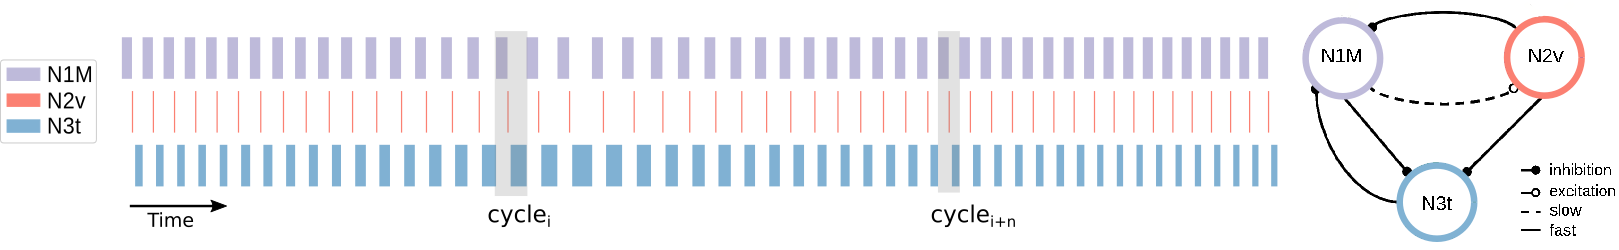
\includegraphics[width=\textwidth]{img/invariants/variability/sequences_in_cpgs.png}
	\caption{Example of robust sequential bursting dynamics in CPGs. Representation of burst duration in 3 neurons in a CPG model, the sequential activation of the three neurons conform cycles (transparent grey boxes in the sequence). The connections between the three neurons are represented in the diagram on the right side of the panel.}
	\label{fig:sequences_in_cpgs}
\end{figure}

The sequence of intervals underlying CPG rhythms present variability in the duration of each cell activation/inactivation, which has been identified in different nervous systems, e.g. see \cite{reyes_artificial_2008,Elliott1991,martinez_short-term_2019}. Consequently to the study of variability in cycle-by-cycle sequences, we have recently found sequential dynamical invariants in the form of robust linear relationships between specific sequence intervals and the period in the pyloric CPG of shore crabs (\textit{Carcinus maenas}) \parencite{elices_robust_2019}. Dynamical invariants represent constraints of particular sequence intervals in relation to different intervals in the same cycle as the instantaneous duration of the period and build rules for the overall flexibility of the rhythm. It is important to note that not all intervals composing the sequence display such constraints. The presence of invariants in the crustacean pyloric CPG are observed in all control conditions as well as in experiments under the effect of ethanol, which induces irregular rhythms \parencite{elices_robust_2019}. 

%\red{Moreover, different experimental cases are described in this study, including recordings with ethanol and PTX application. The invariants were found to be present even under those circumstances which alter the neurons activity and their variability}.

%settle an evidence in the strong relation between the sequential activation and the period duration, highlighting the importance of the temporal variability which is always present in the same intervals.

While the existence of phase maintenance and linear relationships between rhythm intervals and the period have been discussed before in convenient animal models, e.g. \cite{grillner_generation_1976,hooper_phase_1997,vavoulis_dynamic_2007}, detailed characterization of cycle-by-cycle variability to understand the existence of these relationships and the corresponding analysis of the universality of robust dynamical invariants are pending in both computational models and living recordings. The observation of this restriction in other animal models, can also support the association of these temporal restrictions to a functional, biological meaning.

During this chapter we will characterized the sequence interval variability in a model of the \textit{L. stagnalis} feeding CPG inducing variability with a ramp current injection, we will also address the issue of variability in models to study this kind of phenomena, and explore and discuss the presence of sequential dynamical invariants in living intracellular recordings as well as their possible functional role by inducing the activity from different methods but also from a practical approach in robotics. 

%In particular, a thorough analysis of interval variability in CPG models and their use in understanding the generation of dynamical invariants within specific time intervals have not been addressed. The main difficulty to study the functional balance between flexibility and robustness in sequences generated by theoretical models is the lack of variability both in the intrinsic and network dynamics. In this paper, we report the characterization of sequence interval variability in a model of the \textit{Lymnaea} feeding CPG.  By using ramp current injection protocols, it is possible to induce variability in the collective activity of the neurons of this CPG model. This enables the study of the evoked variability of the intervals conforming each cycle following the same interval definitions from \cite{elices_robust_2019}, as well as the conceivable presence of dynamical invariants, which we address here. 


\section{Methods}

\subsection{Time references, intervals and CPG sequence}
\label{subsec:intervals}
The variability study addressed in this chapter is based on the characterization of cycle-by-cycle intervals in the rhythm produced by the model CPG.
In our analysis of variability, we assess the presence of linear relationships between the intervals that build the sequence and the cycle-by-cycle period to characterize and unveil similar dynamical invariants as those found in the stomatogastric CPG \cite{elices_robust_2019}. 
The intervals here analyzed can be measured for any three neurons following a robust triphasic rhythm. In this paper N1, N2 and N3 represent the feeding CPG phases, represented in the model by interneurons N1M, N2v and N3t, respectively and in the experimental data by different combinations of moto- and interneurons.

\begin{figure}[hbt!]
	\centering
	\begin{minipage}{\textwidth}
		\centering
		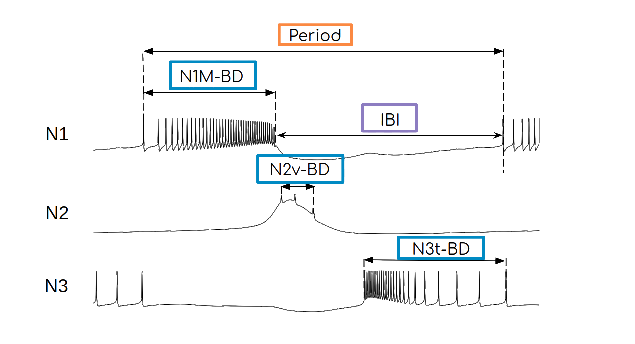
\includegraphics[width=0.8\textwidth]{img/methods-paper-modelo/figure4a.eps} 
		\label{fig:intervals_bd}
	\end{minipage}
	% \hfill
	
	\vspace{1cm}
	\begin{minipage}[t]{\textwidth}
		\centering
		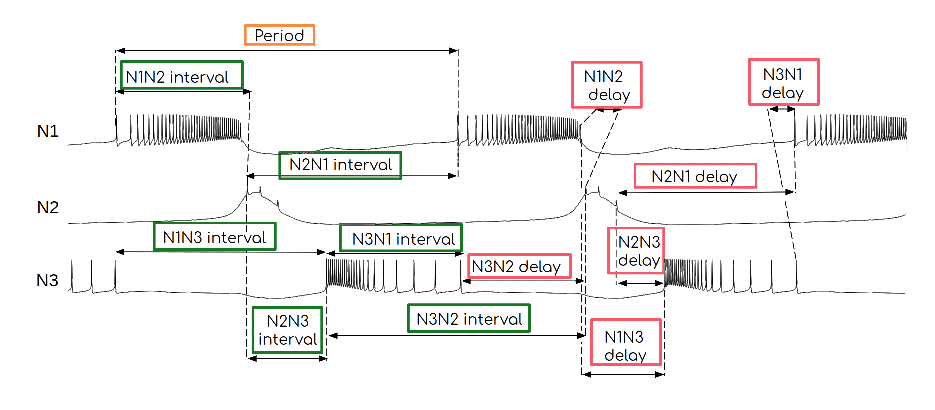
\includegraphics[width=\textwidth]{img/methods-paper-modelo/figure4b.eps} 
		\label{fig:intervals_der}
	\end{minipage}
	
	\caption{\textbf{Panel A}. Individual neuron sequence interval definitions. Each BD label represents the burst duration, defined as the time interval from the first spike to the last spike in the neuron's burst. Period was measured as the interval from the first spike of N1 burst to the first spike of the next N1 burst, covering three phases %(N1M,N2v, N3t) 
		in relation to the activity of the other neurons. IBI represents the interburst interval, defined as the time from the last spike of a neuron's burst to the first one of the next burst in the same neuron.
		\textbf{Panel B}. Definition of intervals involving pairs of neurons. NXNY interval represents interval from NX start to NY start. NXNY delay represents interval from NX end to NY start. Period was measured from N1 start to N1 start, covering the three phases of the CPG rhythm.
	}
	
	\label{fig:intervals}
\end{figure}


This is illustrated in Fig. \ref{fig:intervals}, where single neuron intervals and intervals defined between neurons are depicted and the definition of each interval is as follows:
\begin{enumerate}
	\item \textbf{Burst Duration (BD)}, measured as the time interval between the first and the last spike of the burst (start to end in the trace of a given neuron).
	\item \textbf{Inter Burst Interval (IBI)}, characterized as the difference between the last spike of a burst and the first one of the next one (end to start in the trace of a given neuron).
	\item \textbf{Period}, which envelops the bursts from the three neurons, measured as the distance between the first spike of one burst in a neuron and the first spike of the next one on that neuron (start to start).
	\item \textbf{NeuronX-NeuronY interval}, this interval is measured from the start of the burst of neuron X to the start of the burst of neuron Y (start X to start Y).
	\item \textbf{NeuronX-NeuronY delay}, being the time lapse between the burst end of a neuron X and the burst beginning of neuron Y. (end X to start Y).
\end{enumerate}

\subsection{Inducing variability in the model by current injection}
\label{subsec:inj protocol}
The spiking-bursting activity of the model CPG neurons can be modulated by using an additional current injection on each cell, implemented in the \(i_{inj}\) term of equation (\ref{eq:soma}), as performed in many experimental protocols. Depending on the current value applied, the corresponding neuron dynamics changes. While for N2v a change in this injection corresponds to a change in burst frequency (i.e. the number of bursts increases/decreases), for the rest of the neurons in the model a change in \(i_{inj}\) affects burst duration for N3t and SO, and the length of the depolarization phase in N1M.


\begin{figure}[hbt!]
	\centering
	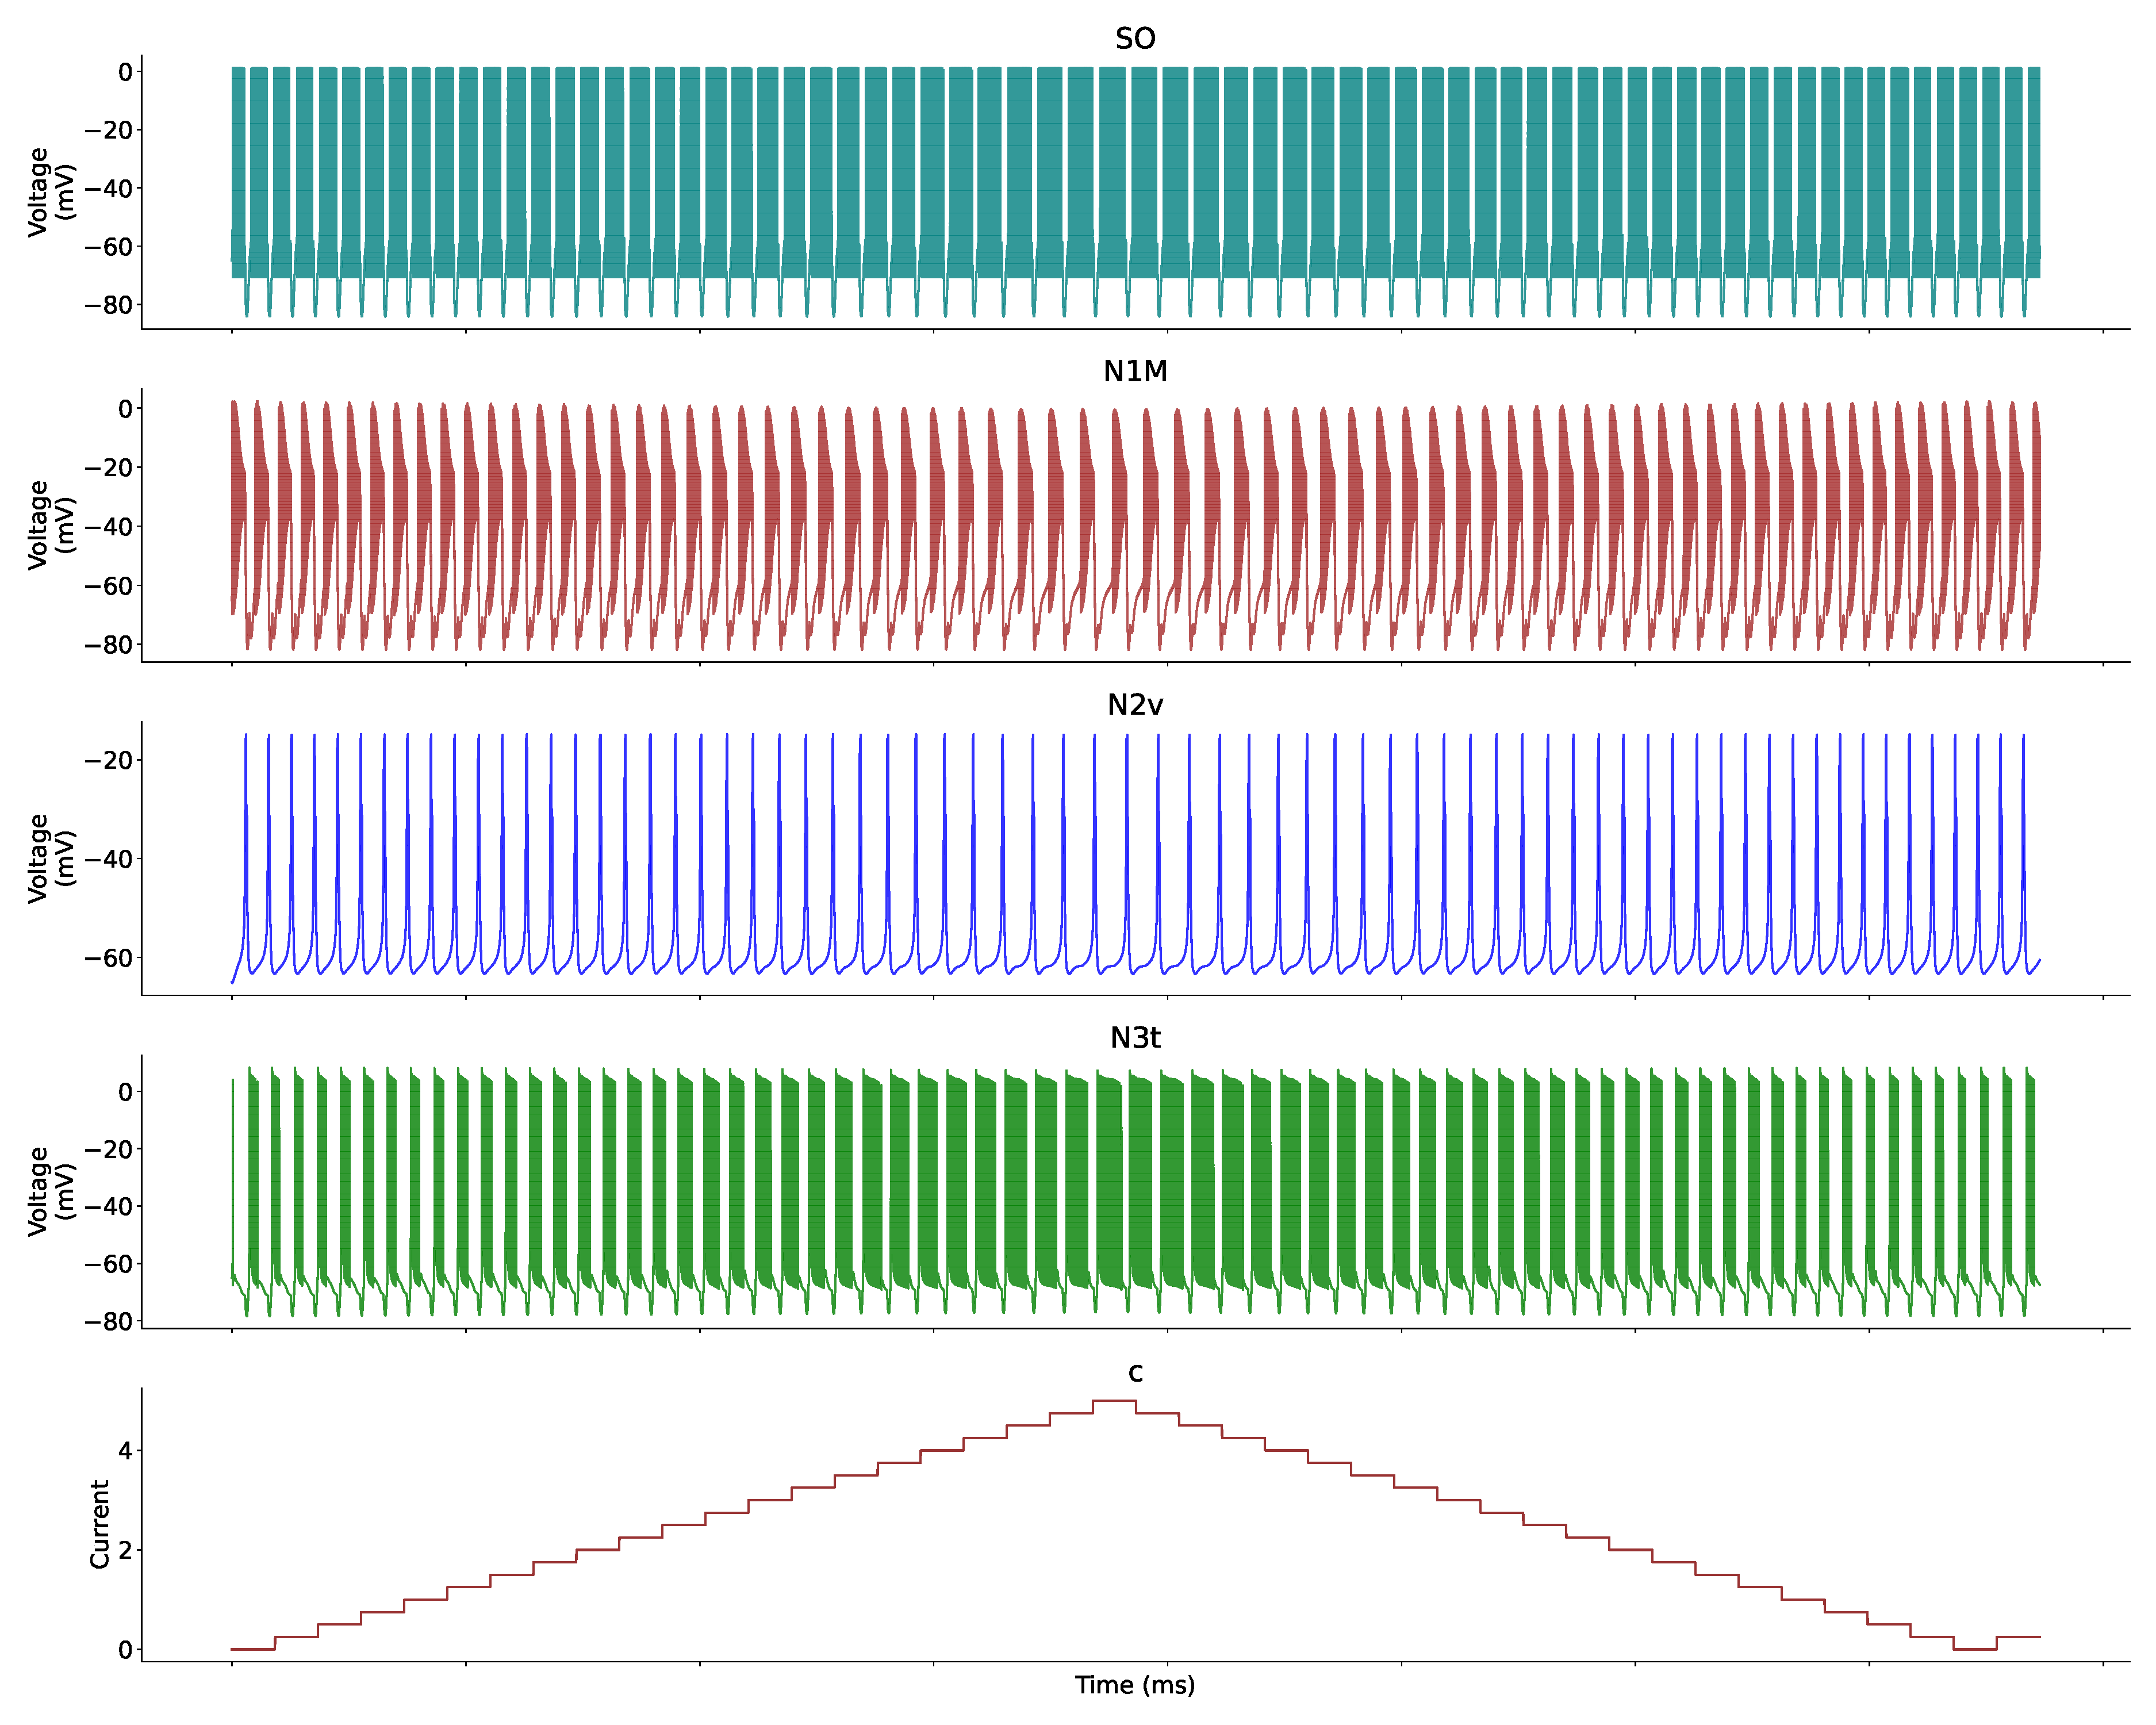
\includegraphics[width=\textwidth]{img/methods-paper-modelo/circuit_w_current.pdf}
	\caption{Illustration of the CPG activity when a current ramp \(i_{inj}\) is applied to N3t. Variability in the sequence intervals was induced by applying two consecutive ramps as the one shown in this figure into different cells.  }
	\label{fig:complete ramp example}
\end{figure}

Whilst the single neuron model descriptions have no intrinsic variability, the effect produced by the modulation of the injected current in each neuron induces variability into the circuit, which allows characterizing the sequence intervals and the period, the associated robustness of the rhythm and the presence of dynamical invariants. Such stimulation has been used previously in the living circuit, as reported by \cite{Elliott1991}. The authors of this work showed that it is possible to activate the feeding CPG with variability caused by current injection into individual cells in the circuit. CPG rhythms obtained under this type of stimulation differ depending on which neuron is being stimulated. To induce variability in the model we used a ramp protocol resulting in circuit time-interval variations as in Fig. \ref{fig:complete ramp example}.

% Even though this CPG model do not present intrinsic variability, thanks to the current \(i_{inj}\), variability is induced into the model, effectively changing burst duration. This current injection has also been used in Lymnaea preparation in living elements, stimulating N1M and SO, obtaining rhythm. Neural sequences obtained after the stimulation differ one another depending on which neuron is being stimulated. 


By varying the current injected into N1M, its burst duration is kept nearly constant, but its depolarization phase before the spiking activity begins becomes longer. Since N3t is the neuron fitting in the sequence in that phase (see Fig. \ref{fig:model simulation}), it also increases its burst duration, being the most variable one in the CPG rhythm. 

When value \(i_{inj}\) is increased on neuron SO, its burst duration becomes longer. Since SO has a modulator effect over N3t and N1M, it also alters the burst duration of these two neurons.

Neuron N3t also shows variable burst duration when an evolving current is injected. When \(i_{inj}\) value on N3t is larger, its burst duration increases, elongating the N1M depolarization phase.  

Finally, when current is applied to N2v the effect on its burst duration or the burst duration of the rest of the neurons is rather small. However, \(i_{inj}\) % current 
modulates N2v burst frequency through the hyperpolarization phase. 

%cambios
Therefore, we used a current ramp protocol to induce variability in the CPG model defined as follows: a ramp variable $c$, which controlled the current injection value ($i_{inj}=c$) on the neuron being stimulated, was increased from a minimum to a maximum value, and then decreased back to the initial value. This was repeated twice in each simulation. The ramp variable was modified with a fixed step value every 4.6 seconds (the approximate duration of two N3t bursts). The minimum and maximum $c$ values were different in each cell and were tuned to generate realistic spiking-bursting behavior. All parameters used for the simulation analyses reported in this paper are summarized in Table \ref{table:inj values}.

\begin{table}[h!]
\centering
\begin{tabular}{c|cccc|c|ccc|}
\multirow{2}{*}{\textbf{\begin{tabular}[c]{@{}c@{}}Neuron\\ stimulated\end{tabular}}} & \multicolumn{4}{c|}{\textbf{\(i_{inj}\) value}}                 & \multirow{6}{*}{} & \multicolumn{3}{c|}{\textbf{Ramp values ($c$)}}   \\ \cline{2-5} \cline{7-9} 
                                                                                      & \textbf{SO} & \textbf{N1M} & \textbf{N2v} & \textbf{N3t} &                   & \textbf{Min} & \textbf{Max} & \textbf{Step} \\ \cline{1-5} \cline{7-9} 
\textbf{N1M}                                                                          & 8.5         & $c$            & 2            & 0            &                   & 0            & 10.5         & 0.5           \\ \cline{1-5} \cline{7-9} 
\textbf{N3t}                                                                          & 9           & 10           & 1            & $c$            &                   & 0            & 5            & 0.25          \\ \cline{1-5} \cline{7-9} 
\textbf{SO}                                                                           & $c$           & 10           & 1            & 4            &                   & 8.2          & 13           & 0.25          \\ \cline{1-5} \cline{7-9} 
\end{tabular}
\caption{List of \(i_{inj}\) values that yield realistic bursting rhythms for each neuron in the model CPG used in the stimulation protocols reported in this paper. The left section of the table displays the \(i_{inj}\) values applied to each neuron (columns) during each simulation condition (rows). Ramp values on the right section refer to the minimum and maximum values of the ramp variable $c$ in each simulation, increasing \(i_{inj}\) in the specified step every 4.6 seconds (the approximate duration of two N3t burst) to induce variability.} \label{table:inj values}
\end{table}

Simulations of \cite{vavoulis_computational_2007} model were implemented in C++. The code of the feeding CPG model implementation is available at \href{github.com/GNB-UAM/CPG-feeding-Lymnaea}{https://github.com/GNB-UAM/CPG-feeding-Lymnaea}. This model was also included in Neun library in a Github repository \href{github.com/GNB-UAM/Neun}{https://github.com/GNB-UAM/Neun}. Each simulation had the duration of two consecutive cycles of up and down ramps as the one shown in Fig. \ref{fig:complete ramp example} using the parameters described in Table \ref{table:inj values}. The number of bursts in each simulation was approximately 140 (this number slightly depends on the neuron stimulated). Parameter values such as reversal potentials and synaptic conductances were the same ones specified in \cite{Vavoulis2007}.


% \subsection{Model simulation specifications and statistical analysis}\todo{añadir en métodos generales o ampliarlo también a experimental}



\subsection{Experimental recordings and stimulation}
The experimental recordings analyzed in section \ref{sec:experimental sussex} were performed by Michael Crossley, University of Sussex, and kindly provided for this work. 

Each recording had at least 5 microelectrodes, which allowed to characterize the rhythm based on combinations of different neuron's activity. There are cases of experiments in that section:
\begin{itemize}
	\item Spontaneous activity: After the isolation of the CNS, the electrodes impailed in the neuron recorded the spontaneous activity in the CPG, with no further stimulation.
	\item Nerve electrical stimulation: For the activation of the rhythm it is possible to stimulate the median lip nerve (MLN). The data analyzed there was stimulated by a 4V stimulous at 1Hz. 
	\item Neuron electrical stimulation: To modulate the CPG rhythm, SO and CV1a neurons where stimulated (in different experiments) by injecting a constant depolarizing current.
\end{itemize}

%To define each phase, we used different neurons and bursting references, depending on the ones available on the circuit, following intervals definition in table \ref{table:cpg ref intervals}.
%
%For each recording each phase was defined as follows:
%
%\paragraph{Spontaneous Activity Example 1}
%N1 phase was analyzed from B1 activity (bursting and depolarization); N2 phase was analyzed from B5 hyperpolarization, which has a strong inhibition from N2v; N3 phase was analyzed from the bursting activity of B8, that replicates the N3t duration. 
%
%\paragraph{Spontaneous Activity Example 2}
%N1 phase was analyzed from B1 activity (bursting and depolarization); N2 phase was analyzed from B1 hyperpolarization, which has a strong inhibition from N2v; N3 phase was analyzed from the bursting activity of B8, that replicates the N3t duration. 
%Since the reference for N2 here coincides with N1 reference, we display here only the intervals corresponding to N1 and N3 phases, since the intervals that correspond to 3 phases, such as N1-N2 delay or N2-N3 delay, either are already represented in the defined intervals or have a duration close to 0 ms.
%
%\paragraph{Spontaneous Activity Example 3}
%N1 phase was analyzed from B1 activity (bursting and depolarization); N2 phase was analyzed from B5 hyperpolarization, which has a strong inhibition from N2v; N3 phase was analyzed from the bursting activity of B8, that replicates the N3t duration. 
%
%\paragraph{Spontaneous Activity SO modulation}
%N1 phase was analyzed from B1 activity (bursting and depolarization); N2 phase was analyzed from B5 hyperpolarization, which has a strong inhibition from N2v; N3 phase was analyzed from the bursting activity of B8, that replicates the N3t duration. 




\subsection{Models with chaotic activity}

\subsubsection{LP model by \cite{nowotny_probing_2008}}

The membrane potential of axon and soma compartment, $V_{\text{axon}}$ and $V_{\text{soma}}$ respectively, are described by

\begin{equation}
	\frac{dV_{\text{axon}}}{dt} = \frac{1}{C_a} \left( -I_{\text{Na}} - I_{\text{Kd}} - I_M - I_{\text{leak,a}} + I_{VV} \right)
\end{equation}

\begin{equation}
	\frac{dV_{\text{soma}}}{dt} = \frac{1}{C_s} \left( -I_{\text{Ca}} - I_{\text{KCa}} - I_A - I_h - I_{\text{leak,s}} - I_{VV} + I_{\text{scale}} (I_{\text{DC}} - I_{\text{offset}} + I_{\text{syn}} \right))
\end{equation}

$I_{\text{offset}} = 2 \, \text{nA}$ stems from the residual coupling at the end of the parameter estimation procedure which introduces a current bias due to differences in baseline voltage of data and model (on top of $V_{\text{shift}}$). $I_{\text{syn}}$ denotes the total incoming synaptic current. All ionic currents except for the ones mentioned explicitly below are given by

\begin{equation}
	I_x = g_x m^p h^q (V - V_x)
\end{equation}

where $g_x$ is the maximal conductance of the current, $V$ is the membrane potential of either the axon compartment ($I_{\text{Na}}$, $I_{\text{Kd}}$, and $I_M$) or the soma compartment (all other currents), and $V_x$ is the reversal potential of the current. The activation and inactivation variables are governed by

%\begin{equation}
%	\frac{dm}{dt} = \alpha_m (1 - m) - \beta_m m
%\end{equation}
%
%\begin{equation}
%	\frac{dh}{dt} = \alpha_h (1 - h) - \beta_h h
%\end{equation}
%
%for $I_{\text{Na}}$ and $I_{\text{Kd}}$, and
%
%\begin{equation}
%	\frac{dm_x}{dt} = \frac{m_{\infty,x}(V) - m_x}{\tau_{m_x}}
%\end{equation}

\subsubsection{Non chaotic model \cite{ghigliazza_minimal_2004}}
\todo{revisar}
The Ghigliazza and Holmes model for motoneurons is described by the following equations:

1. The membrane potential dynamics of a neuron is given by:

\begin{equation}
	C_m \frac{dV}{dt} = -\sum I_x + I_{\text{syn}}
\end{equation}

where \( C_m \) is the membrane capacitance, \( V \) is the membrane potential, \( I_x \) are the various ionic currents, and \( I_{\text{syn}} \) is the synaptic current.

2. The ionic currents \( I_x \) are typically given by:

\begin{equation}
	I_x = g_x m^p h^q (V - V_x)
\end{equation}

where \( g_x \) is the maximal conductance, \( m \) and \( h \) are the activation and inactivation variables, \( p \) and \( q \) are the respective powers, and \( V_x \) is the reversal potential of the current.

3. The gating variables \( m \) and \( h \) are governed by first-order kinetics:

\begin{equation}
	\frac{dm}{dt} = \alpha_m (1 - m) - \beta_m m
\end{equation}

\begin{equation}
	\frac{dh}{dt} = \alpha_h (1 - h) - \beta_h h
\end{equation}

where \( \alpha_m \), \( \beta_m \), \( \alpha_h \), and \( \beta_h \) are voltage-dependent rate constants.

4. For a central pattern generator (CPG), the model includes a set of coupled differential equations to describe the rhythmic activity:

\begin{equation}
	\frac{d\phi_i}{dt} = \omega_i + \sum_j K_{ij} \sin(\phi_j - \phi_i - \psi_{ij})
\end{equation}

where \( \phi_i \) is the phase of the \( i \)-th oscillator, \( \omega_i \) is the intrinsic frequency, \( K_{ij} \) is the coupling strength between oscillators \( i \) and \( j \), and \( \psi_{ij} \) is the phase shift.



\subsection{Hybrot structure}

We have designed and implemented a FLC-Hybrot, a hybrot controlled by the neural activity of a living and functional pyloric CPG, to validate the importance of the balance between robustness and flexibility in this circuit, as provided by cycle-by-cycle dynamical invariants present in its dynamics \cite{Elices2019}. With this idea in mind we built an hexapod robot whose legs performed oscillatory motions to move forward. The period and amplitude of these oscillations were determined by the sequential cycle-by-cycle activity of the CPG neurons. At the same time, the hybrot included a light sensor and sent feedback information regarding the light conditions around it back to the neural circuit in the form of an electrical current. These stimuli modified the behaviour of the cells, resulting in a change of the hybrot locomotion, preserving always the required motor coordination, and therefore forming a real-time closed-loop interaction among living and electronic components (Figure \ref{fig:robot_results_summary}). The goal of the FLC-Hybrot is to demonstrate that a dynamical principle of the functional living circuit can be used to coordinate the locomotion with sensory feedback from the robot. In our case, we use the presence of dynamical invariants in the form of robust relationships between the time intervals that build the cycle-by-cycle activity of the CPG, which are sustained under any circumstance even when there are external inputs to the circuit, to modulate the behavior of the robot. \todo{copia pega de paper robot adaptar}

\begin{figure}[h!]
	\begin{center}
		% \includegraphics[width=\linewidth]{images/robot/robot_results_summary}
		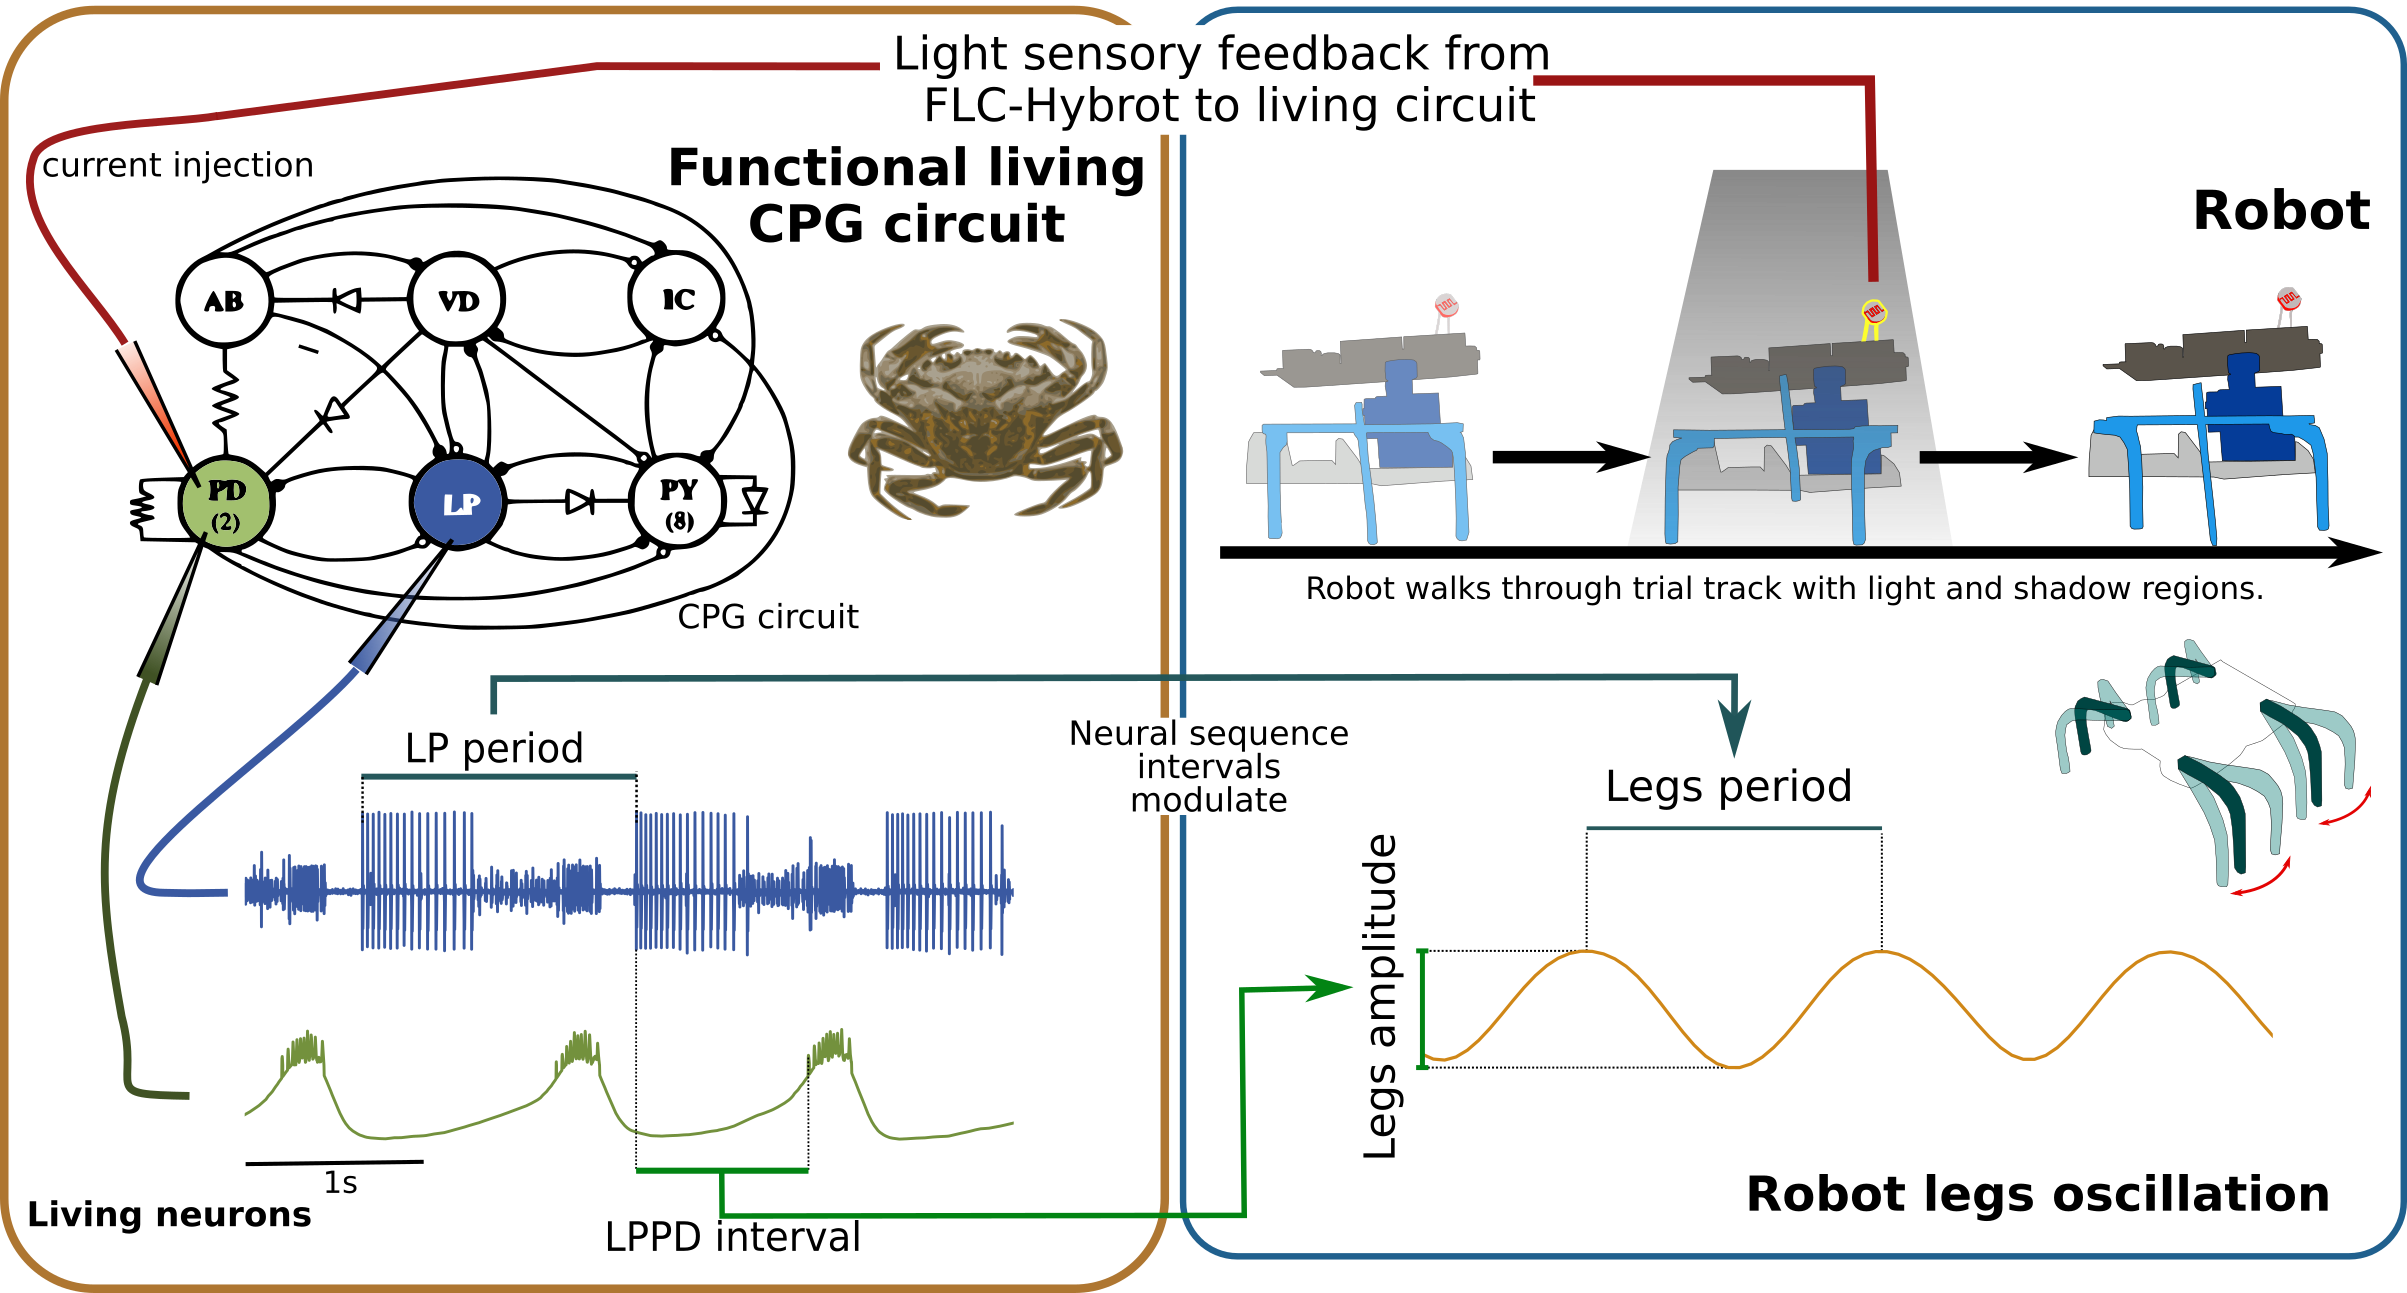
\includegraphics[width=\linewidth]{img/invariants/robot/Figure1_experiment_design_v1.png}
	\end{center}
	\caption{Representation of the FLC-Hybrot paradigm design. Neural dynamics from a functional living CPG circuit are recorded online and used to coordinate the robot movement in real-time. Activity from the PD neuron is recorded intracellularly (green trace), while the LP bursts are extracted from the nerve's extracellular signal (blue trace). This robot walks through a trial track with interspersed light and shadow regions. When the robot's light sensor detects that it is located under a shadow, it sends feedback current to the living circuit. CPG dynamics change as a reaction to the injected current, thus modifying the robotic locomotion. The following video shows an example of this experiment \url{https://youtu.be/ny2dJGbG8lo}.}
	\label{fig:robot_results_summary}
\end{figure}





\section{Sequential dynamical invariants in computational models}
\label{c-invariants-model}
In this section we will investigate the cycle-by-cycle sequential restrictions found in \cite{elices_robust_2019} in a computational model, the detailed reproduction of the activity allows to study in detail the mechanisms associated to the circuit and the time-interals relations. We used the feeding CPG model description of \cite{vavoulis_dynamic_2007}, which even though it does not have a chaotic mode, the model is flexible enough to adapt the variability of one of the neurons. Following the current injection protocol defined in section \ref{subsec:inj protocol}, N1M, N3t and SO neurons in the model were stimulated for our analysis of the sequence interval variability. Using this induced variability we were able to explore the presence of sequential dynamical invariants under different scenarios. The effect on injecting a current ramp on N2v is not reported here since it leads to lower variability than the other cases. In all simulations, we could test the robustness of the rhythm while inducing the external perturbation that evoked variability in the search for dynamical invariants. The results summarized and adapted for this section were published in \cite{garrido-pena_characterization_2021}.

First we saw in the simulations is that the model of the feeding CPG faithfully reproduces the activity of the main neurons involved in the generation of its triphasic rhythm \parencite{Vavoulis2007}. This includes their waveforms and the relationships between the cycle period and the duration of several intervals reported in \parencite{Elliott1991}. Note that, since there was not a description of a chaotic mode, all the rhythms explored here were analyzed from induced stimulation, not by simulating spontaneous activity. This was a restriction when exploring spontaneous activity, since the circuit needed to be altered by one of the neurons, simulating a extended experimental protocol, but still altering the circuit in a predefined way. Also, other phenomena reported in the pyloric CPG experimental work, were there was a "reset" in the inter-cycle dynamics of the dynamical invariants, could not be explored in this model, since the ramp value was progressive (see Apendix Fig. \ref{fig:N1M stimulation pairplot reset} for a representation of this non-reset output). All this will be illustrated in the following Section \ref{sec:experimental sussex} with experimental recordings and other options to reproduce the functional variability will be discussed in Sec. \ref{sec:model variability}

\subsection{N1M driven variability}
\label{subsec:n1m driven}

N1M neuron is frequently stimulated using ramp protocols in living preparations \parencite{Elliott1991} as it plays an important role in initiating the CPG rhythm. In our case, after applying the current injection protocol into N1M and detecting the spike and burst events for each neuron in the CPG model, all  intervals represented in Fig. \ref{fig:intervals} were quantified. We show in Fig. \ref{fig:invariant n1m} the variability and the correlation between the period and each interval.

\begin{figure}[hbt!]
	\begin{minipage}[b]{0.45\textwidth}
		\centering
		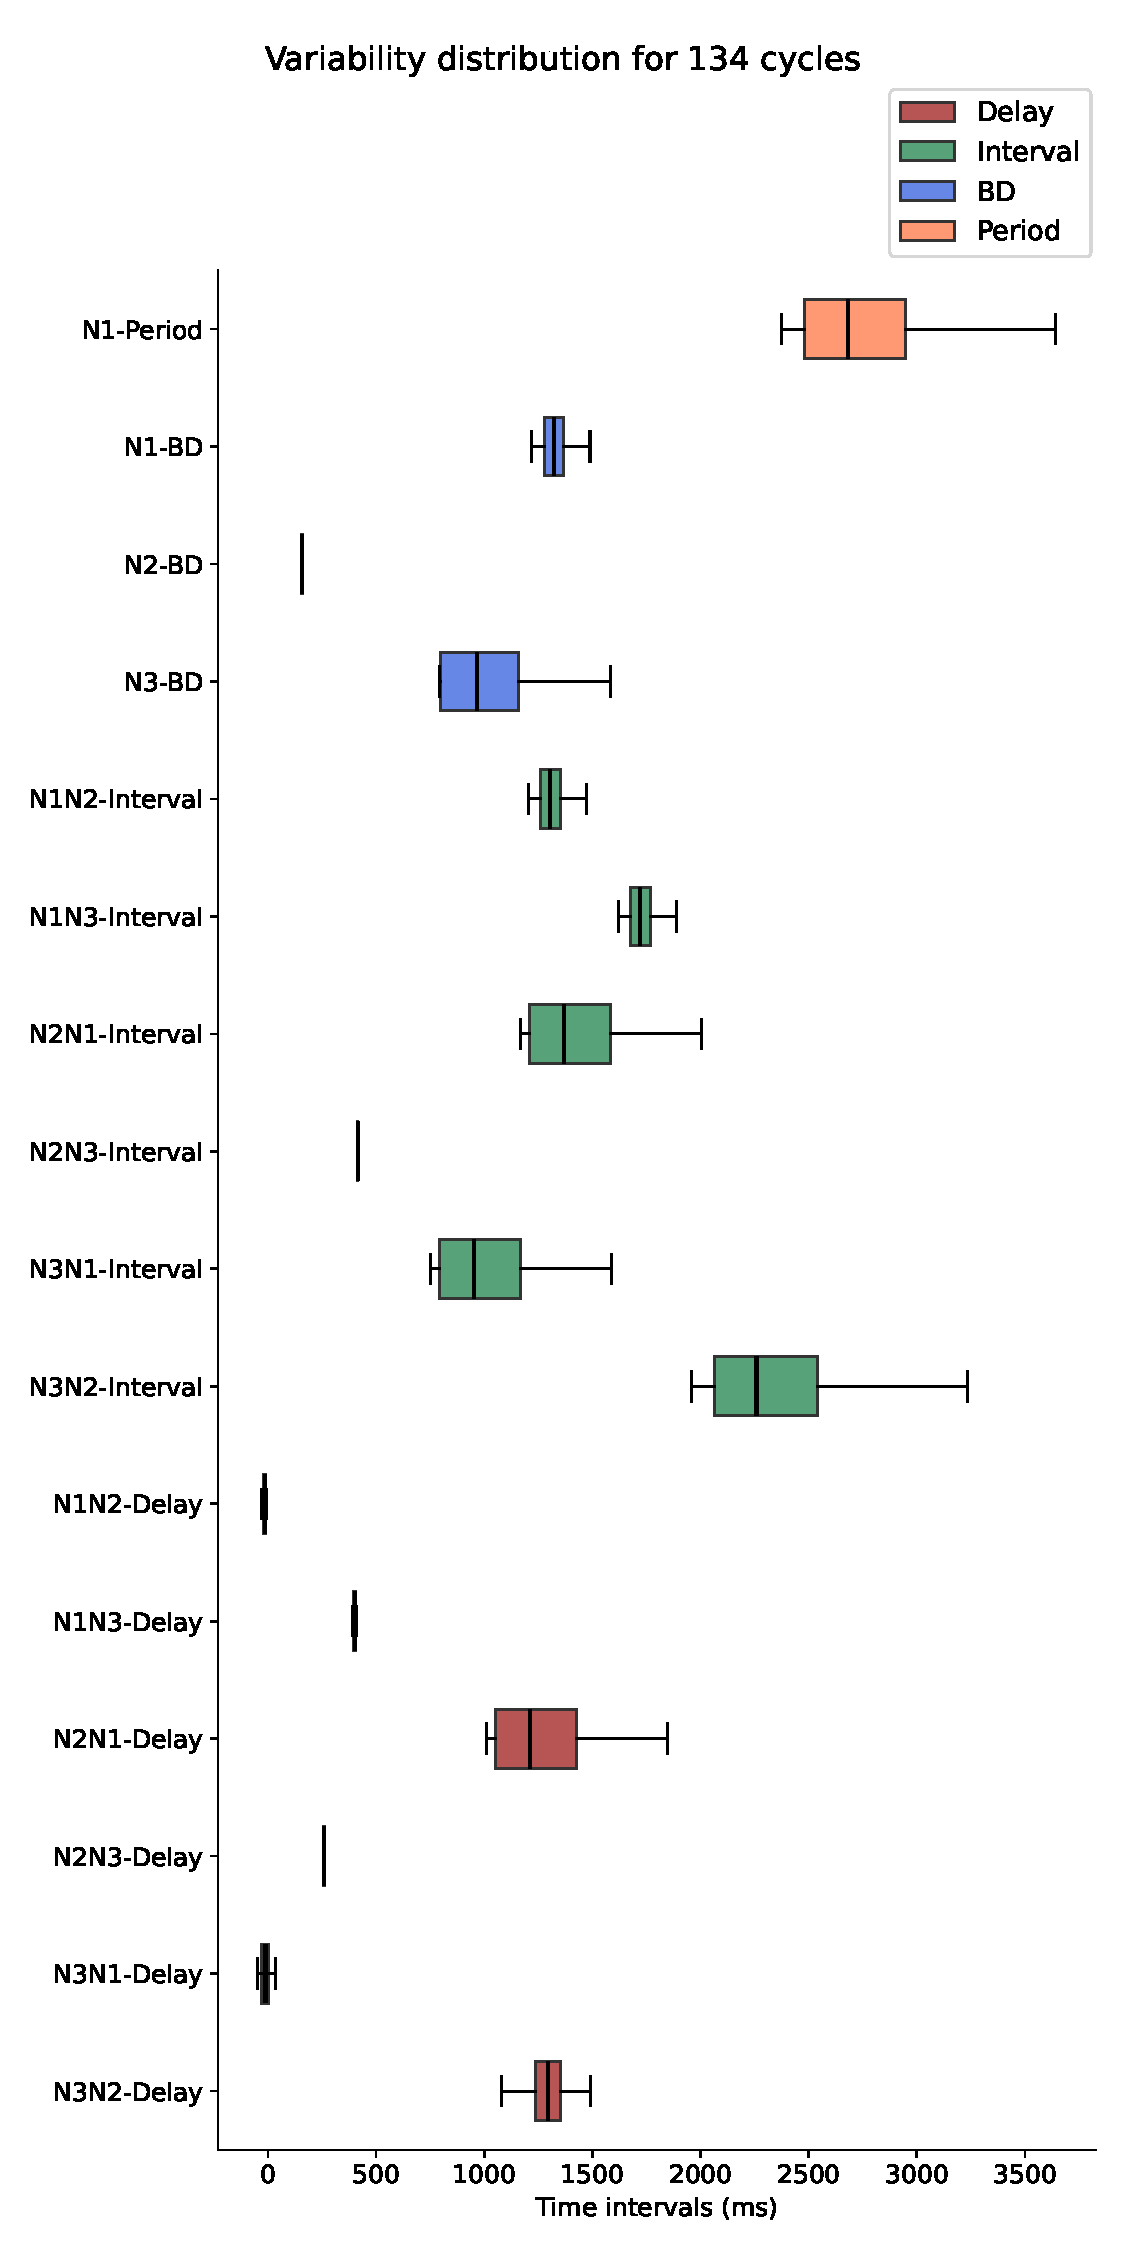
\includegraphics[width=\textwidth]{invariants/data/MODEL/n1m_driven/images/3phases/_boxplot.pdf}
	\end{minipage}
	\begin{minipage}[b]{0.53\textwidth}
		\centering
		\begin{minipage}[b]{\textwidth}
			\centering
			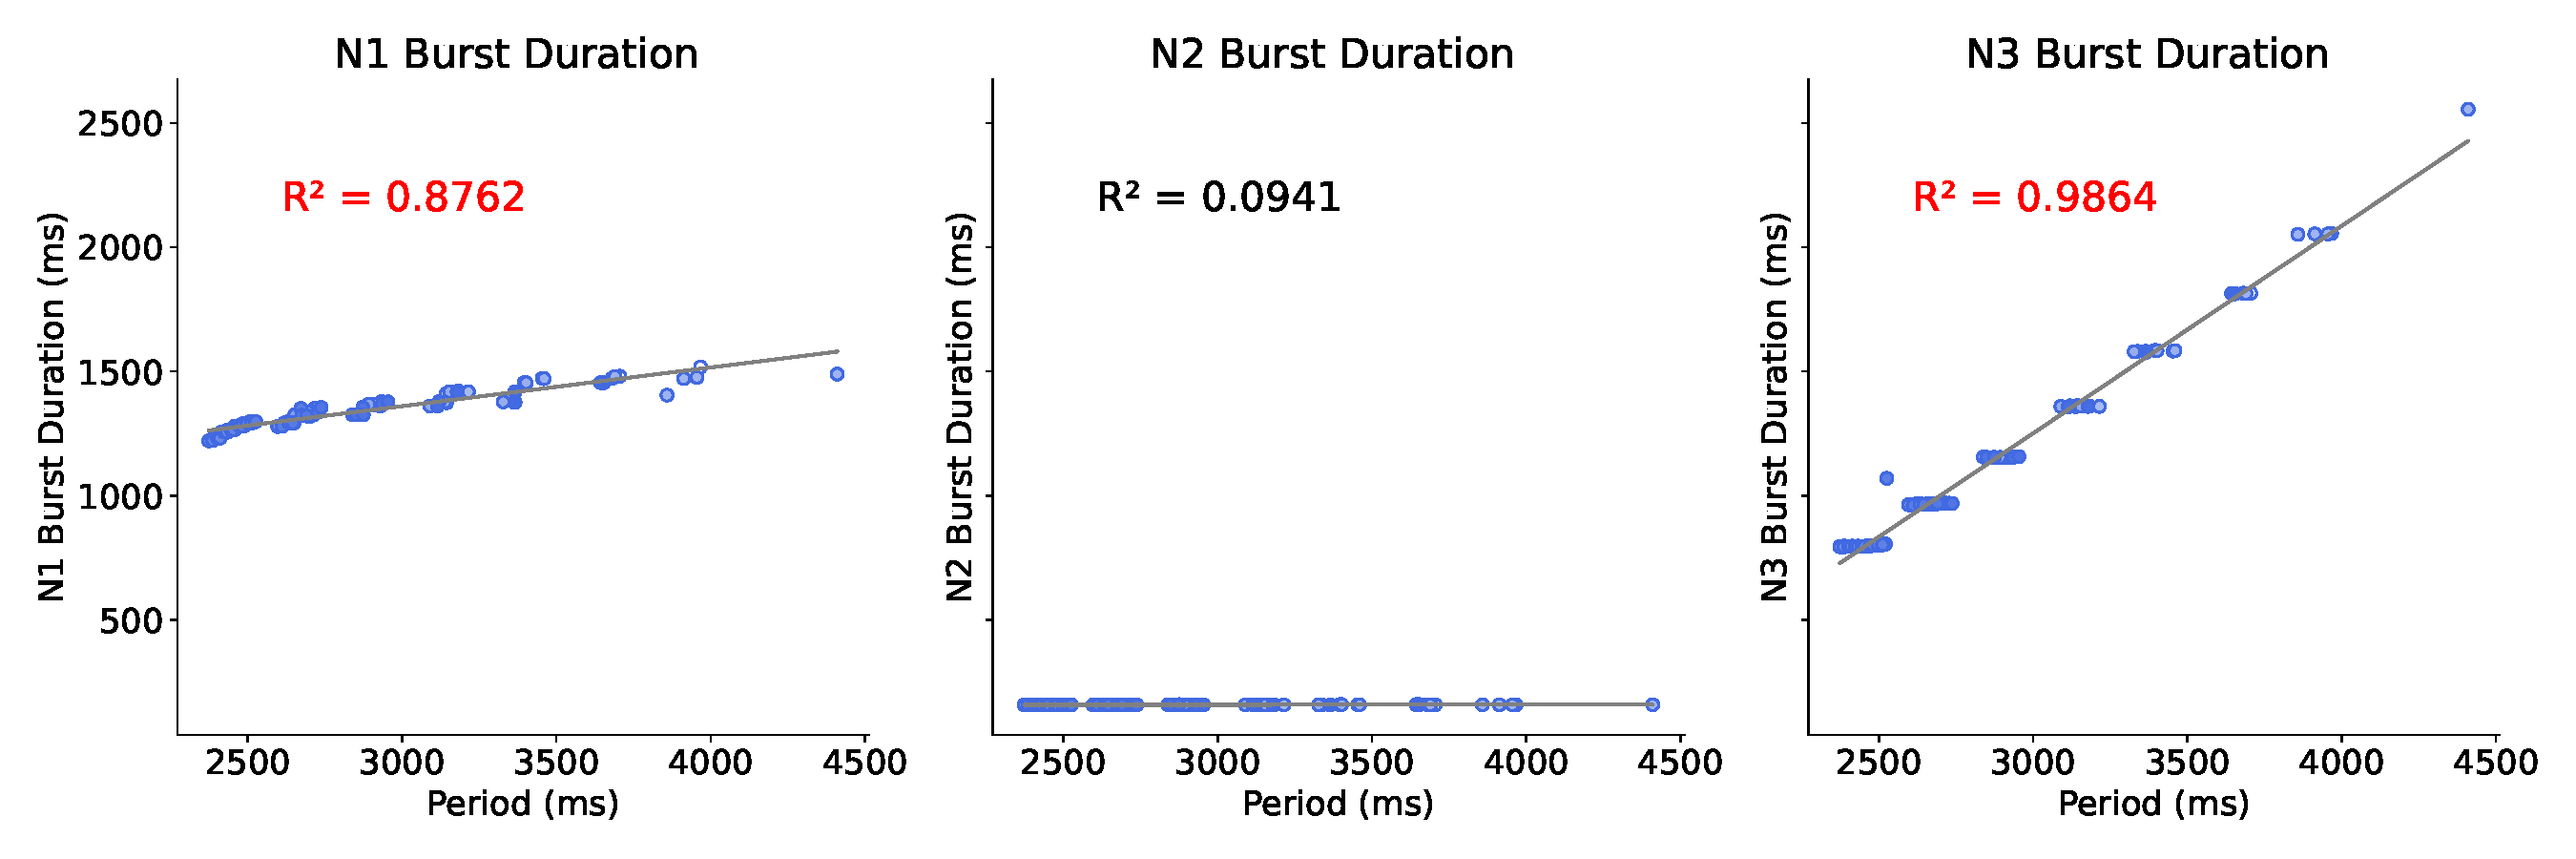
\includegraphics[width=\textwidth]{invariants/data/MODEL/n1m_driven/images/3phases/_durations.pdf}
		\end{minipage}\
		\begin{minipage}[b]{\textwidth}
			\centering
			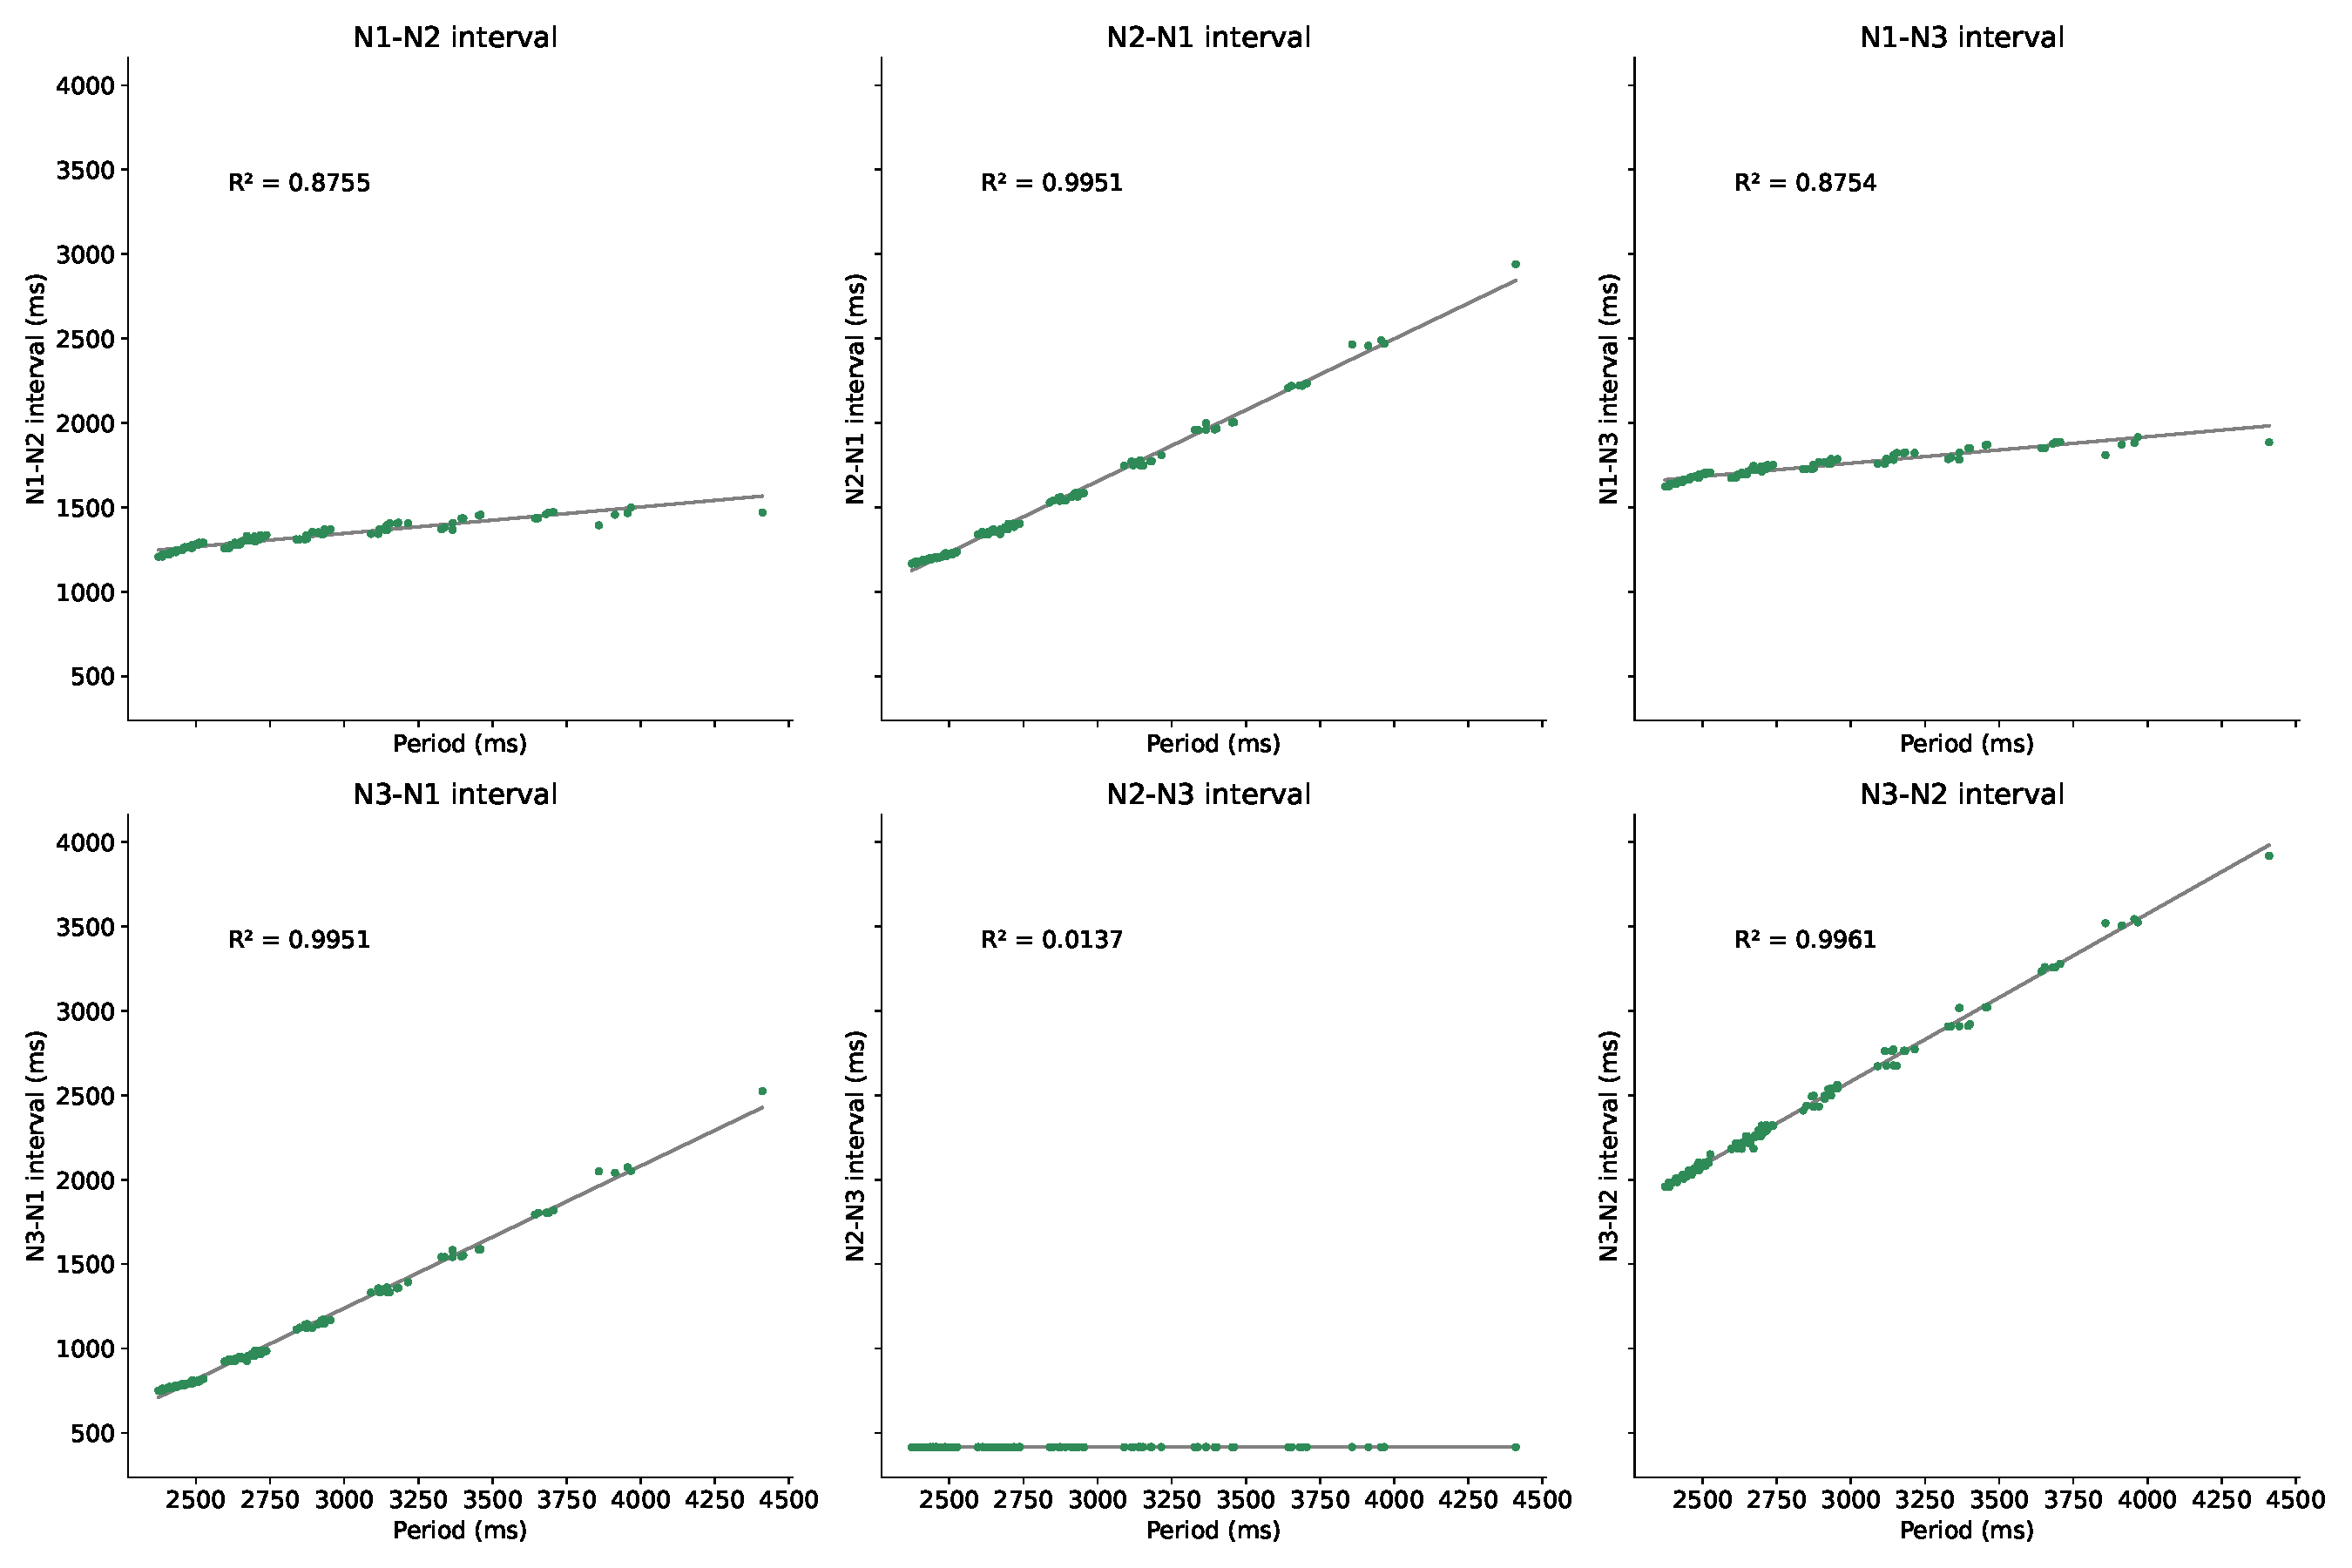
\includegraphics[width=\textwidth]{invariants/data/MODEL/n1m_driven/images/3phases/_intervals.pdf}
		\end{minipage}\
		\begin{minipage}[b]{\textwidth}
			\centering
			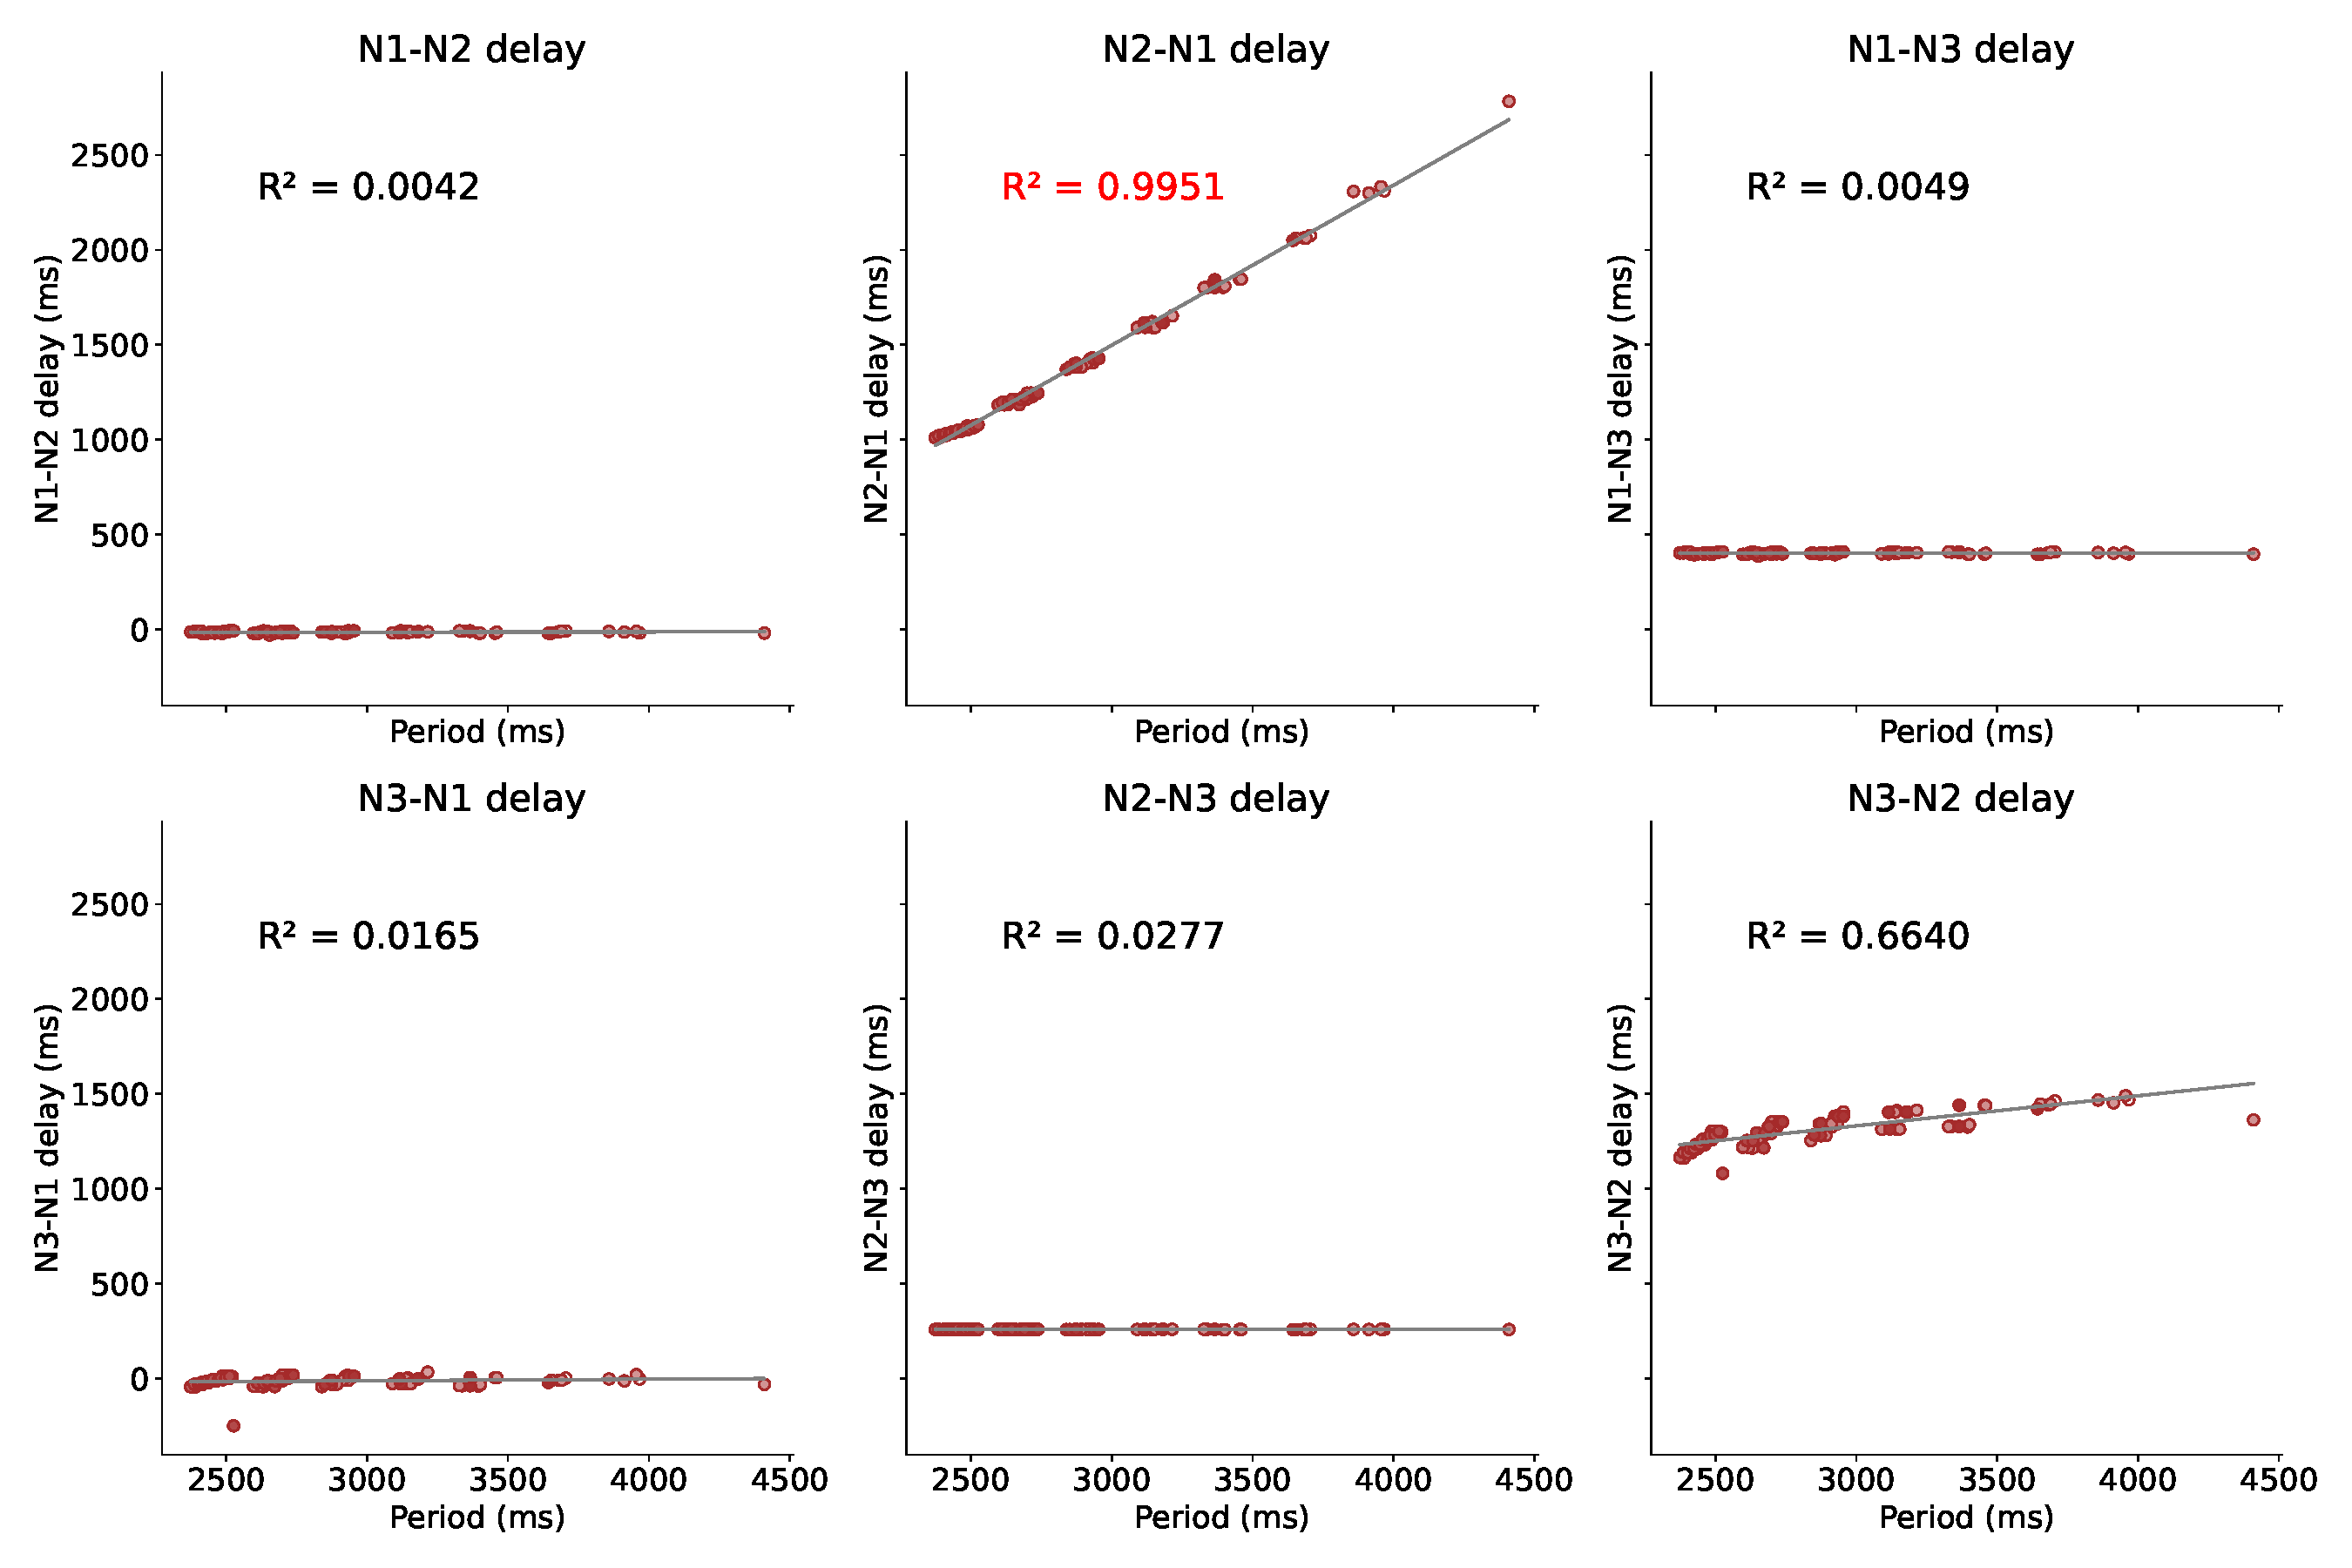
\includegraphics[width=\textwidth]{invariants/data/MODEL/n1m_driven/images/3phases/_delays.pdf}
		\end{minipage}
	\end{minipage}
	\caption{\textbf{N1M stimulation:} a) Box-plots of the  sequence intervals under N1M neuron stimulation. b) Interval correlations to period for N1M-driven simulation. First row: Burst duration. Second and third row: Two-neuron intervals. Forth and fifth row: Two-neuron delays. Linear relationships are quantified by the $R^2$ values of the linear regression.}
	\label{fig:invariant n1m}
\end{figure}

Figure \ref{fig:invariant n1m}.a) displays the boxplots of the duration of all sequence intervals defined above. Regarding burst duration of the neurons (N1M-BD, N2v-BD, N3t-BD), we can observe in this figure that the most variable one corresponds to N3t neuron. Furthermore, the derived intervals which cover N3 burst duration are also the ones presenting larger variability (i.e., N2-N1, N3-N1 and N3-N2 intervals and N2-N1 delay). On the other hand, the least variable intervals correspond to the ones related to N2v and N1M burst duration, i.e., N1-N2, N1-N3, N2-N3 intervals and N1-N2, N1-N3, N3-N1, N2-N3, N3-N2 delays. They show a nearly a constant duration during each period.

Figure \ref{fig:invariant n1m}.b) plots the cycle-by-cycle measurements of the intervals defined in \ref{fig:intervals} against the period. The first row displays burst duration intervals, which are the intervals analyzed in Elliot et al. \parencite{Elliott1991} from data obtained in electrophysiological recordings of living neurons, and in Vavoulis et al. from data obtained in model simulations \parencite{vavoulis_computational_2007}. The results shown in this row match those results, being N3t-BD the most correlated to the period, which can be noted by the $R^2$ value close to one in the linear regression. The other two intervals (N1M-BD and N2v-BD), which were also the least variable, are not strongly correlated to the period. 

Likewise, the most variable intervals derived from other time references of the sequence also show a high correlation with the period, i.e., they present dynamical invariants, in this case N2-N1, N3-N1, N3-N2 intervals and N2-N1 delay. The cycle-by-cycle period variability is a consequence of the variability in these specific intervals.

On the other hand, intervals related to neuron N2v and N1M are the least variable. N2v is the one least affected by the global activity of the circuit, in terms of its burst duration. Moreover, some of the intervals are very short, or even negative, since the end of a given neuron's burst overlaps the next one's beginning (N1-N2 and N3-N1 delay). This is the case for N1-N2 and N3-N1 delay (4th row, 1st column and 5th row, 1st column, respectively in Fig. \ref{fig:invariant n1m}.b).  




\subsection{N3t driven variability}
\label{subsec:n3t driven}

The stimulation protocol was also applied to N3t neuron. In spite that no previous analysis on injecting a current ramp into this neuron has been reported neither experimentally nor in the feeding CPG computational model, due to the connectivity in the circuit, it can be expected that stimulation of N3t will induce variability in the rhythm. The characterization of the sequence intervals in this case are shown in Fig. 
\ref{fig:invariants n3t}.a) and the correlation analysis is displayed in Fig. \ref{fig:invariants n3t}.b).
%In fact, we can expect a similar result to N1M-driven simulation because of their bidirectional connectivity see Fig. \ref{fig:CPG diagram}.  ***dicutir si es siméterica o no *****


Results shown in Fig. \ref{fig:invariants n3t}.a) indicate that the larger variability is present in the same intervals related to N3t burst duration, as when the stimulation was delivered to N1M. However, in this simulation we observe that N1M had a lower variability while N3t had a higher variability with respect to the previous condition. 
%: N1M decreased its variability while N3t has increased it *****discutir***. 
In contrast, N2v-BD maintained its variability, as well as all the derived intervals containing this burst duration.

Note that N3-N1 delay, which is the interval from the end of the N3t burst to the beginning of N1M burst, shows negative values. This means that neuron N1M started earlier than the end of N3t in every cycle. Whilst this was also present in N1M-driven activity, here the variability of this interval is much higher, leading to a larger overlapping.
% N2v maintains its variability, being this interval and all the intervals related to it the least variable. Hence, in the distribution of the activity in the circuits between the neurons, the main negotiation is between N1M and N3t, distributing the variability and the period leading between they both. ***esto también lo tenemos que pulir un poco****

Figure \ref{fig:invariants n3t}.b) plots each interval duration against the period. As in the previous condition, the dynamical invariants (i.e. intervals presenting a strong correlation to the period) show up in the intervals related to N3t, which were the ones presenting also the highest variability, whereas those intervals that do not participate in dynamical invariants, are the ones related to N1M and mostly N2v (the least variable ones). 


%The linear relationships regarding the least variable intervals (related to N2v and N1M burst durations), also present similar results to those discussed above when the rhythm was driven by N1M. Hence, the intervals most correlated are the ones with higher variability, whereas those intervals that do not participate in dynamical invariants, are the ones related to N1M and mostly N2v (the least variable ones).
%***revisar redundancia***


\begin{figure}[hbt!]
	\begin{minipage}[b]{0.45\textwidth}
		\centering
		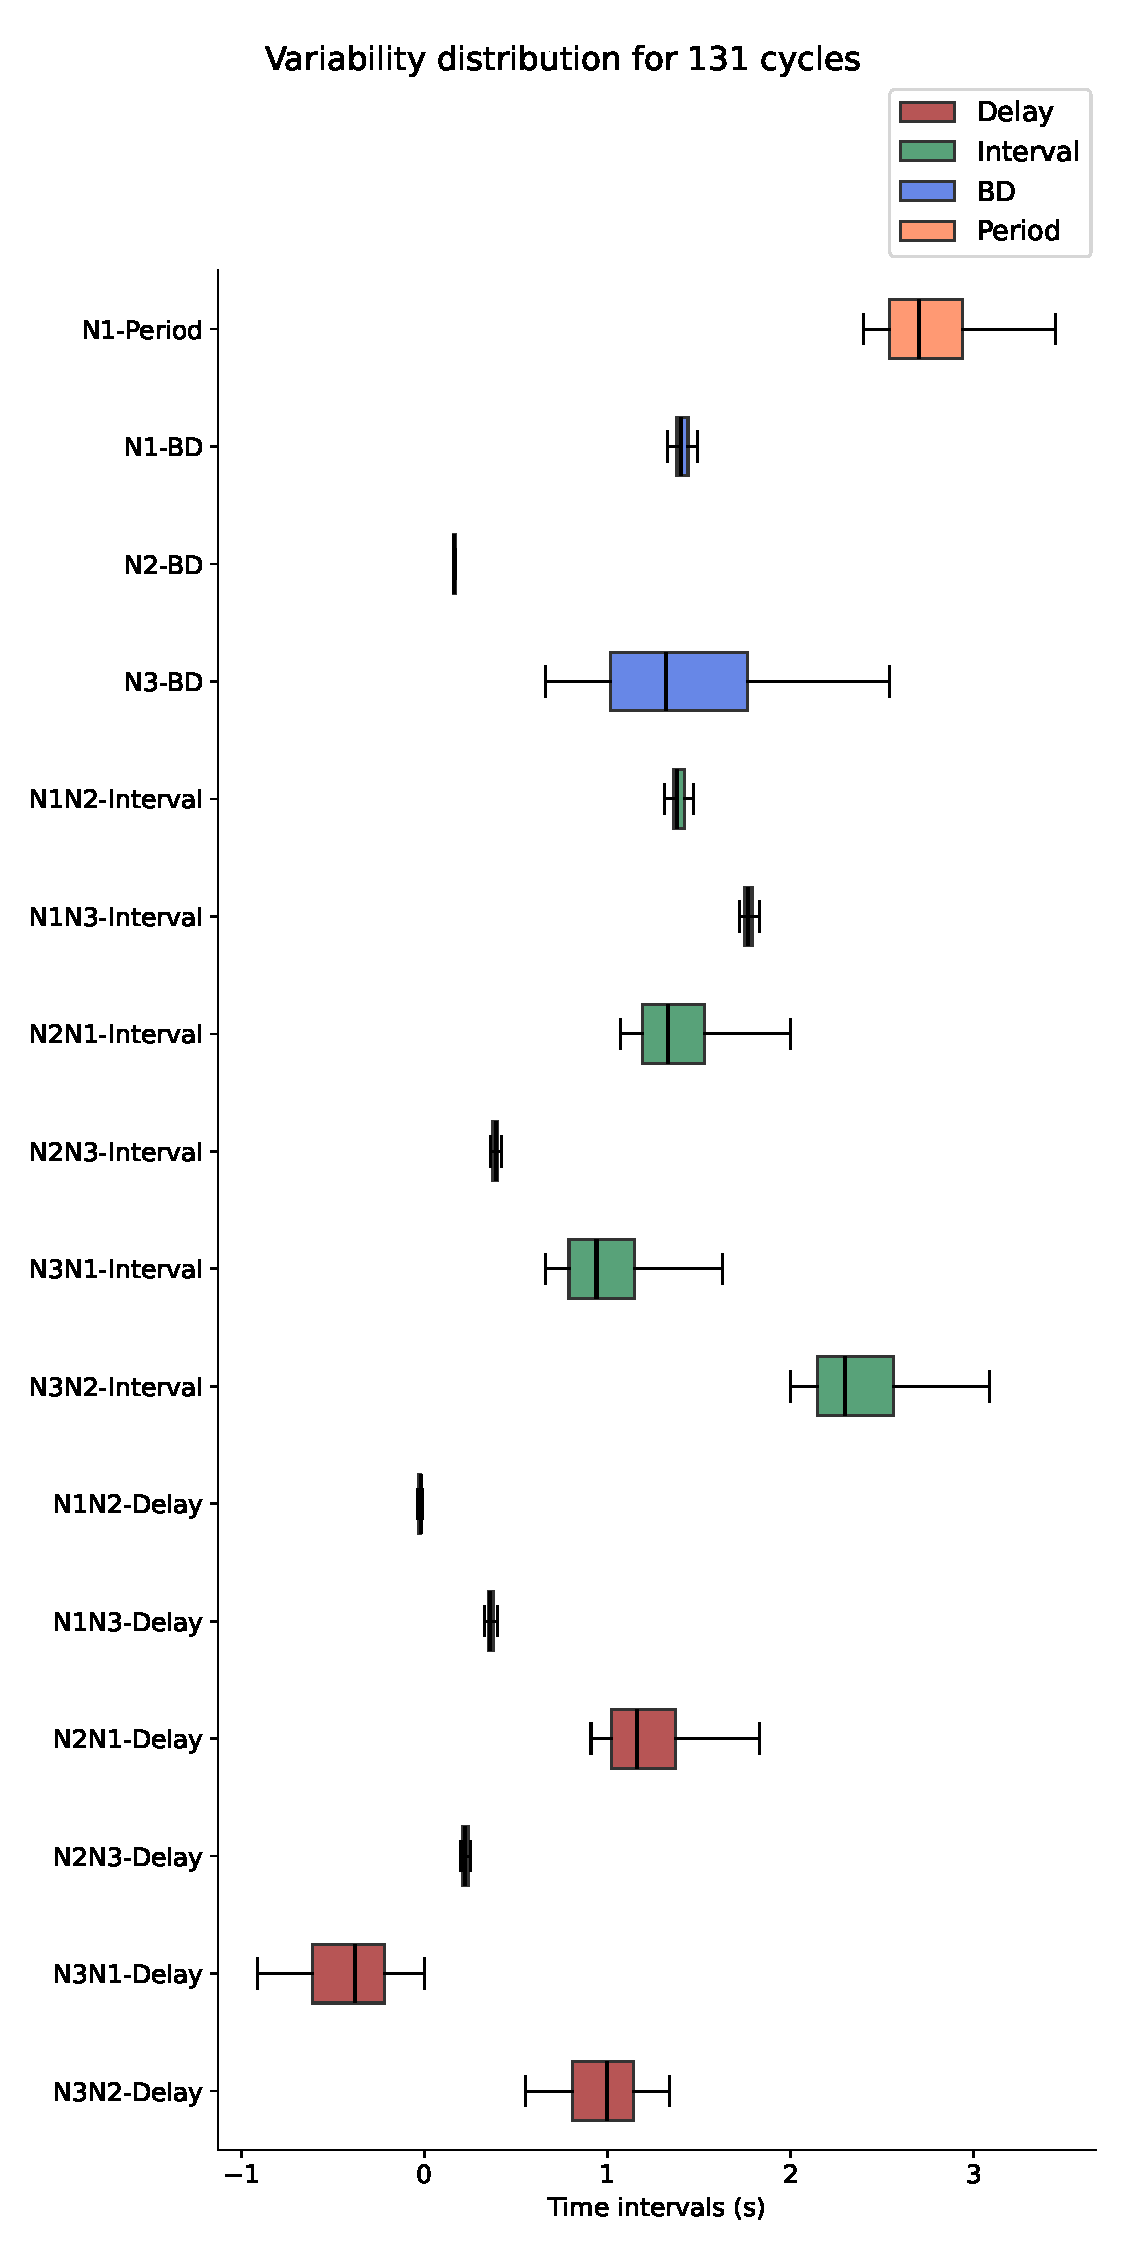
\includegraphics[width=\textwidth]{invariants/data/MODEL/n3t_driven/images/3phases/_boxplot.pdf}
	\end{minipage}
	\begin{minipage}[b]{0.53\textwidth}
		\centering
		\begin{minipage}[b]{\textwidth}
			\centering
			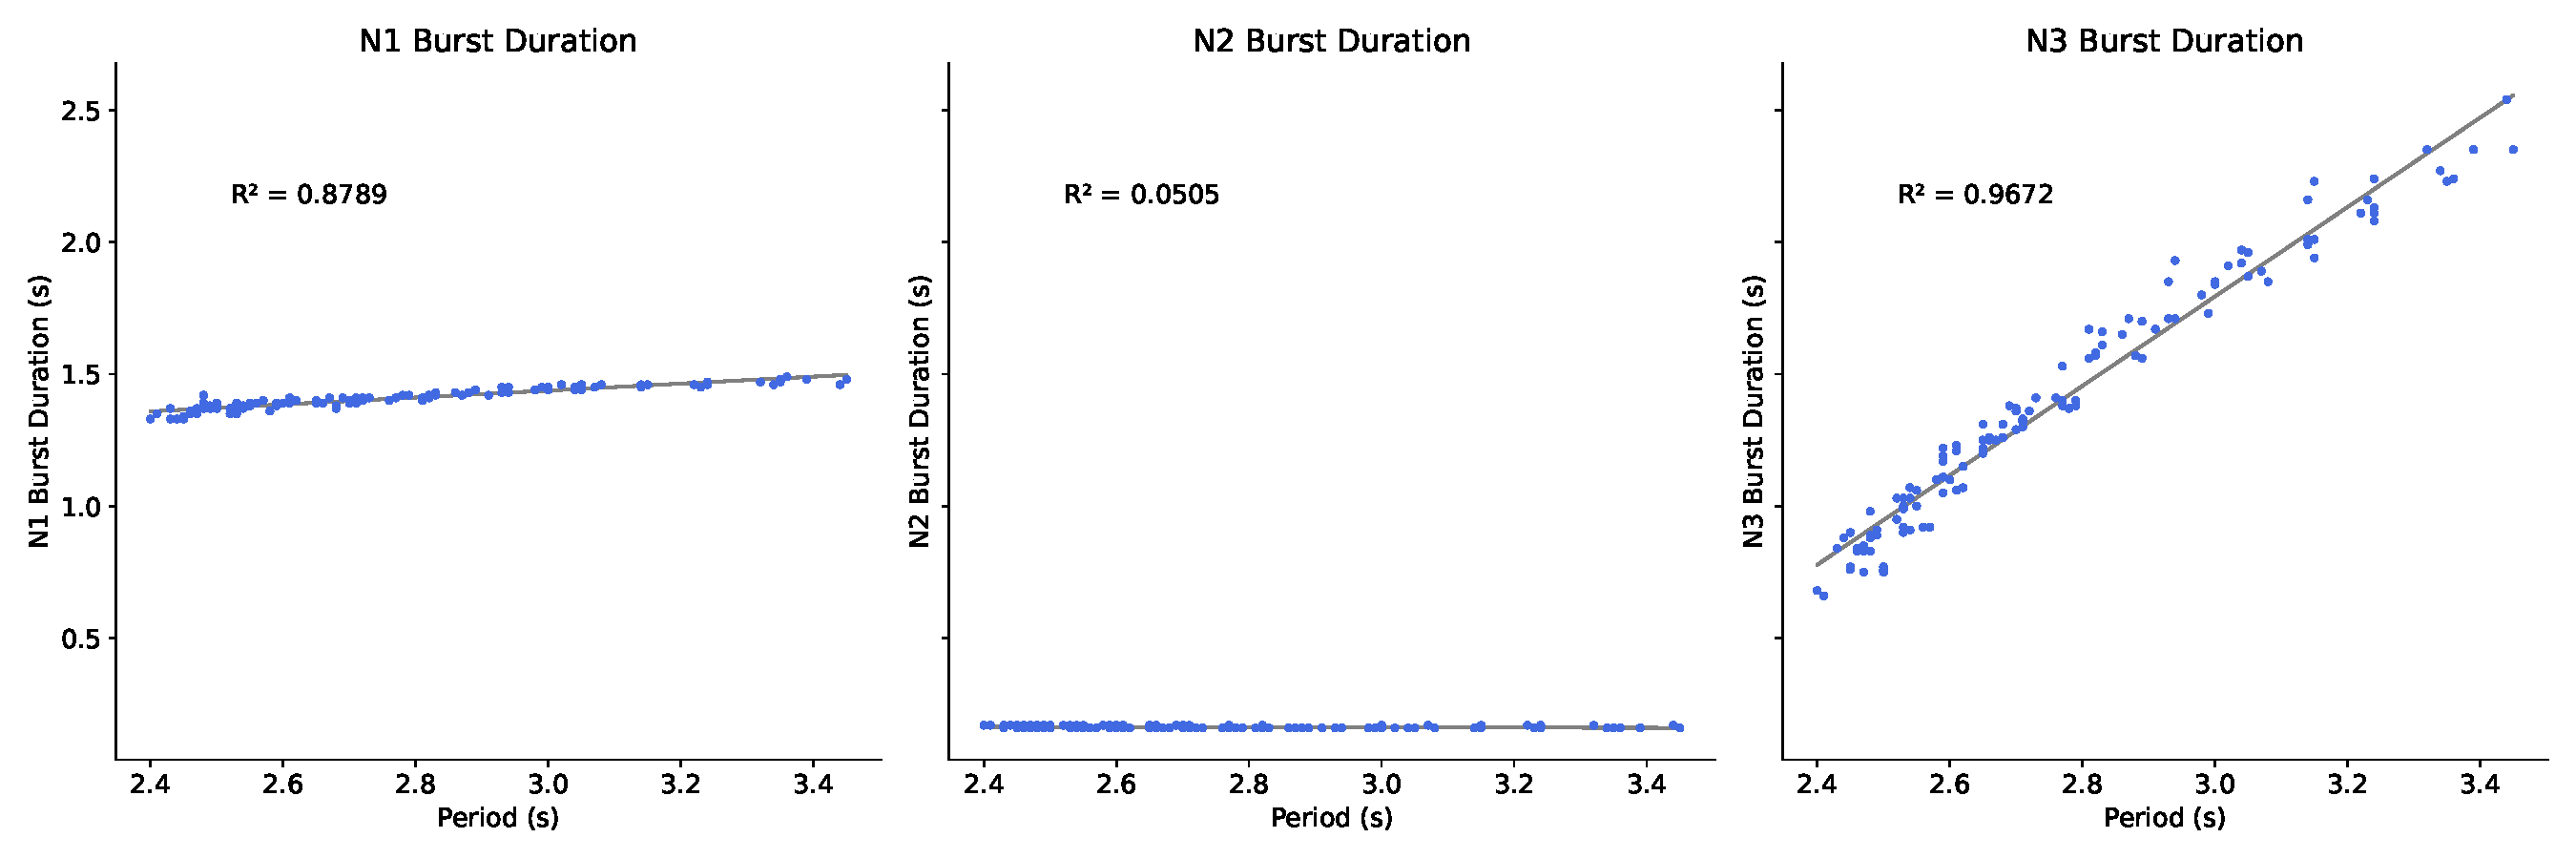
\includegraphics[width=\textwidth]{invariants/data/MODEL/n3t_driven/images/3phases/_durations.pdf}
		\end{minipage}\
		\begin{minipage}[b]{\textwidth}
			\centering
			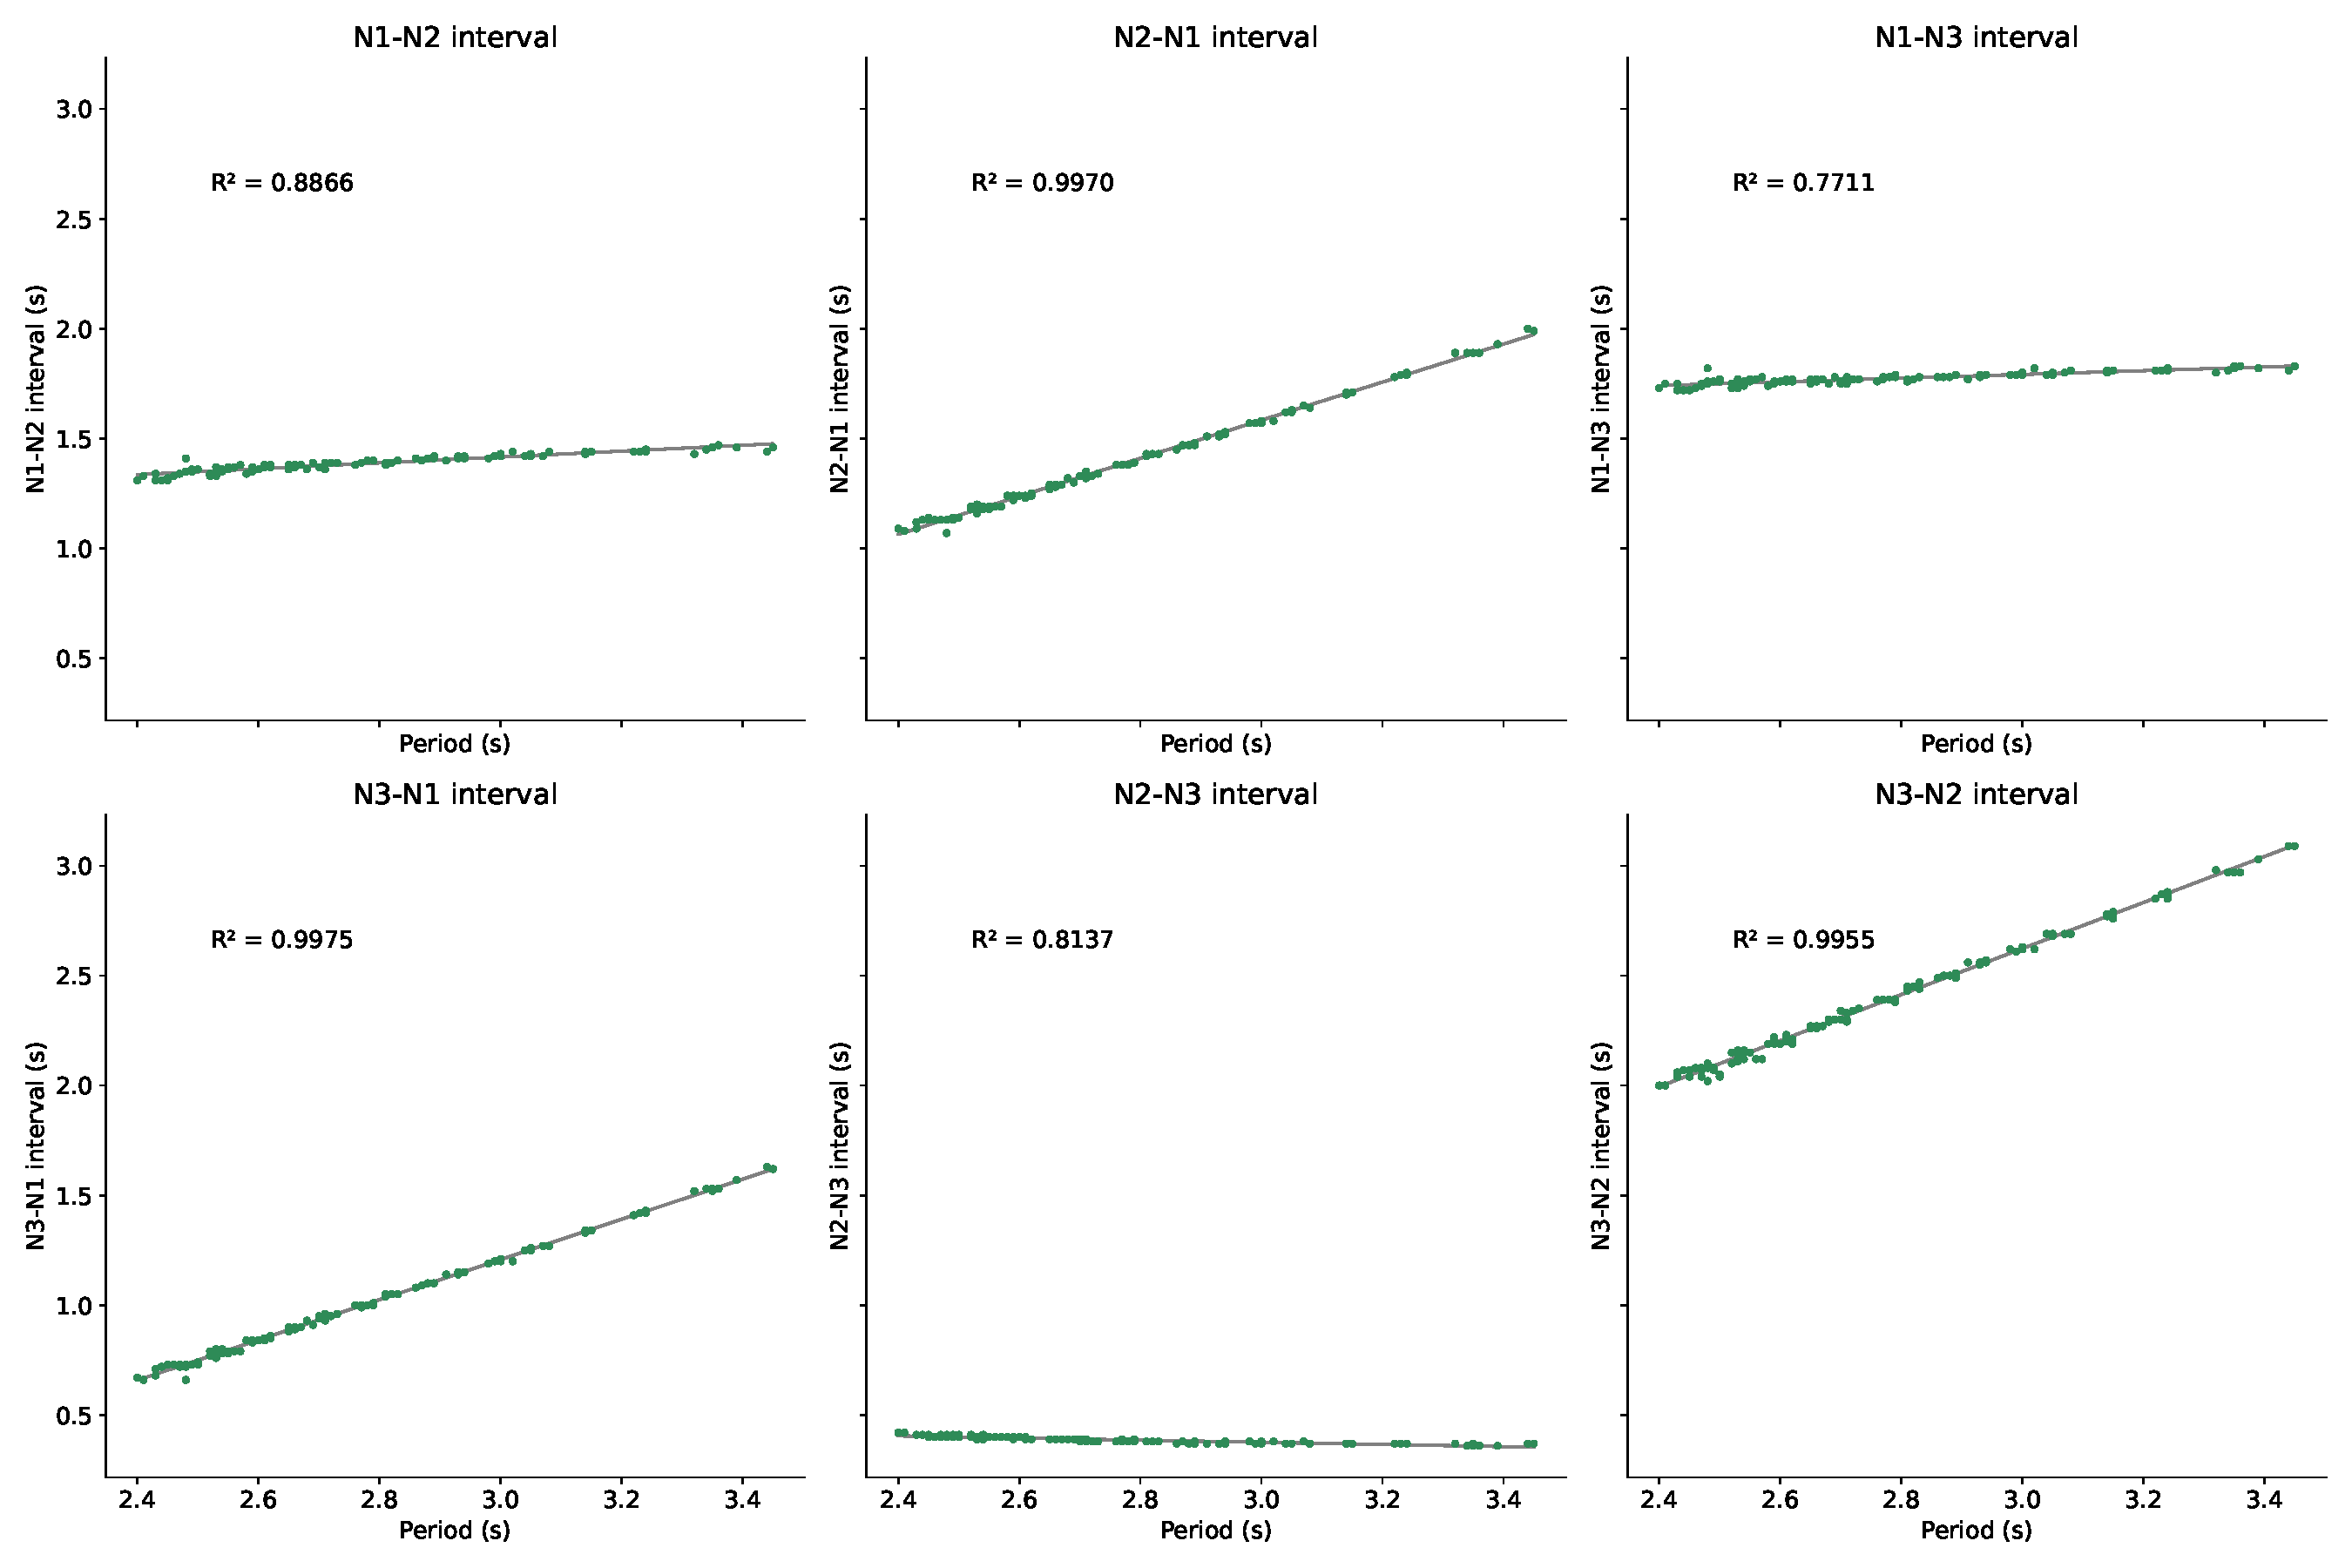
\includegraphics[width=\textwidth]{invariants/data/MODEL/n3t_driven/images/3phases/_intervals.pdf}
		\end{minipage}\
		\begin{minipage}[b]{\textwidth}
			\centering
			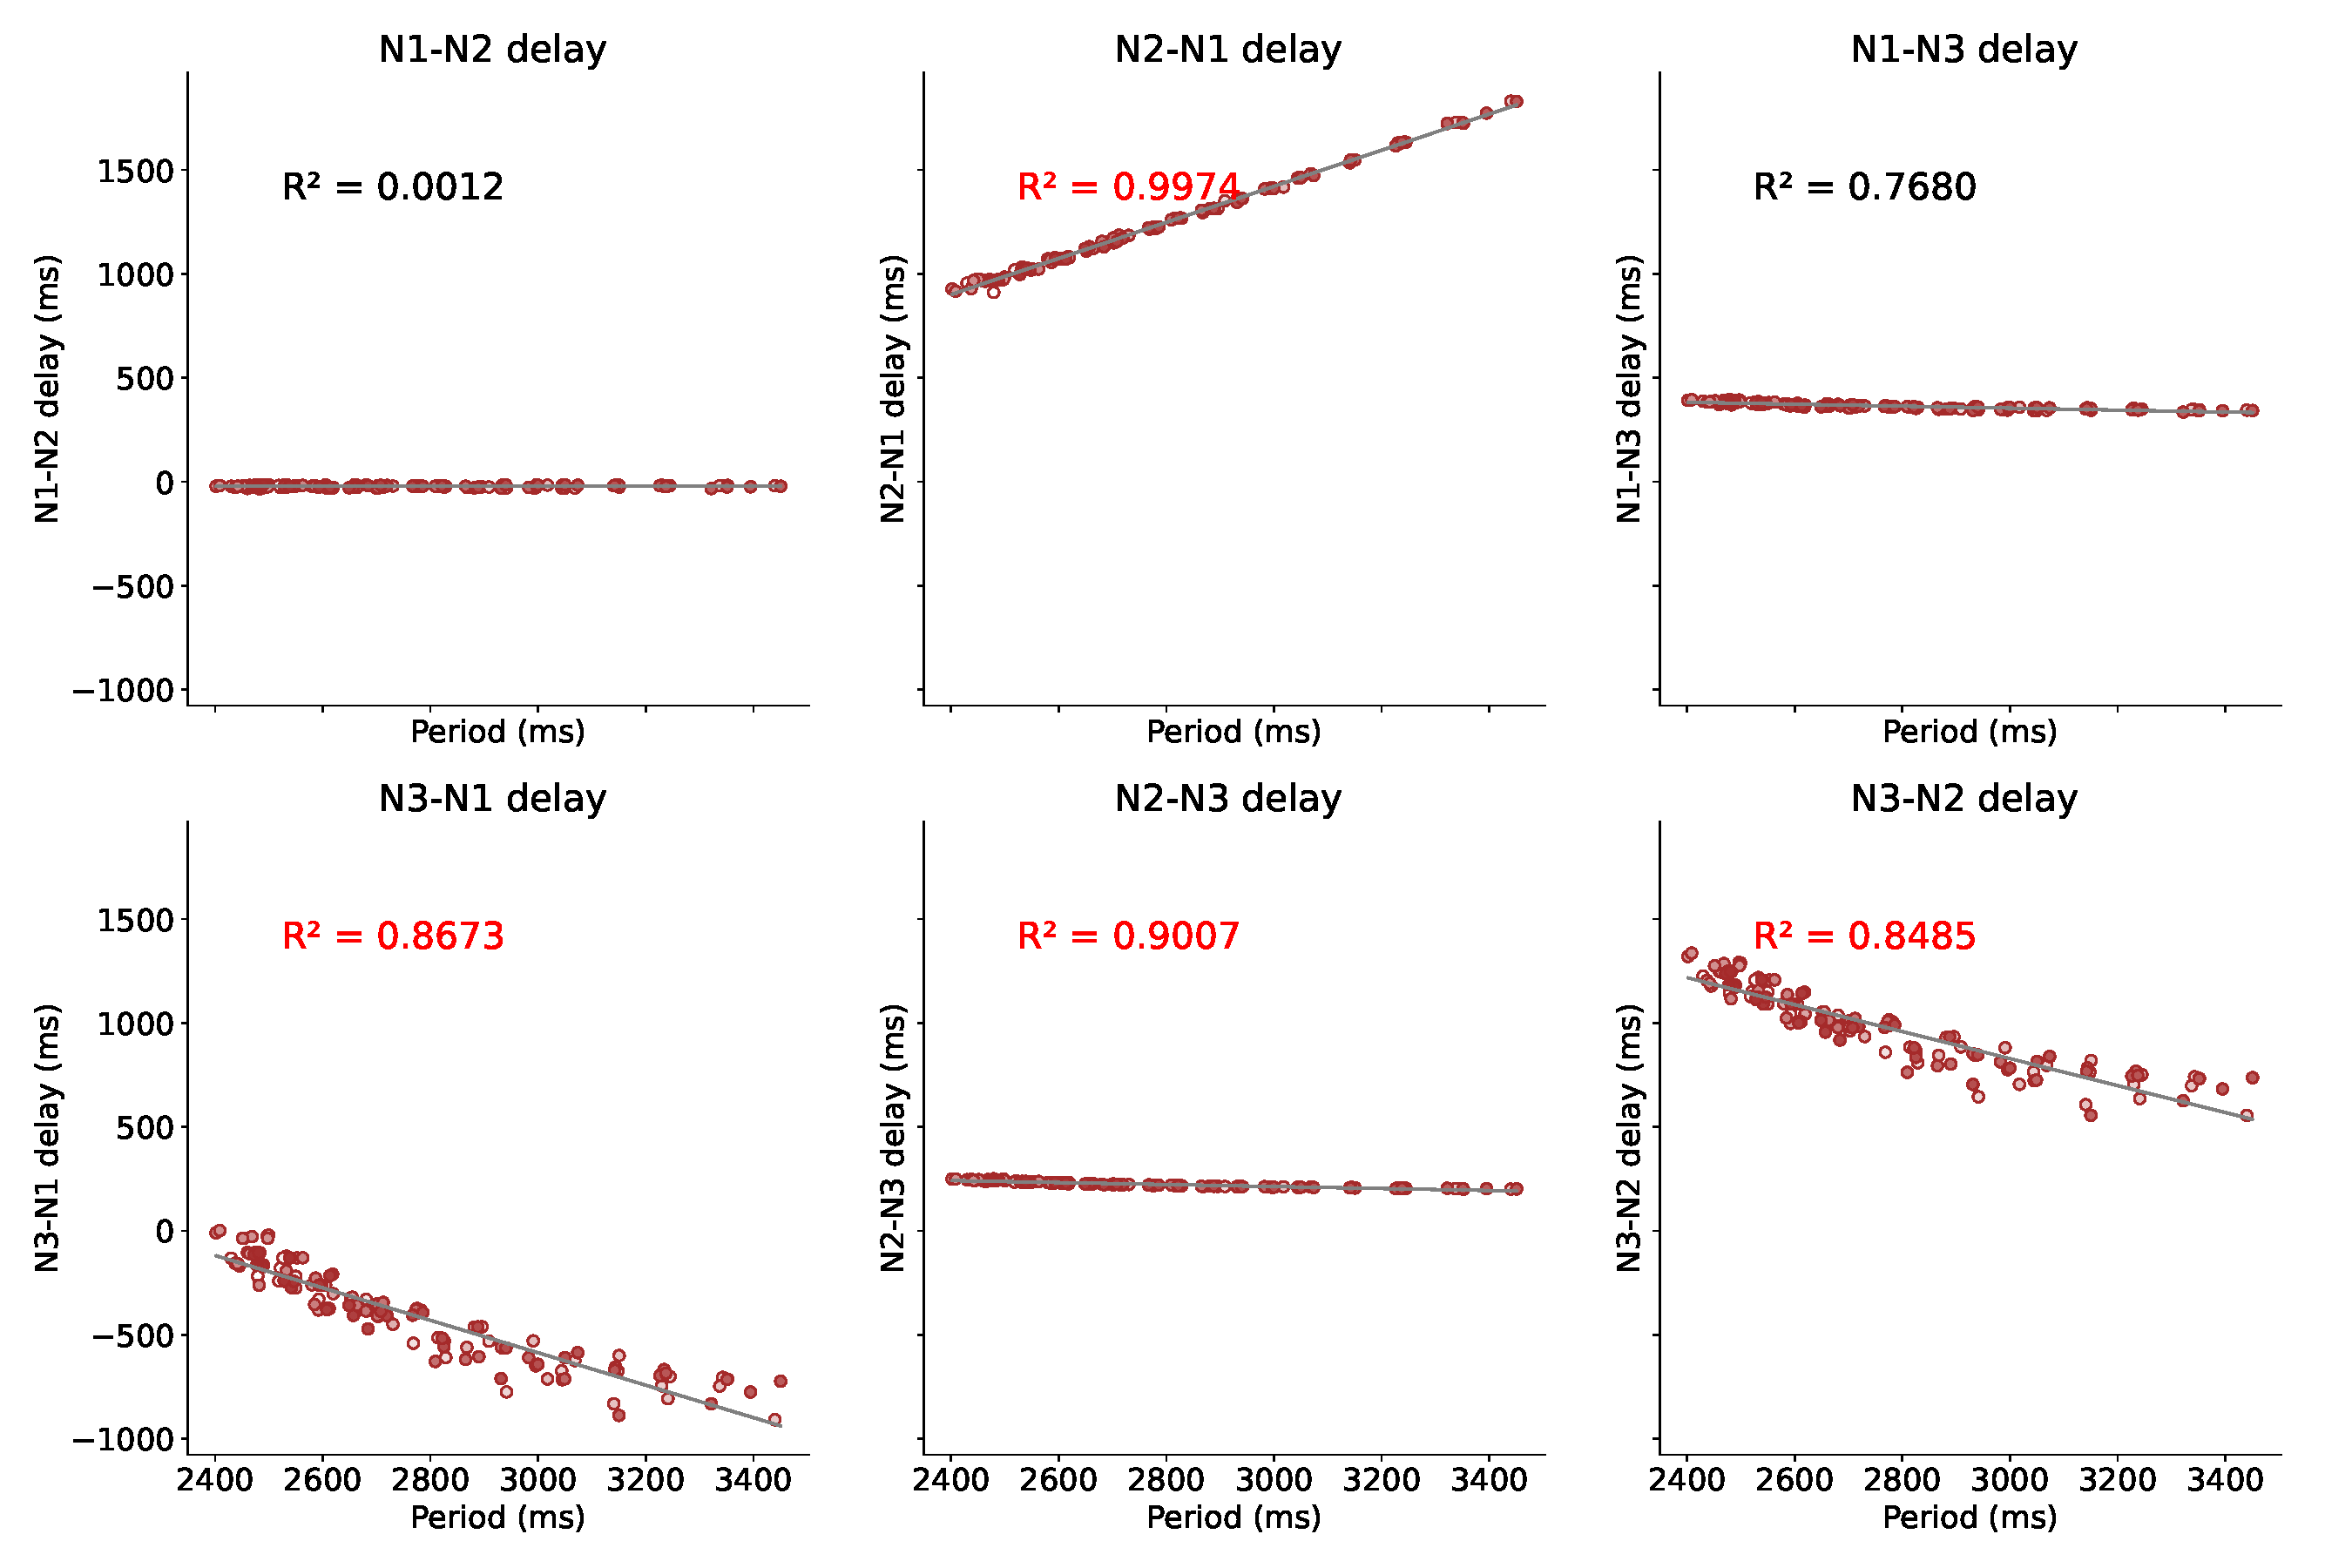
\includegraphics[width=\textwidth]{invariants/data/MODEL/n3t_driven/images/3phases/_delays.pdf}
		\end{minipage}
	\end{minipage}
	\caption{\textbf{N3t stimulation:} a) Box-plots of the sequence intervals under N3t neuron stimulation. b) Interval correlations to Period for N3t-driven simulation. First row: Burst duration. Second and third row: Two-neuron intervals. Forth and fifth row: Two-neuron delays.}
	\label{fig:invariants n3t}
\end{figure}





\subsection{SO driven variability}
\label{subsec:so driven}

The same protocol was implemented with a ramp stimulation applied to SO to induce variability, using the injected current values shown in Table \ref{table:inj values} for each neuron. Events were detected and all intervals were measured (Fig. \ref{fig:intervals}) and their variability was characterized. %This neuron has also been used in previous studies with stimulation protocols both in electrophysiological experiments and in model simulations due to its important role in rhythm activation and modulation. ***se podría quitar, si no hay que poner las referencias otra vez****

\begin{figure}[hbt!]
	\begin{minipage}[b]{0.45\textwidth}
		\centering
		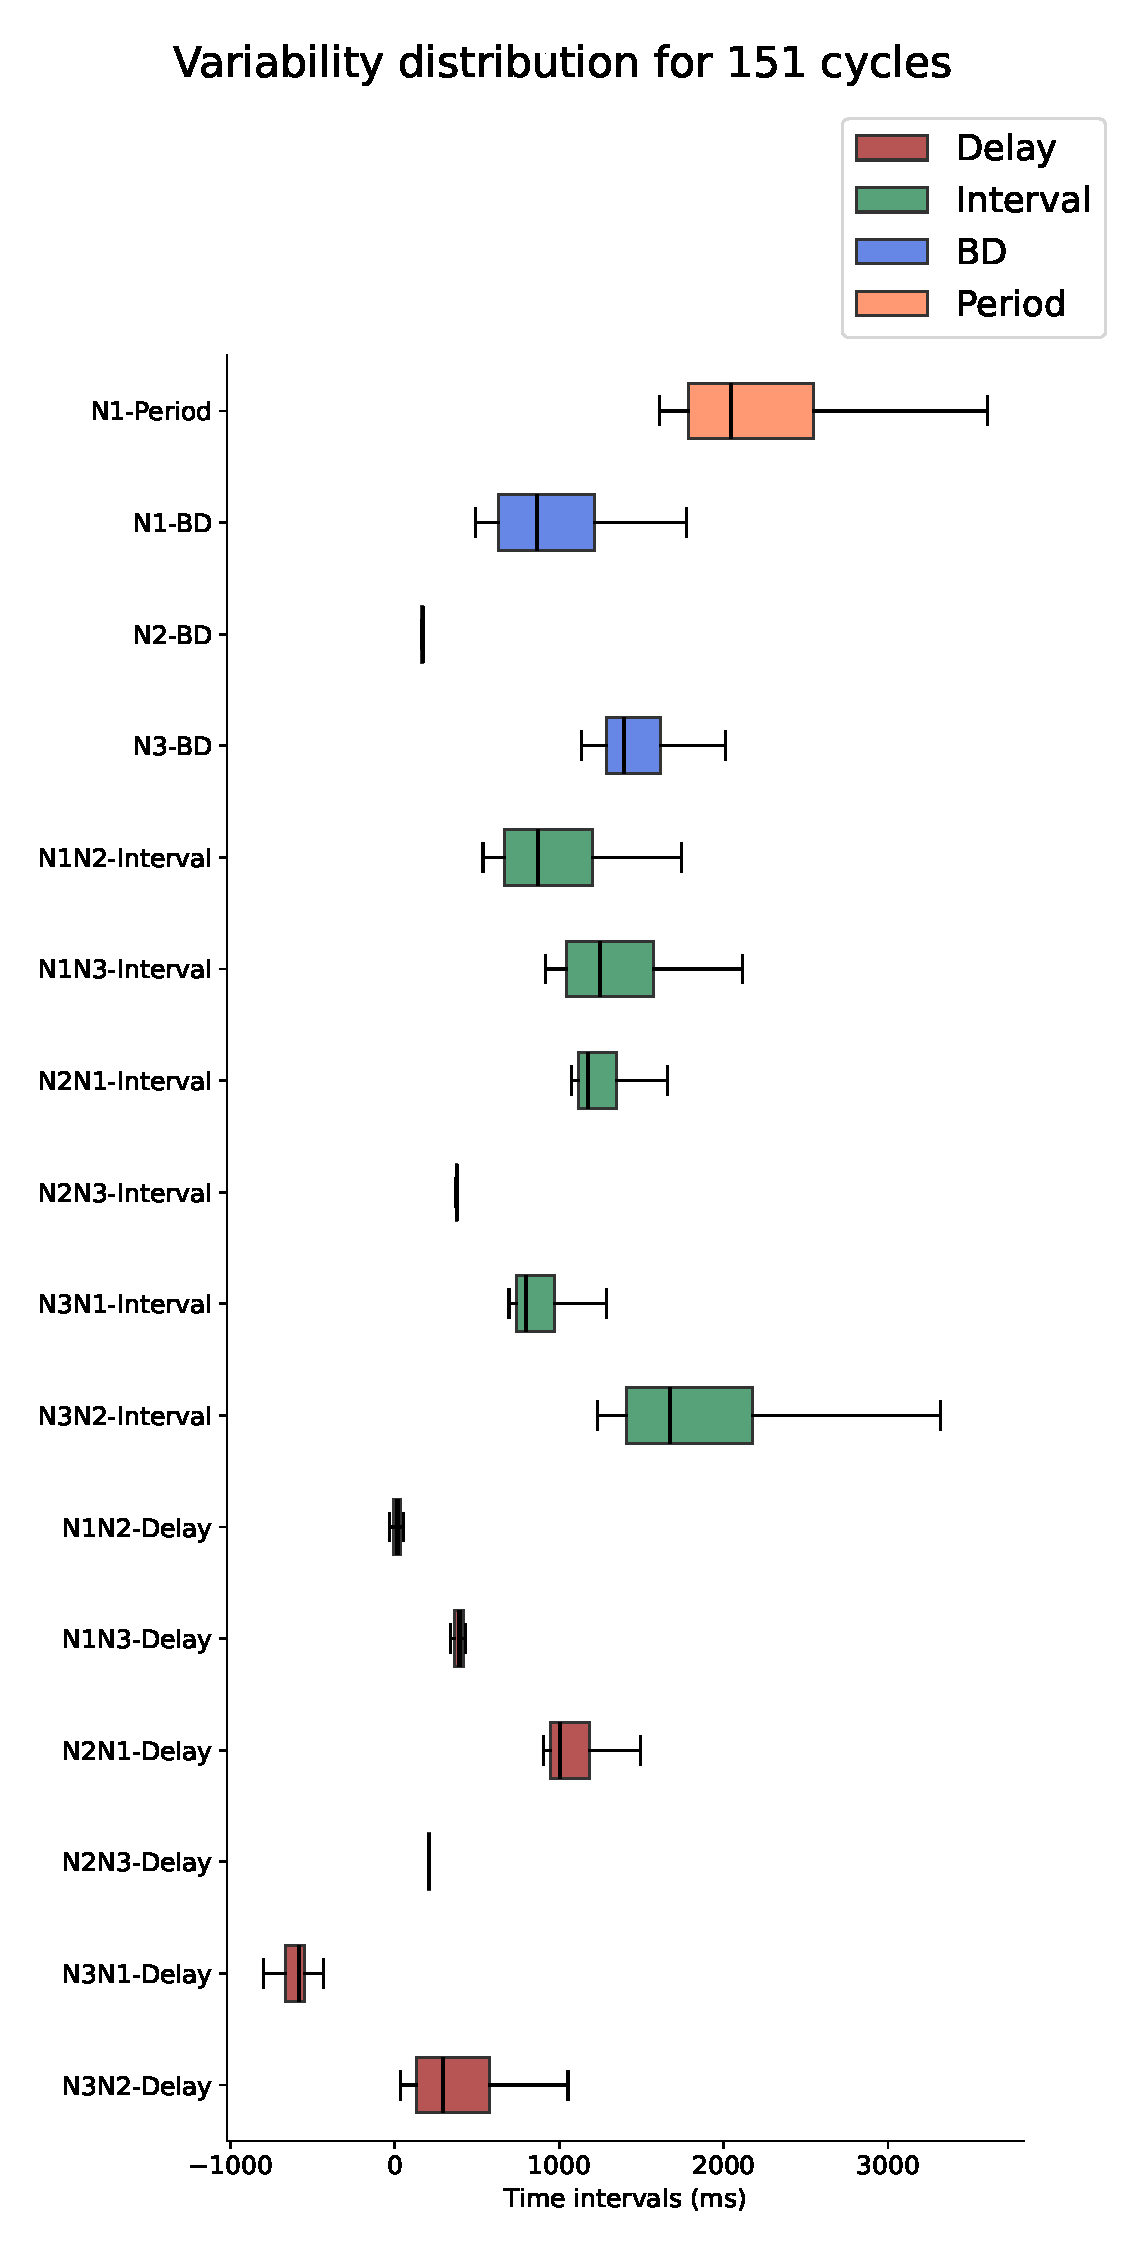
\includegraphics[width=\textwidth]{invariants/data/MODEL/so_driven/images/3phases/_boxplot.pdf}
	\end{minipage}
	\begin{minipage}[b]{0.53\textwidth}
		\centering
		\begin{minipage}[b]{\textwidth}
			\centering
			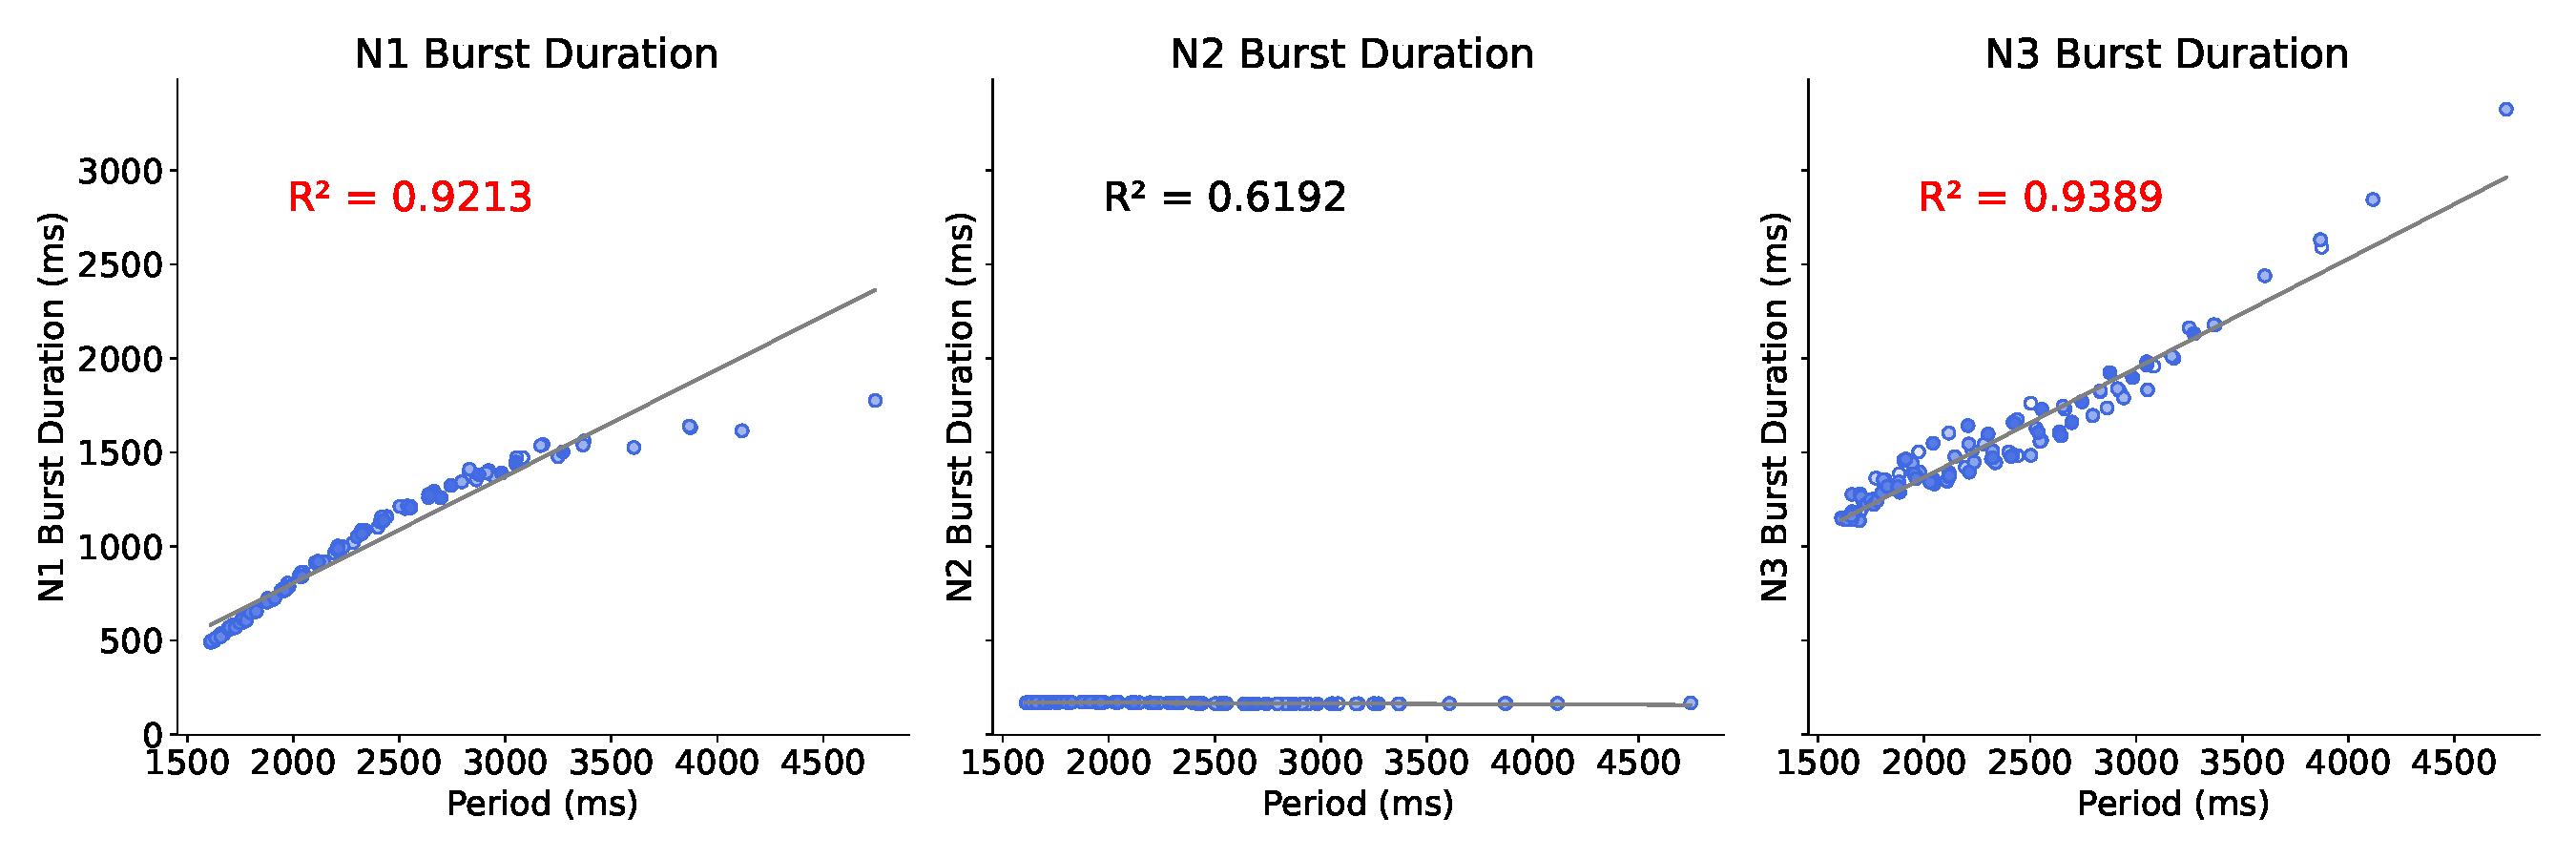
\includegraphics[width=\textwidth]{invariants/data/MODEL/so_driven/images/3phases/_durations.pdf}
		\end{minipage}\
		\begin{minipage}[b]{\textwidth}
			\centering
			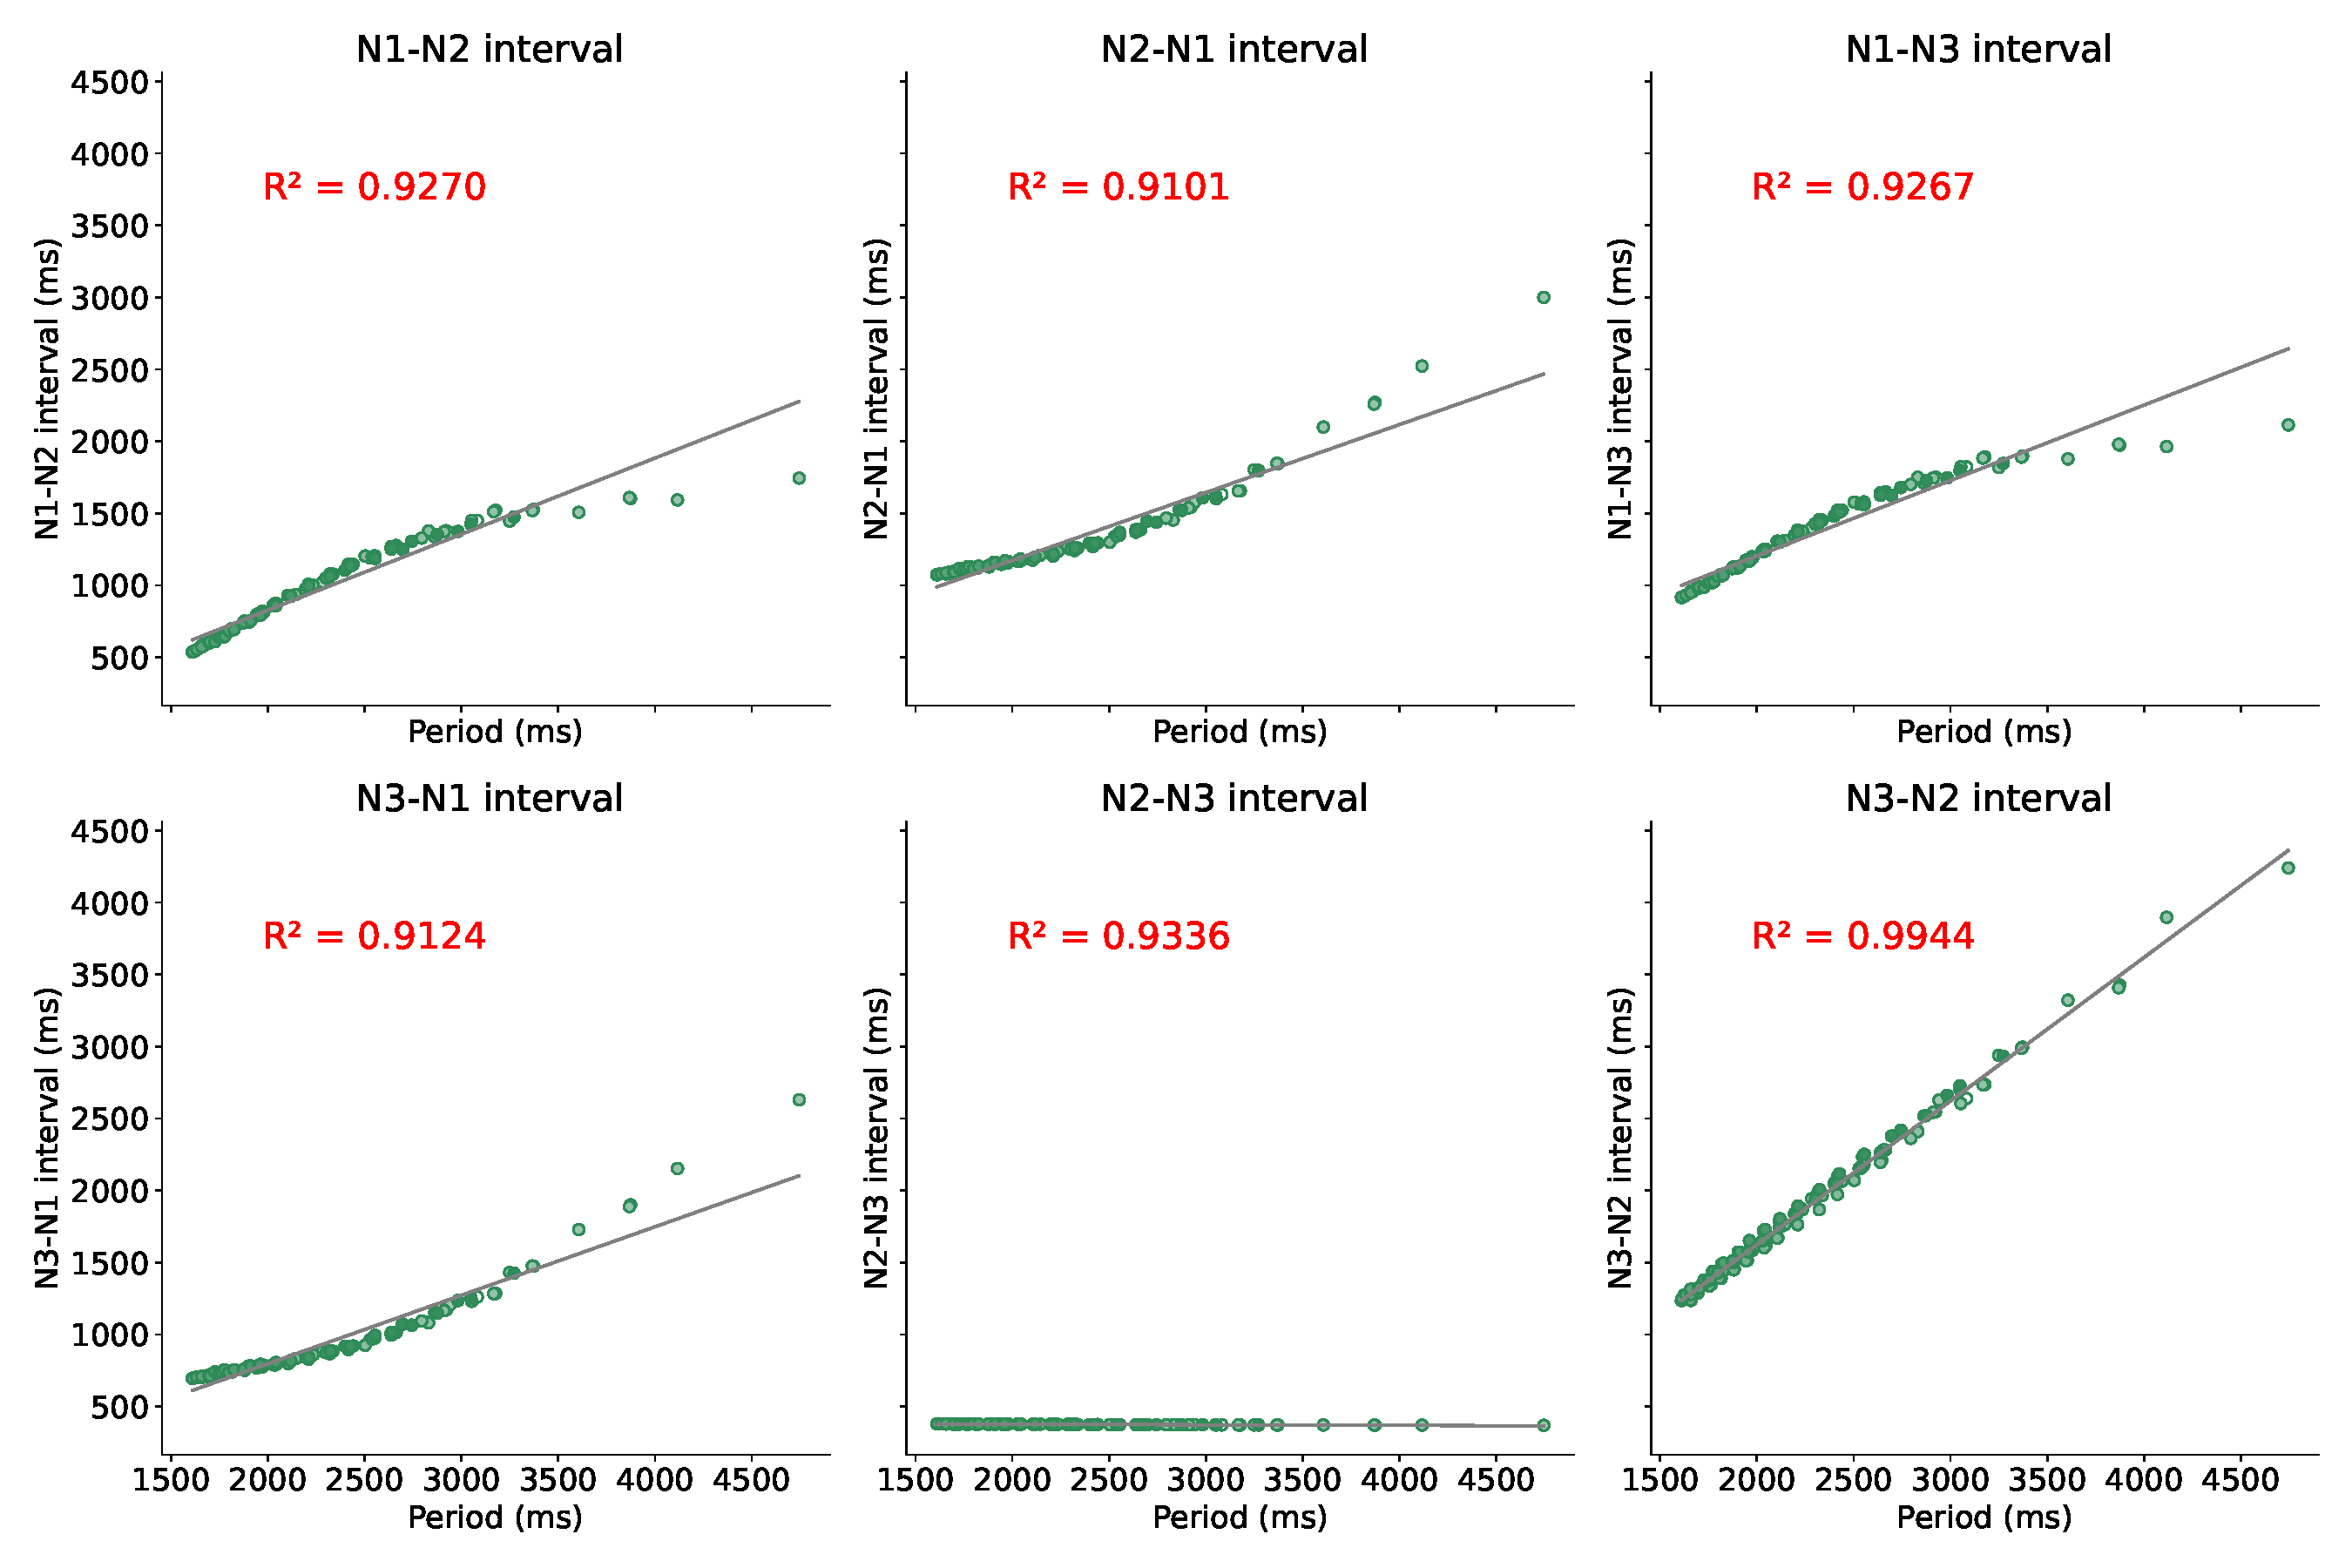
\includegraphics[width=\textwidth]{invariants/data/MODEL/so_driven/images/3phases/_intervals.pdf}
		\end{minipage}\
		\begin{minipage}[b]{\textwidth}
			\centering
			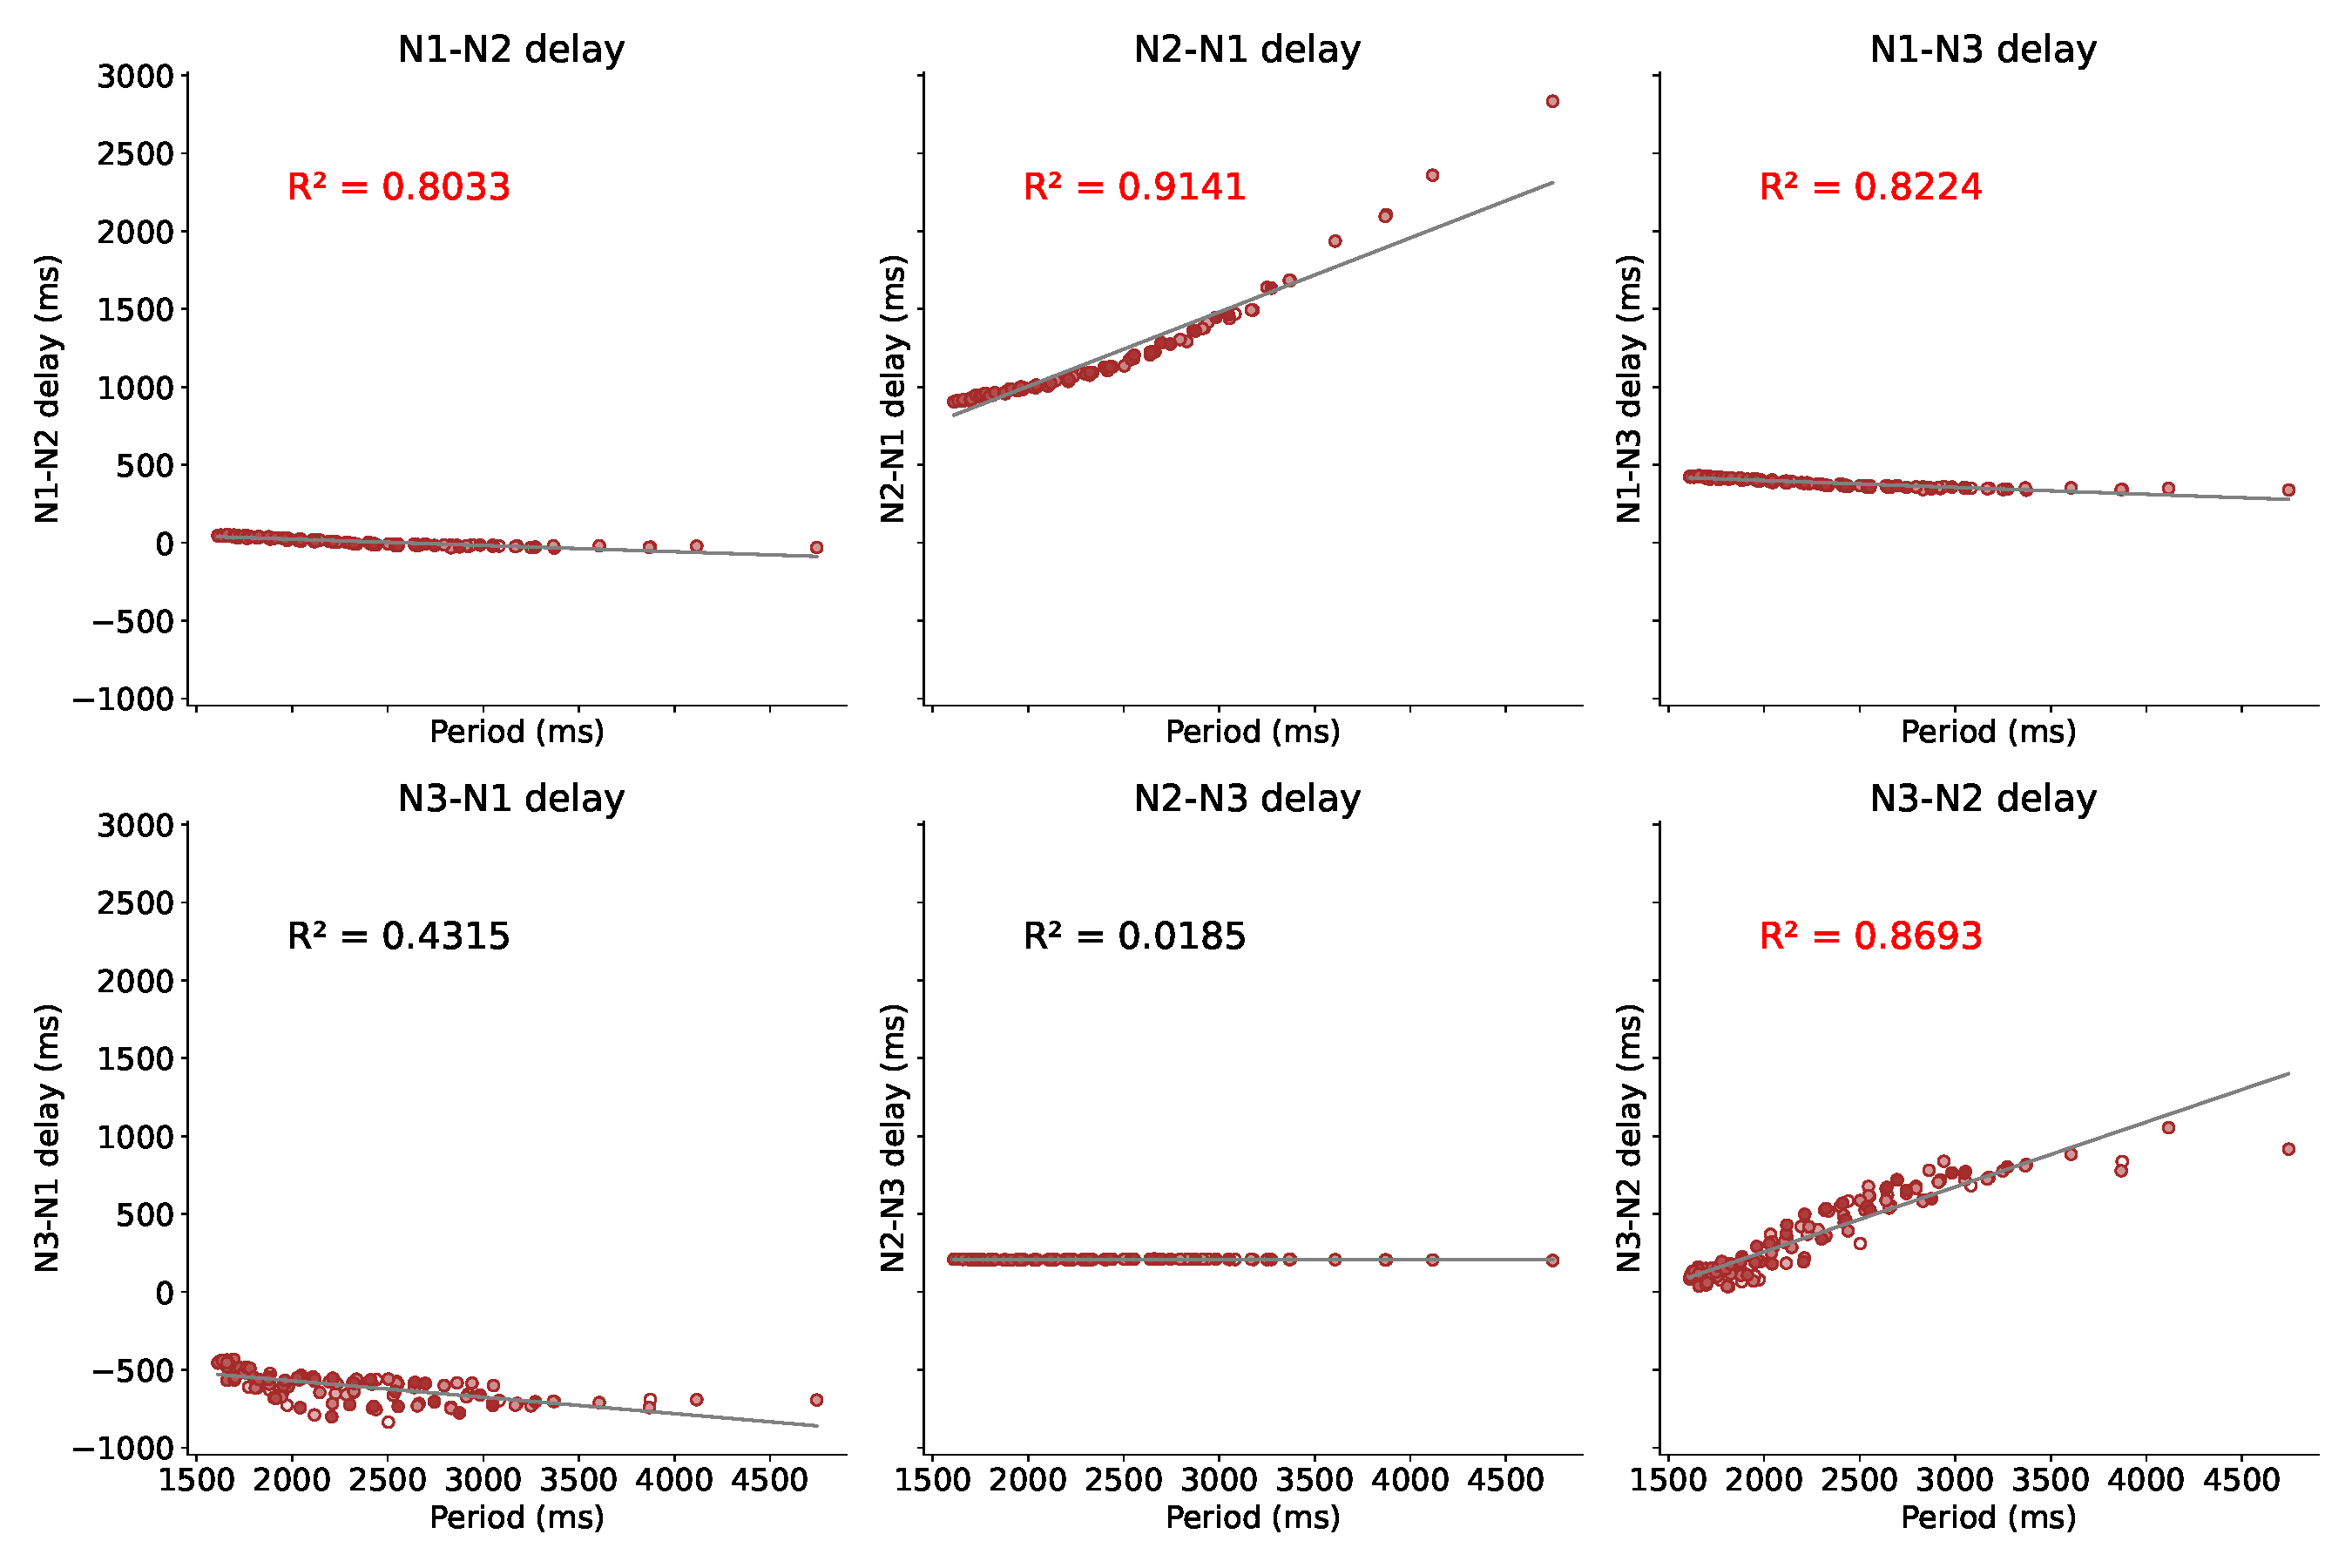
\includegraphics[width=\textwidth]{invariants/data/MODEL/so_driven/images/3phases/_delays.pdf}
		\end{minipage}
	\end{minipage}
	\caption{\textbf{SO stimulation: }a) Box-plots of the sequence intervals under SO neuron stimulation. b) Interval correlations to Period for SO-driven simulation. First row: Burst duration. Second and third row: Two-neuron intervals. Forth and fifth row: Two-neuron delays.}
	\label{fig:invariant so}
\end{figure}


Figure \ref{fig:invariant so}.a) displays the box-plot representing the distinct interval variability. In this case, we found more intervals showing large variability than in the previous cases. N2v intervals, as it happened in the previous results, show low variability. %, which indicates that period variability is more likely a consequence of N3t and N1M activity.
N1M and N3t neurons show high variability in their burst duration intervals, being N1M even more variable than N3t, as opposed to the previous results when the stimulation was introduced in other cells. All intervals derived from these two neurons have high variability and a similar structure. %Therefore, now the intervals which show low variability are the ones related to N2v. 

% In spite all this, what remains constant from N1M-driven simulation is the variability of the N3-N2 interval, which includes both N1M and N3t burst duration, being N3-N2 the most variable one, and the closest to the period variability.%distribution

% Since in this case there are more neurons showing high variability, we should expect finding more correlations when plotting each interval against the period.  ***también deberíamos quitar redundancia aquí***
% Hence, as it happened in the previous results, all intervals related to N3t show dynamical invariants, but this time they are also present in the ones related with N1M, which show a high variability. 
% the intervals with more variability and, thus, those that had a more similar variability structure to the period, were the ones that showed dynamical invariants%(a highest linear relation to the period)


Figure \ref{fig:invariant so}.b) displays the corresponding correlation analysis between all intervals and the period. %In this case, as it happens in the box-plot, there are found different results
In this case, we found correlations in the same intervals as before: N2-N1, N3-N1, N3-N2 intervals and N2-N1 delay; which are the intervals related to N3t burst duration. However, under SO stimulation,  N1-N2, N1-N3 intervals were also highly correlated to the period. Even the correlation for N3-N2 delay considerably increased in relation to the other stimulation conditions. These intervals are the ones related to N1M neuron activity, and were also the most variable ones.  These results reproduce the experimentally analyzed effects set out in \parencite{Elliott1991}, when rhythm and variability was induced by injecting current into a living SO neuron.

%Furthermore, it is important to notice that N3-N1 delay is negative again ****por qué es importante si es lo mismo que antes****. As it happened in N3t-driven simulation, this means there is a constant overlapping between N3 and N1 in each cycle, i.e. N3t burst interval is coming earlier. This can be also appreciated in boxplot, since this interval is represented below 0. 

Compared to the N1M and N3t stimulation results, there is another difference when driving the rhythm with SO: burst duration is much shorter, so the period and the rest of intervals are consequently smaller. Therefore, when driving the rhythm by SO, the period variability seems to arise from both N3t as well as by N1M. 
%the model produces a rhythm where the information about period duration seems to be carried by N3t as well as by N1M. 



\subsection{Time intervals relations cycle-by-cycle beyond period}
We saw so far the sequential dynamical invariants in terms of strong linear relationships between the distinct intervals in a cycle and the period, however, studying the relations between all possible combinations between intervals can also show interesting information about the temporal variability distribution in the ongoing activity. In Figs \ref{fig:model n1m stimulation pairplot} to \ref{fig:model so stimulation pairplot} there is a representation of all these combinations of the defined intervals for the three scenarios of induced variability (current in N1M, N3t or SO) showed in this section. In this extended representation of the relations cycle-by-cycle we can see that there are more intervals presenting strong linear relations, besides of the periods. Some of them are intervals that are contained in others, as the case of N1-BD and N1-N2 interval and have similar durations, and so they are more likely to have a strong linear relation between them. However, there are other intervals that, as it is the case of the period, although they share part of the time-interval, they are not correlated, since they are not the variable part, as it is the case of N2-BD with N1-N2. This disctintion can help disect the source of variability and its distribution when an interval is related to the period. Also, the further study of linear relation between some intervals (as N1-BD and N3-BD) that do not share time-interval, can show significant information about the ongoing activity cycle-by-cycle. This representation can also show non-linear relation between the intervals as we can see in some plots in the case of SO (Fig. \ref{fig:model so stimulation pairplot}), observed in the pyloric CPG in modeling and experimental scenarios \parencite{berbel_emergence_2024}.

\begin{figure}[htbp]
	\centering
	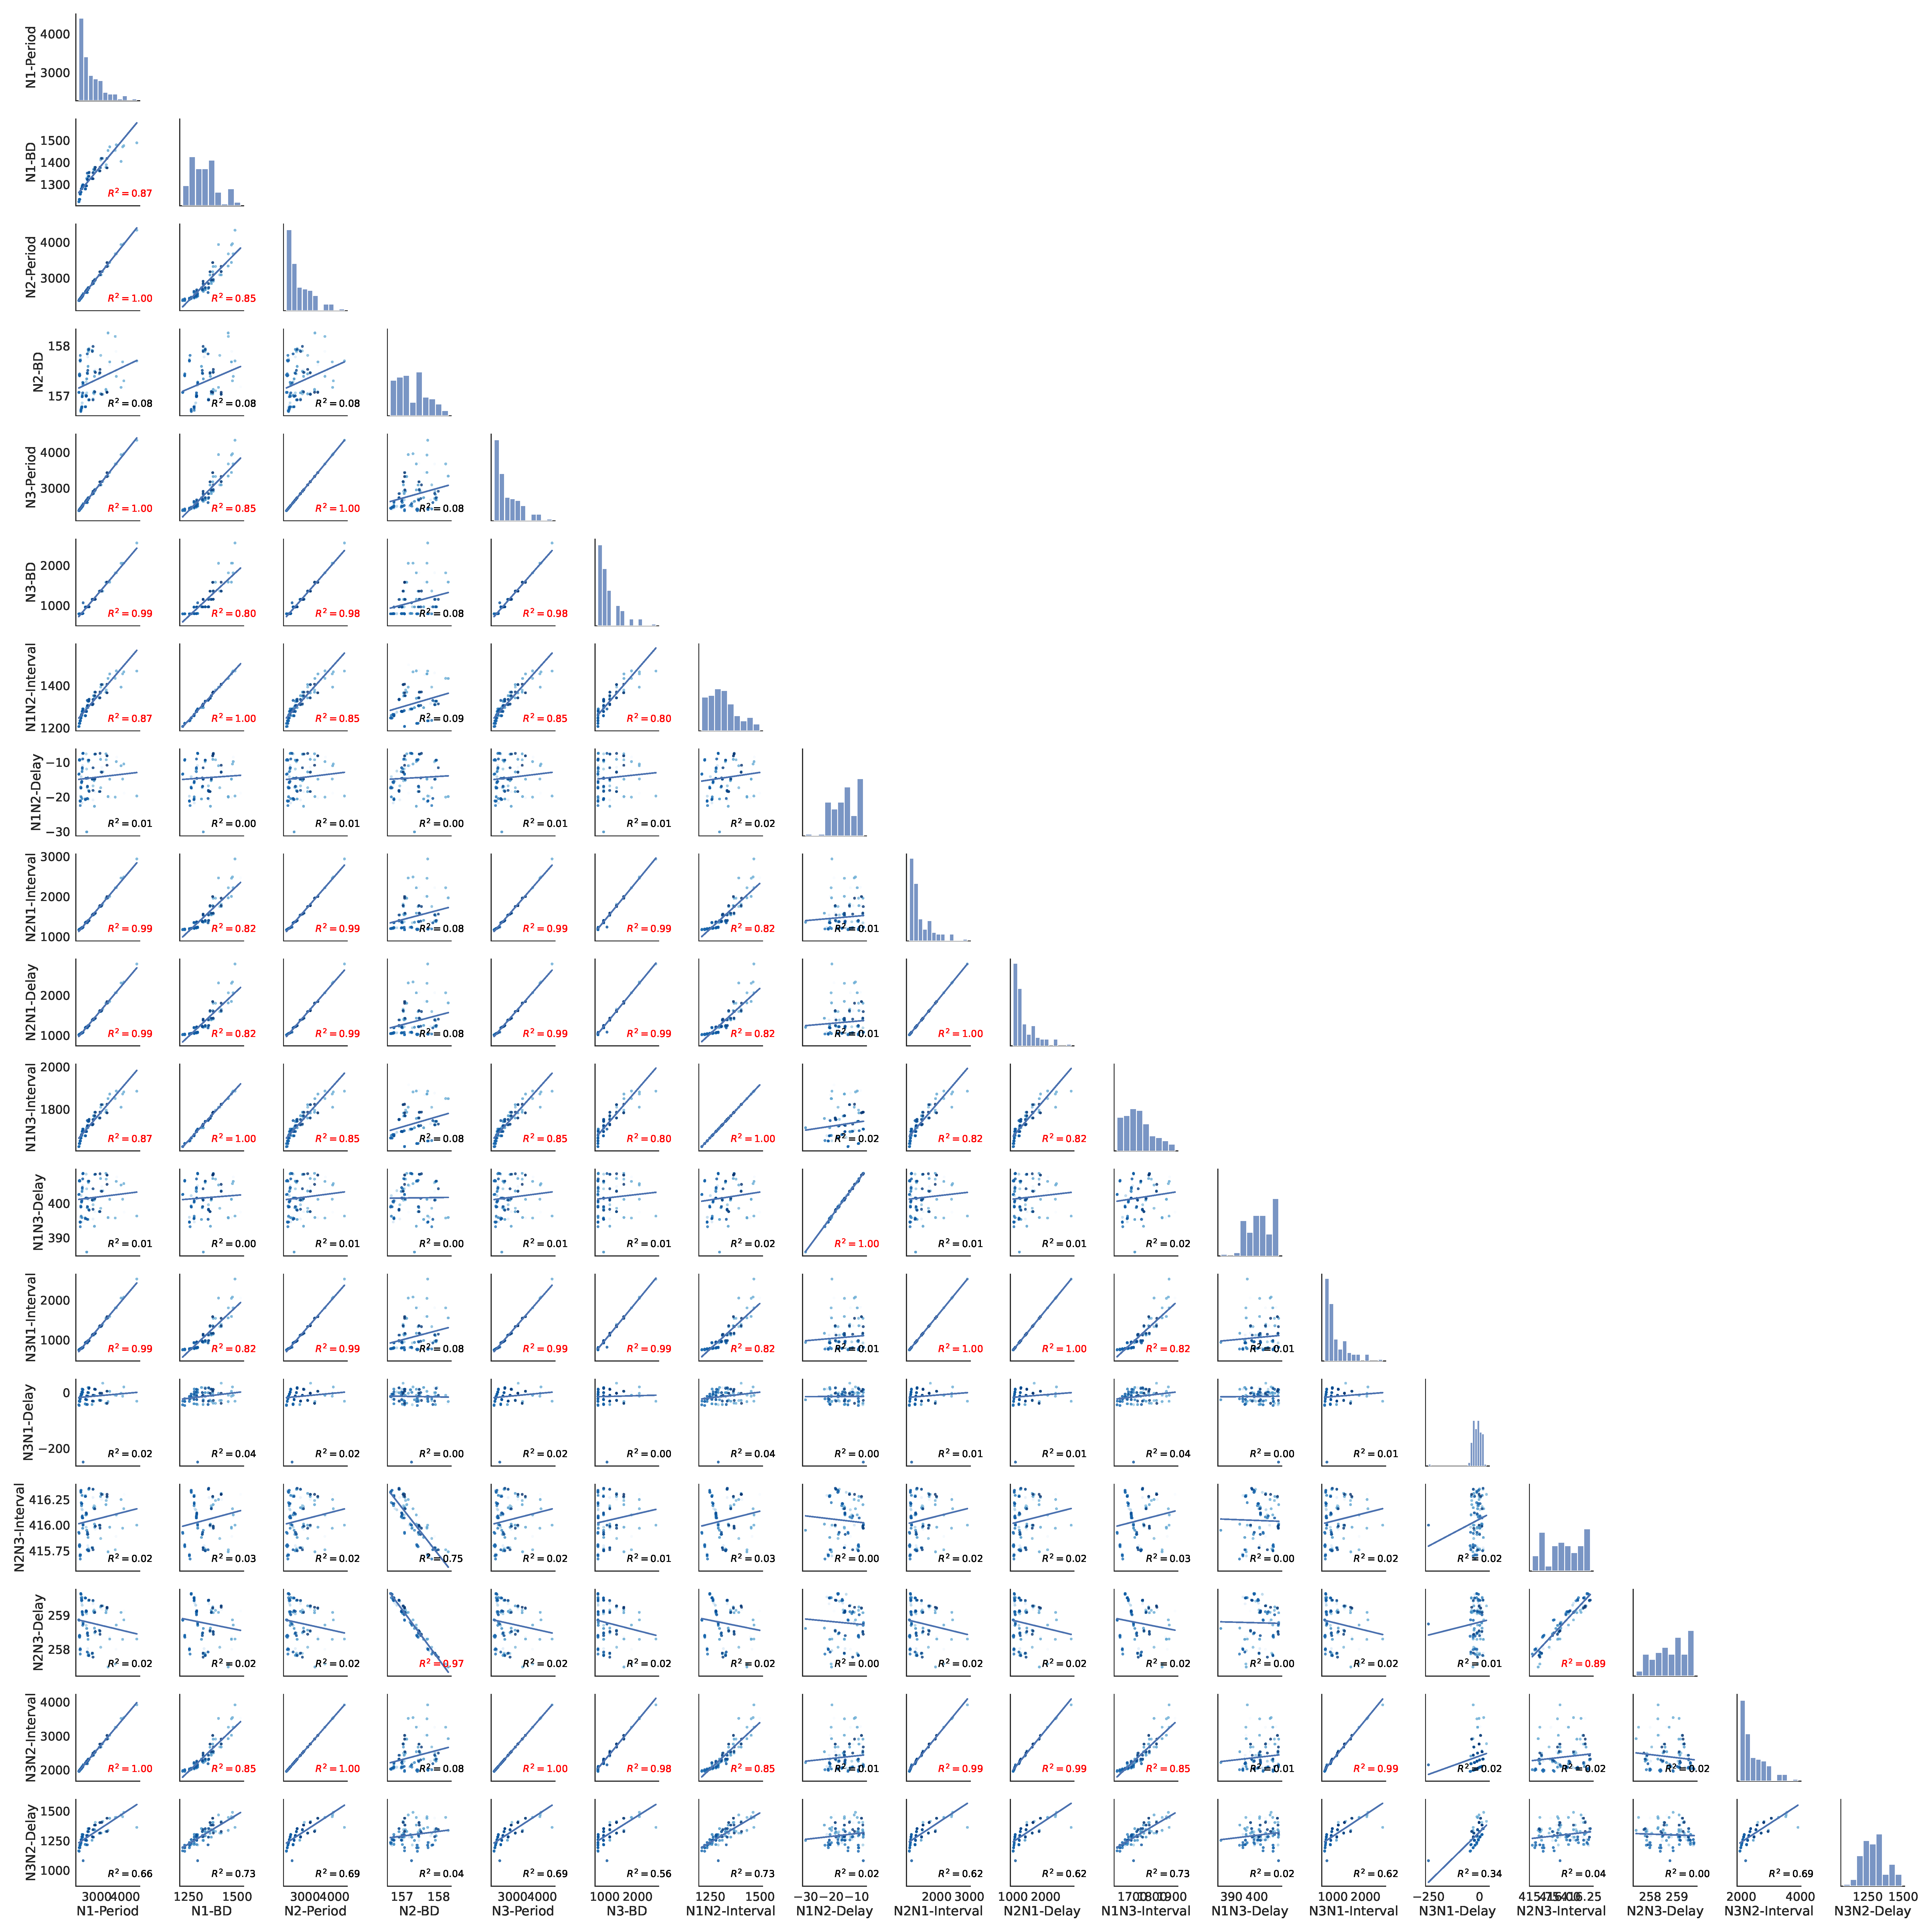
\includegraphics[width=\textwidth]{./invariants/data/MODEL/n1m_driven/images/3phases/output_pairplot.pdf}
	\caption{\textbf{N1M stimulation}: Pairplot with all possible combination between time intervals within a cycle.}
	\label{fig:model n1m stimulation pairplot}
\end{figure}
 
\begin{figure}[htbp]
	\centering
	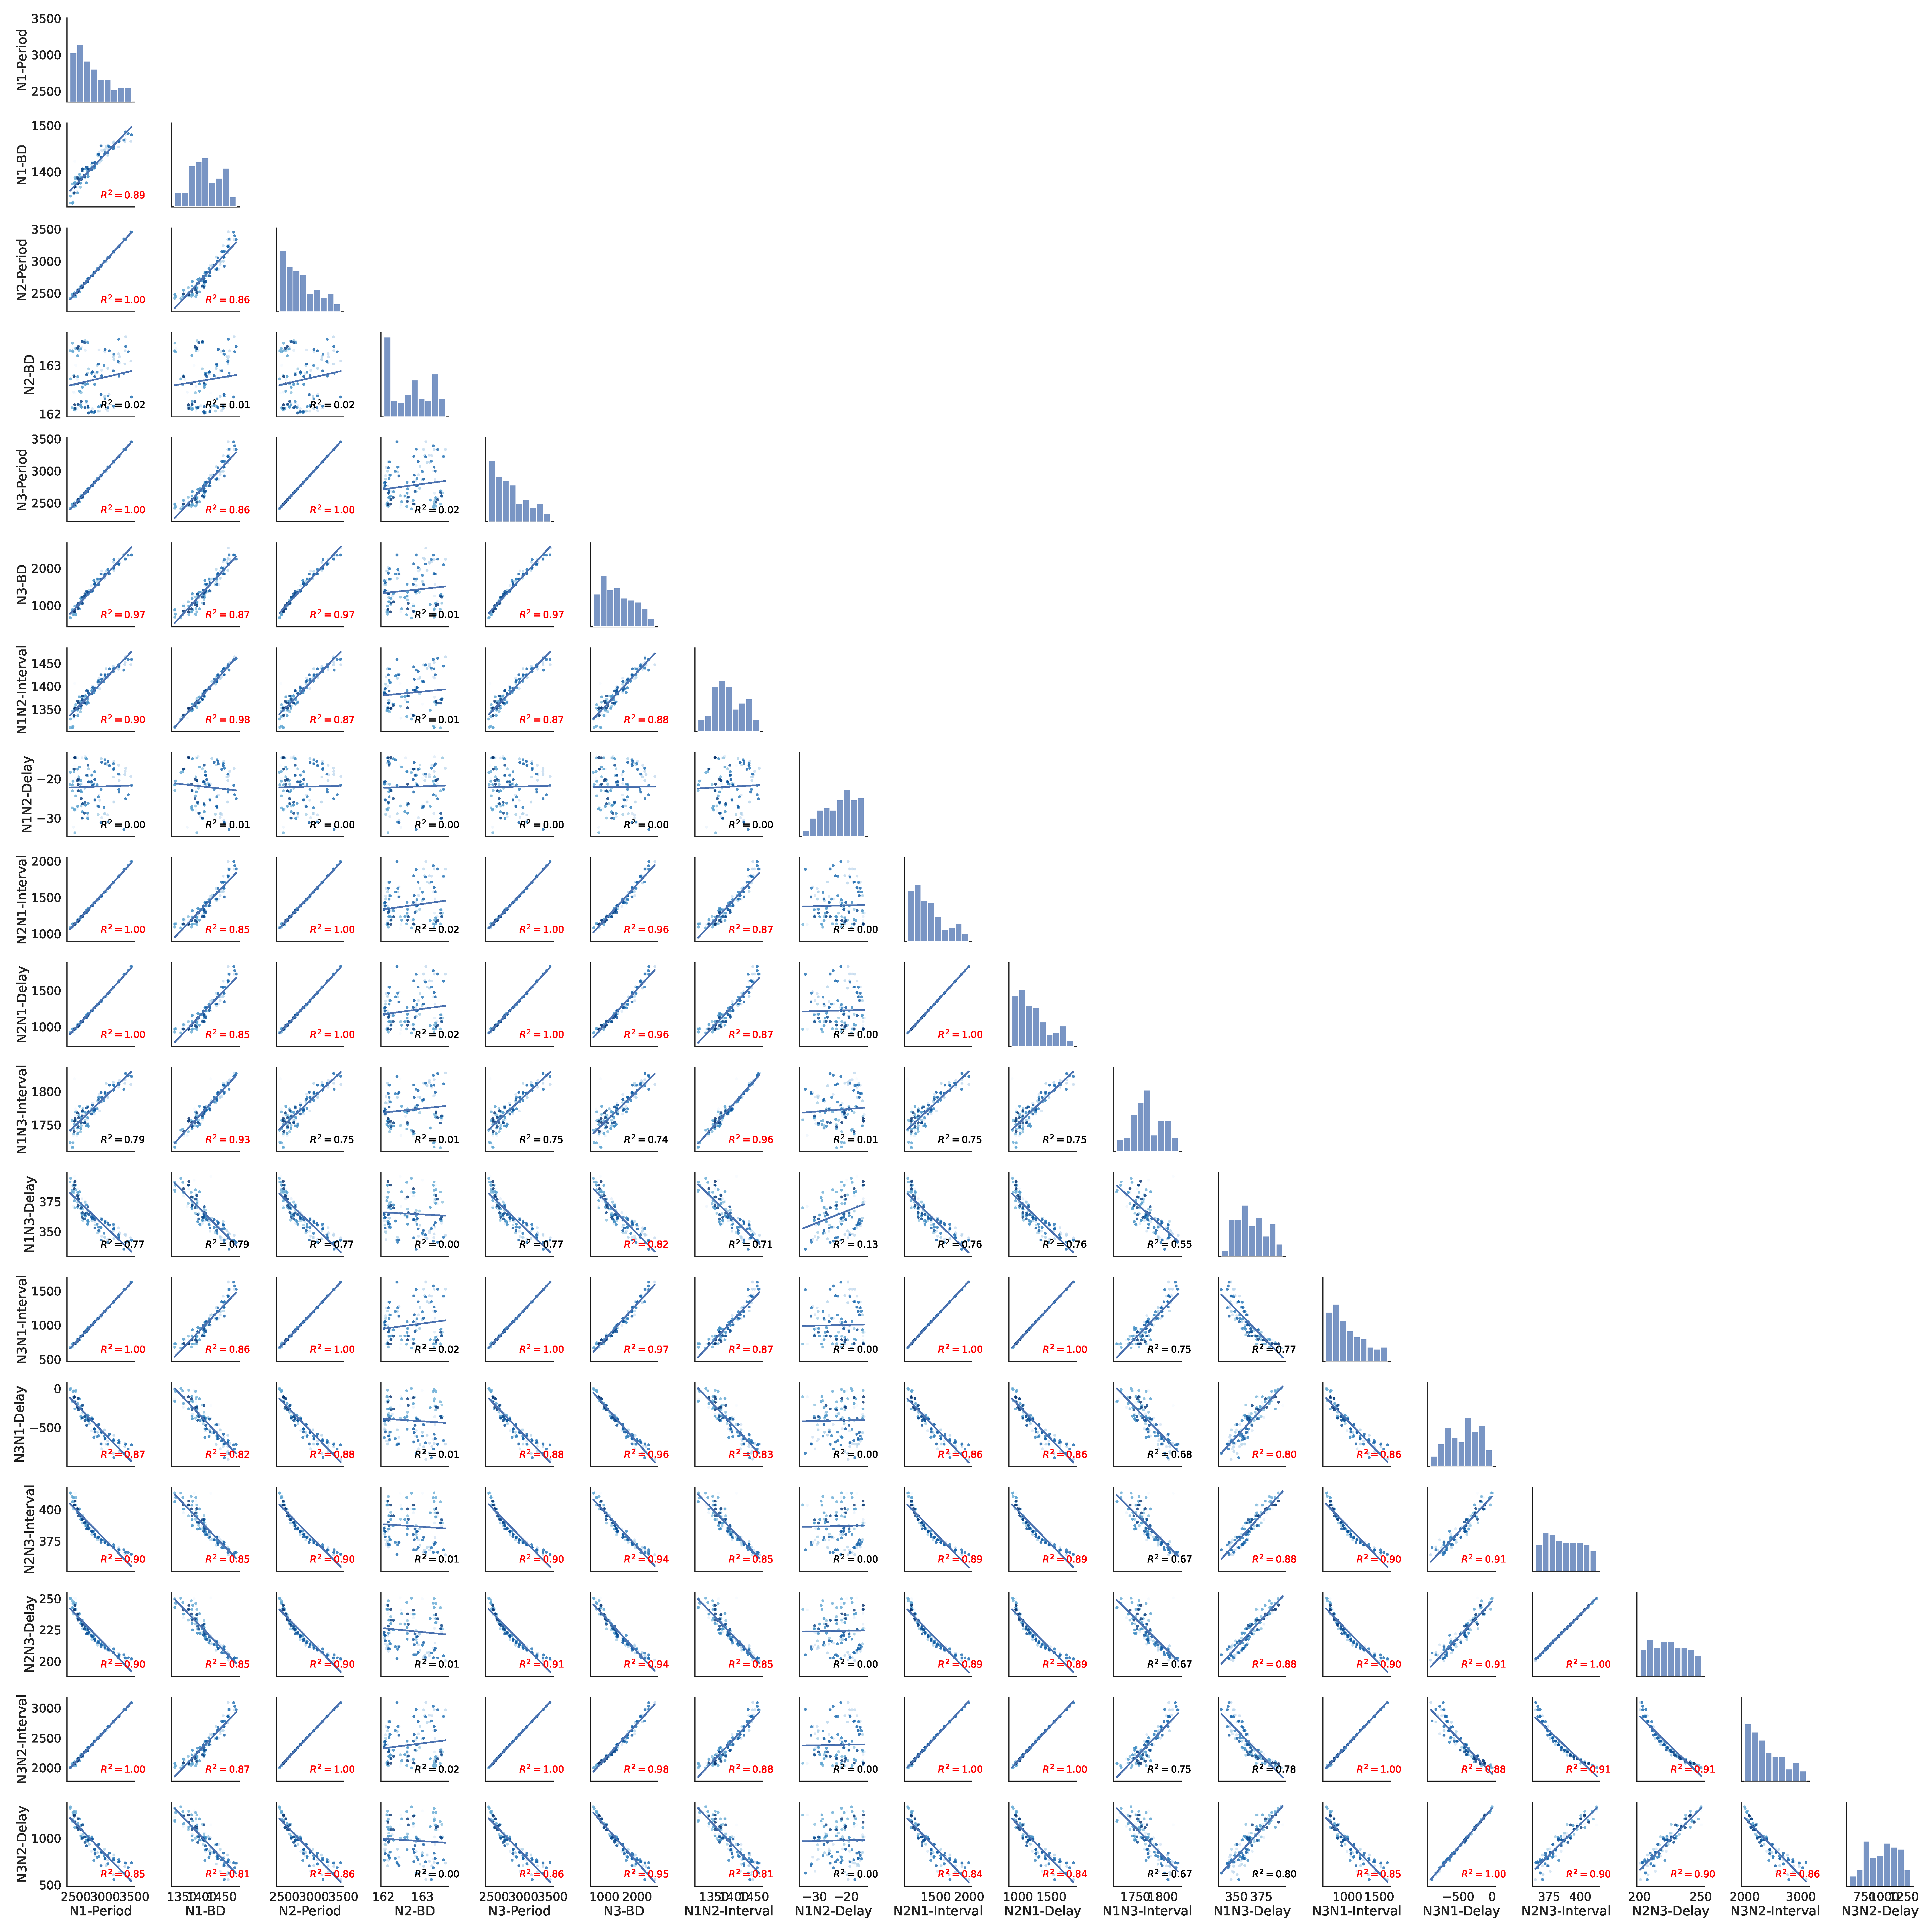
\includegraphics[width=\textwidth]{./invariants/data/MODEL/n3t_driven/images/3phases/output_pairplot.pdf}
	\caption{\textbf{N3t stimulation}: Pairplot with all possible combination between time intervals within a cycle.}
	\label{fig:model n3t stimulation pairplot}
\end{figure}

\begin{figure}[htbp]
	\centering
	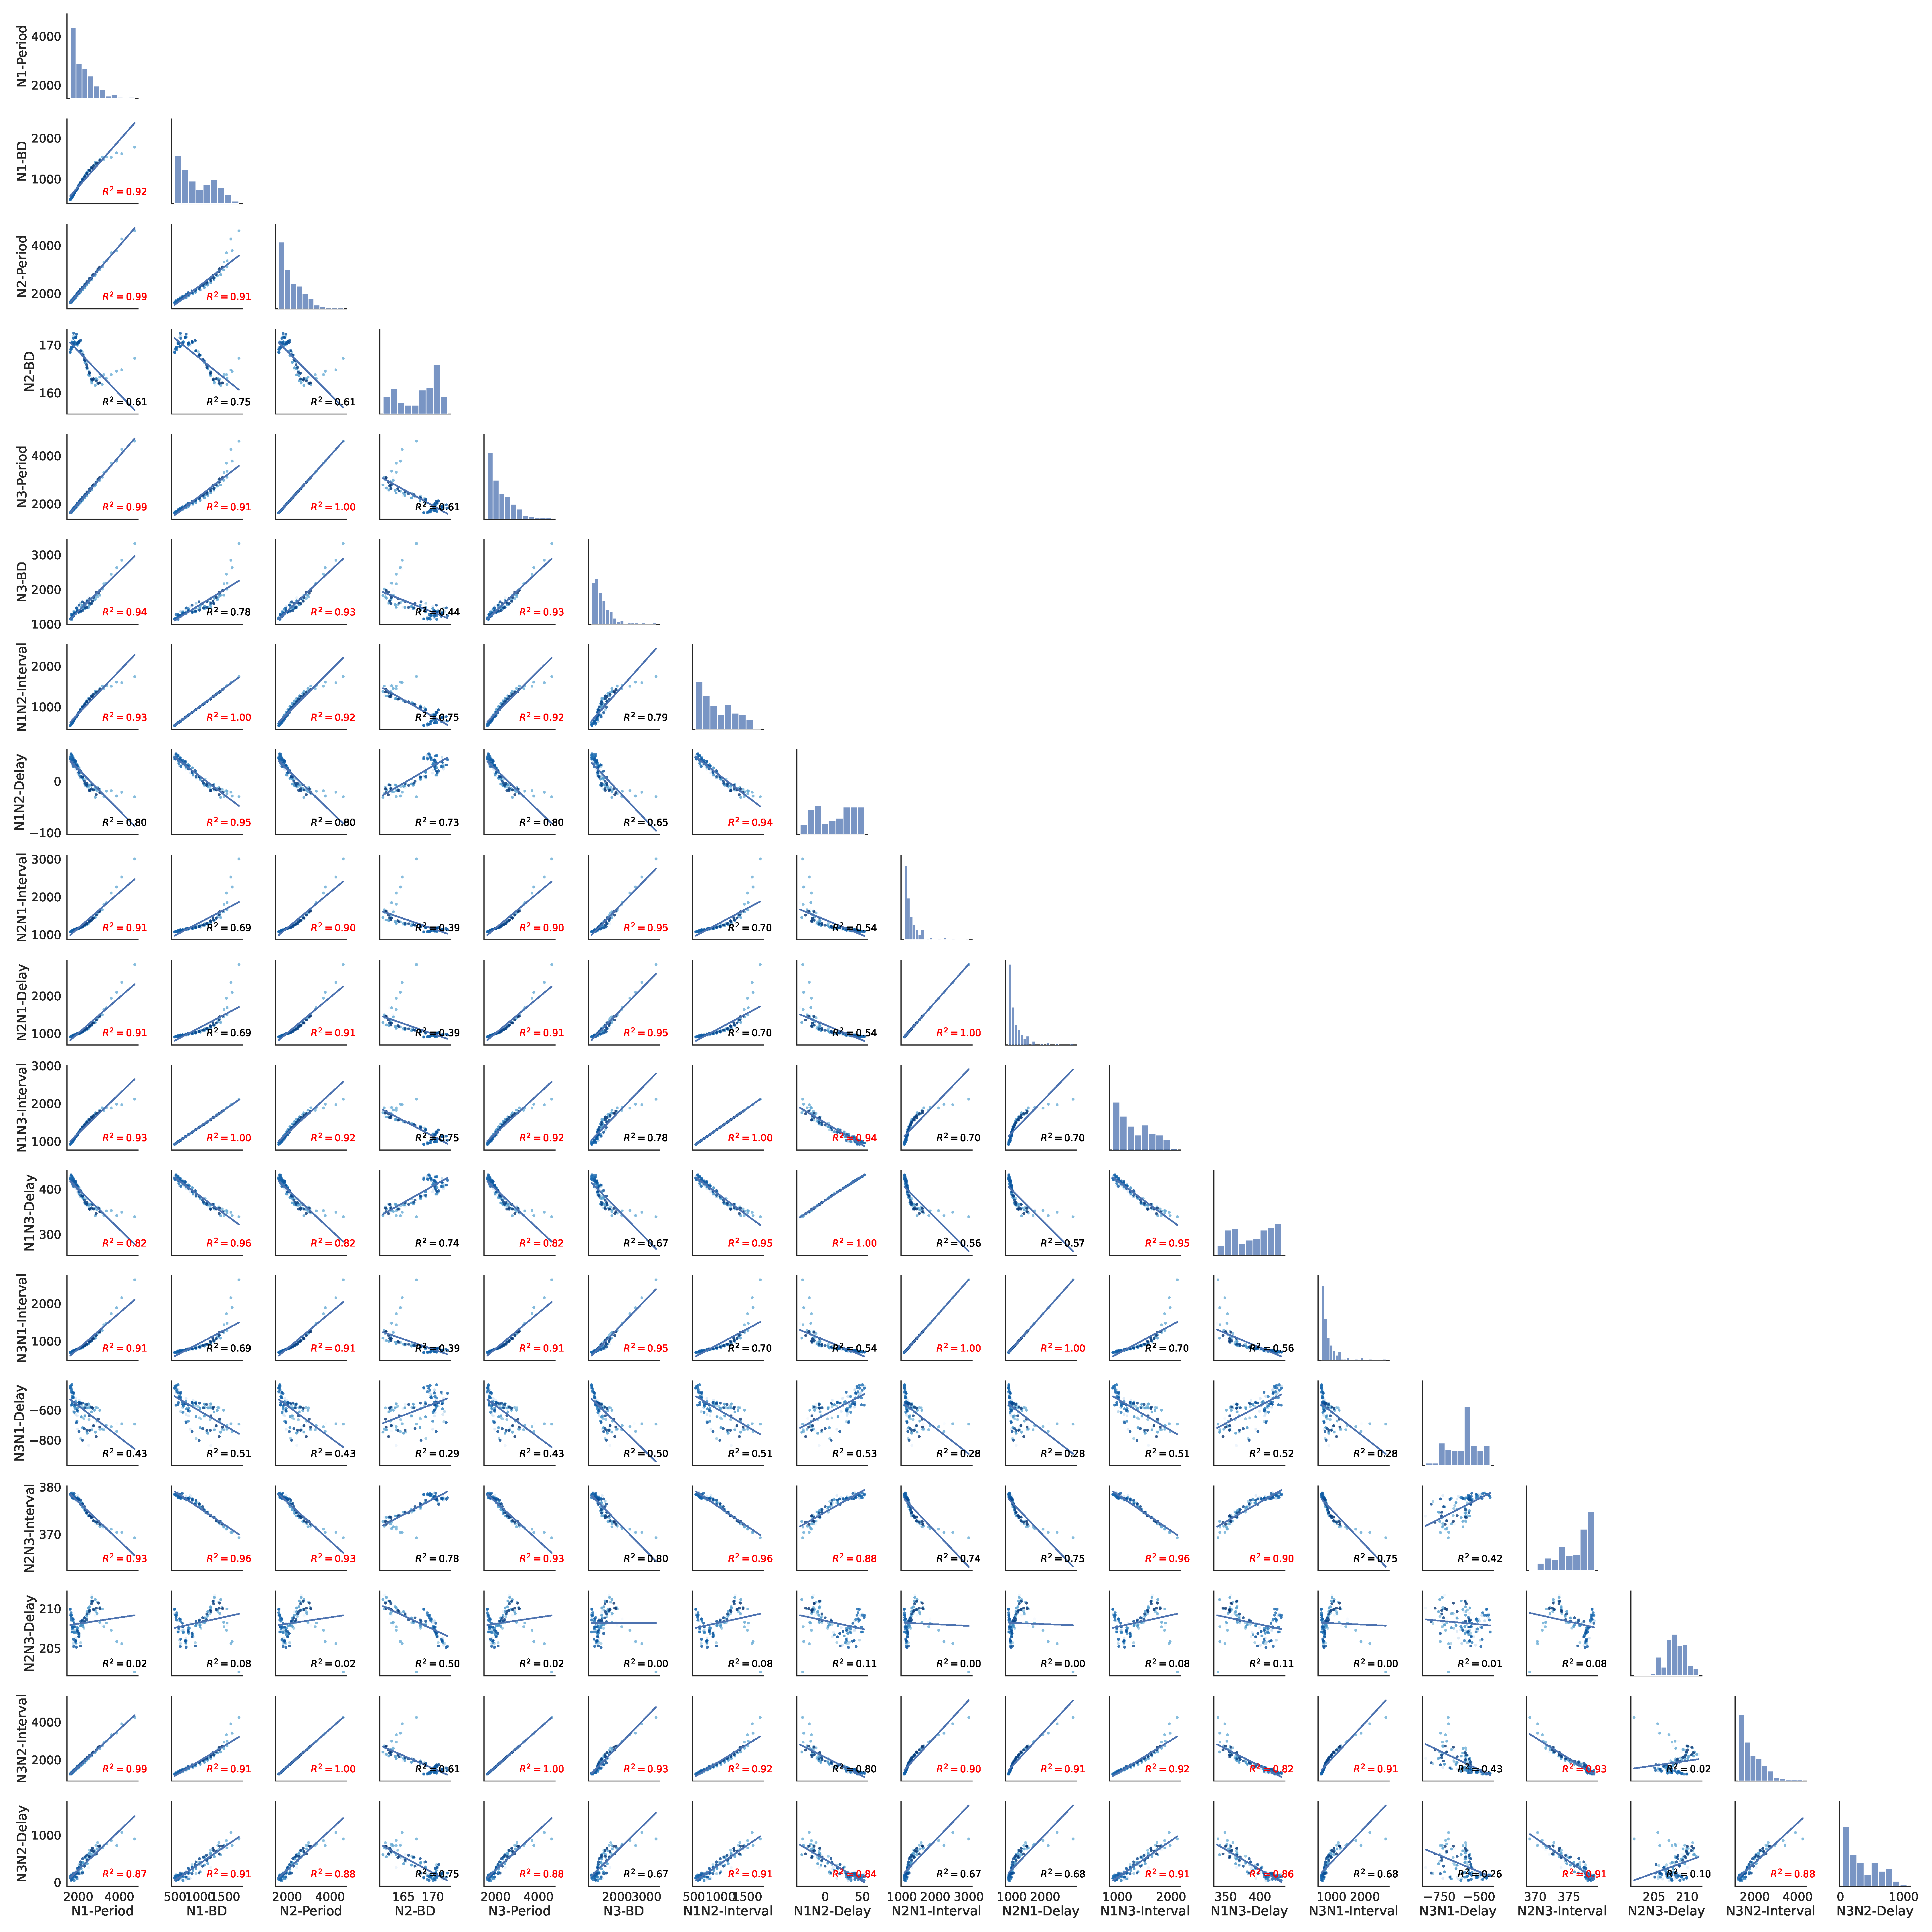
\includegraphics[width=\textwidth]{./invariants/data/MODEL/so_driven/images/3phases/output_pairplot.pdf}
	\caption{\textbf{SO stimulation}: Pairplot with all possible combination between time intervals within a cycle.}
	\label{fig:model so stimulation pairplot}
\end{figure}

%
\subsection{Comparison with two-phase intervals}
During this section we analyzed the sequential dynamical invariants in for three phases, bur we can also define the intervals for two phases of the neurons, taking as reference for example, N1 and N3. This is the case in the work by \cite{elices_robust_2019}, and in the following section we will also use two phases for some of the recordings were the N2 phase was not possible to characterize out of the intracellular recordings. In Figure \ref{fig:invariant n1m model 2 phases} there is a comparison of the linear relations and different intervals conforming the sequence when the references are in N1, N2 and N3 (as we have shown so far) or only for N1 and N3.

When we only consider two phases, we have less possible combinations and the time-intervals that would correspond to the third neuron are contained in the resulting ones. For example as we can see in Fig. \ref{fig:invariant n1m model 2 phases}a), N2N3 delay would be represented by N1N3 delay; N2 burst duration is included in the N2N3 interval. So when analyzing dynamical invariants in two-phase intervals each interval is more informative of the variability constrains cycle-by-cycle. 

\begin{figure}[hbt!]
	\begin{minipage}[b]{0.9\textwidth}
		\raggedleft
		\begin{minipage}[b]{0.53\textwidth}
			\raggedleft
			\begin{overpic}[width=\textwidth]{methods-paper-modelo/Intervals_figure_complete.png}
				\put(0,40){\large\textbf{a)}}
			\end{overpic}
%			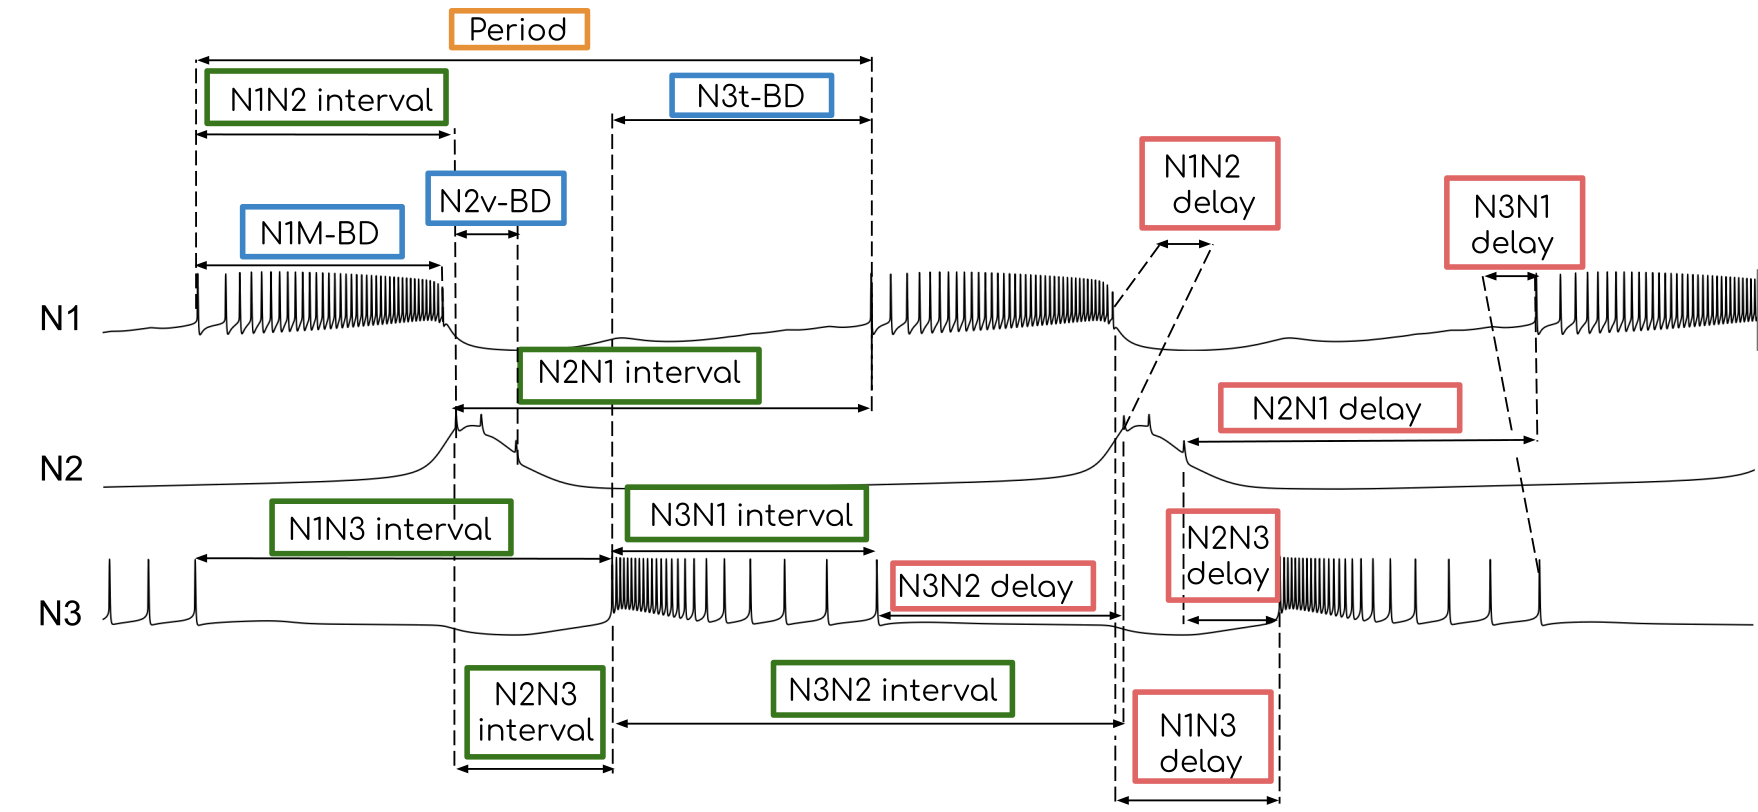
\includegraphics[width=\textwidth]{methods-paper-modelo/Intervals_figure_complete.png}
		\end{minipage}
		\centering 
		\begin{minipage}[b]{0.3\textwidth}
			\centering
			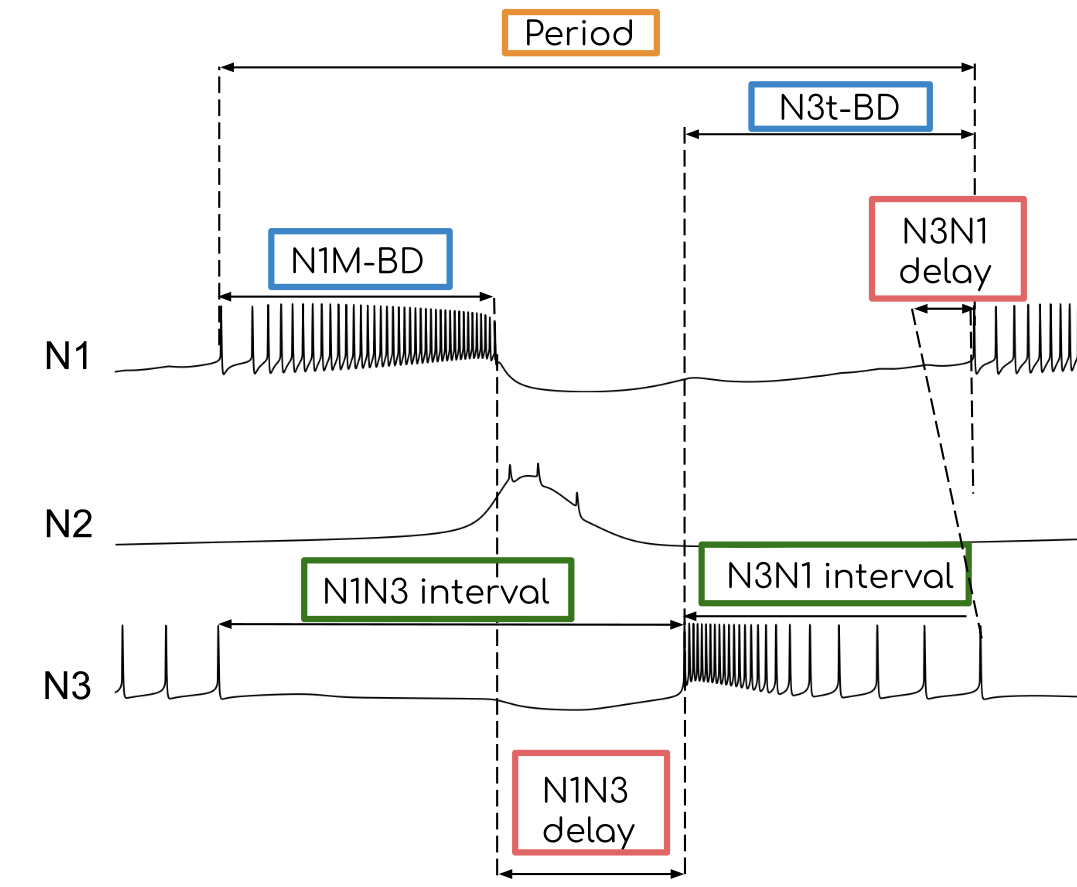
\includegraphics[width=\textwidth]{methods-paper-modelo/Intervals_figure_complete_2_phases.png}
		\end{minipage}	
	\end{minipage}\\
	\begin{minipage}[b]{0.53\textwidth}
		\centering
		\begin{minipage}[b]{\textwidth}
			\centering
			\begin{overpic}[width=\textwidth]{invariants/data/MODEL/n1m_driven/images/3phases/_durations.pdf}
				\put(0,35){\large\textbf{b)}}
			\end{overpic}
		\end{minipage}\
		\begin{minipage}[b]{\textwidth}
			\centering
			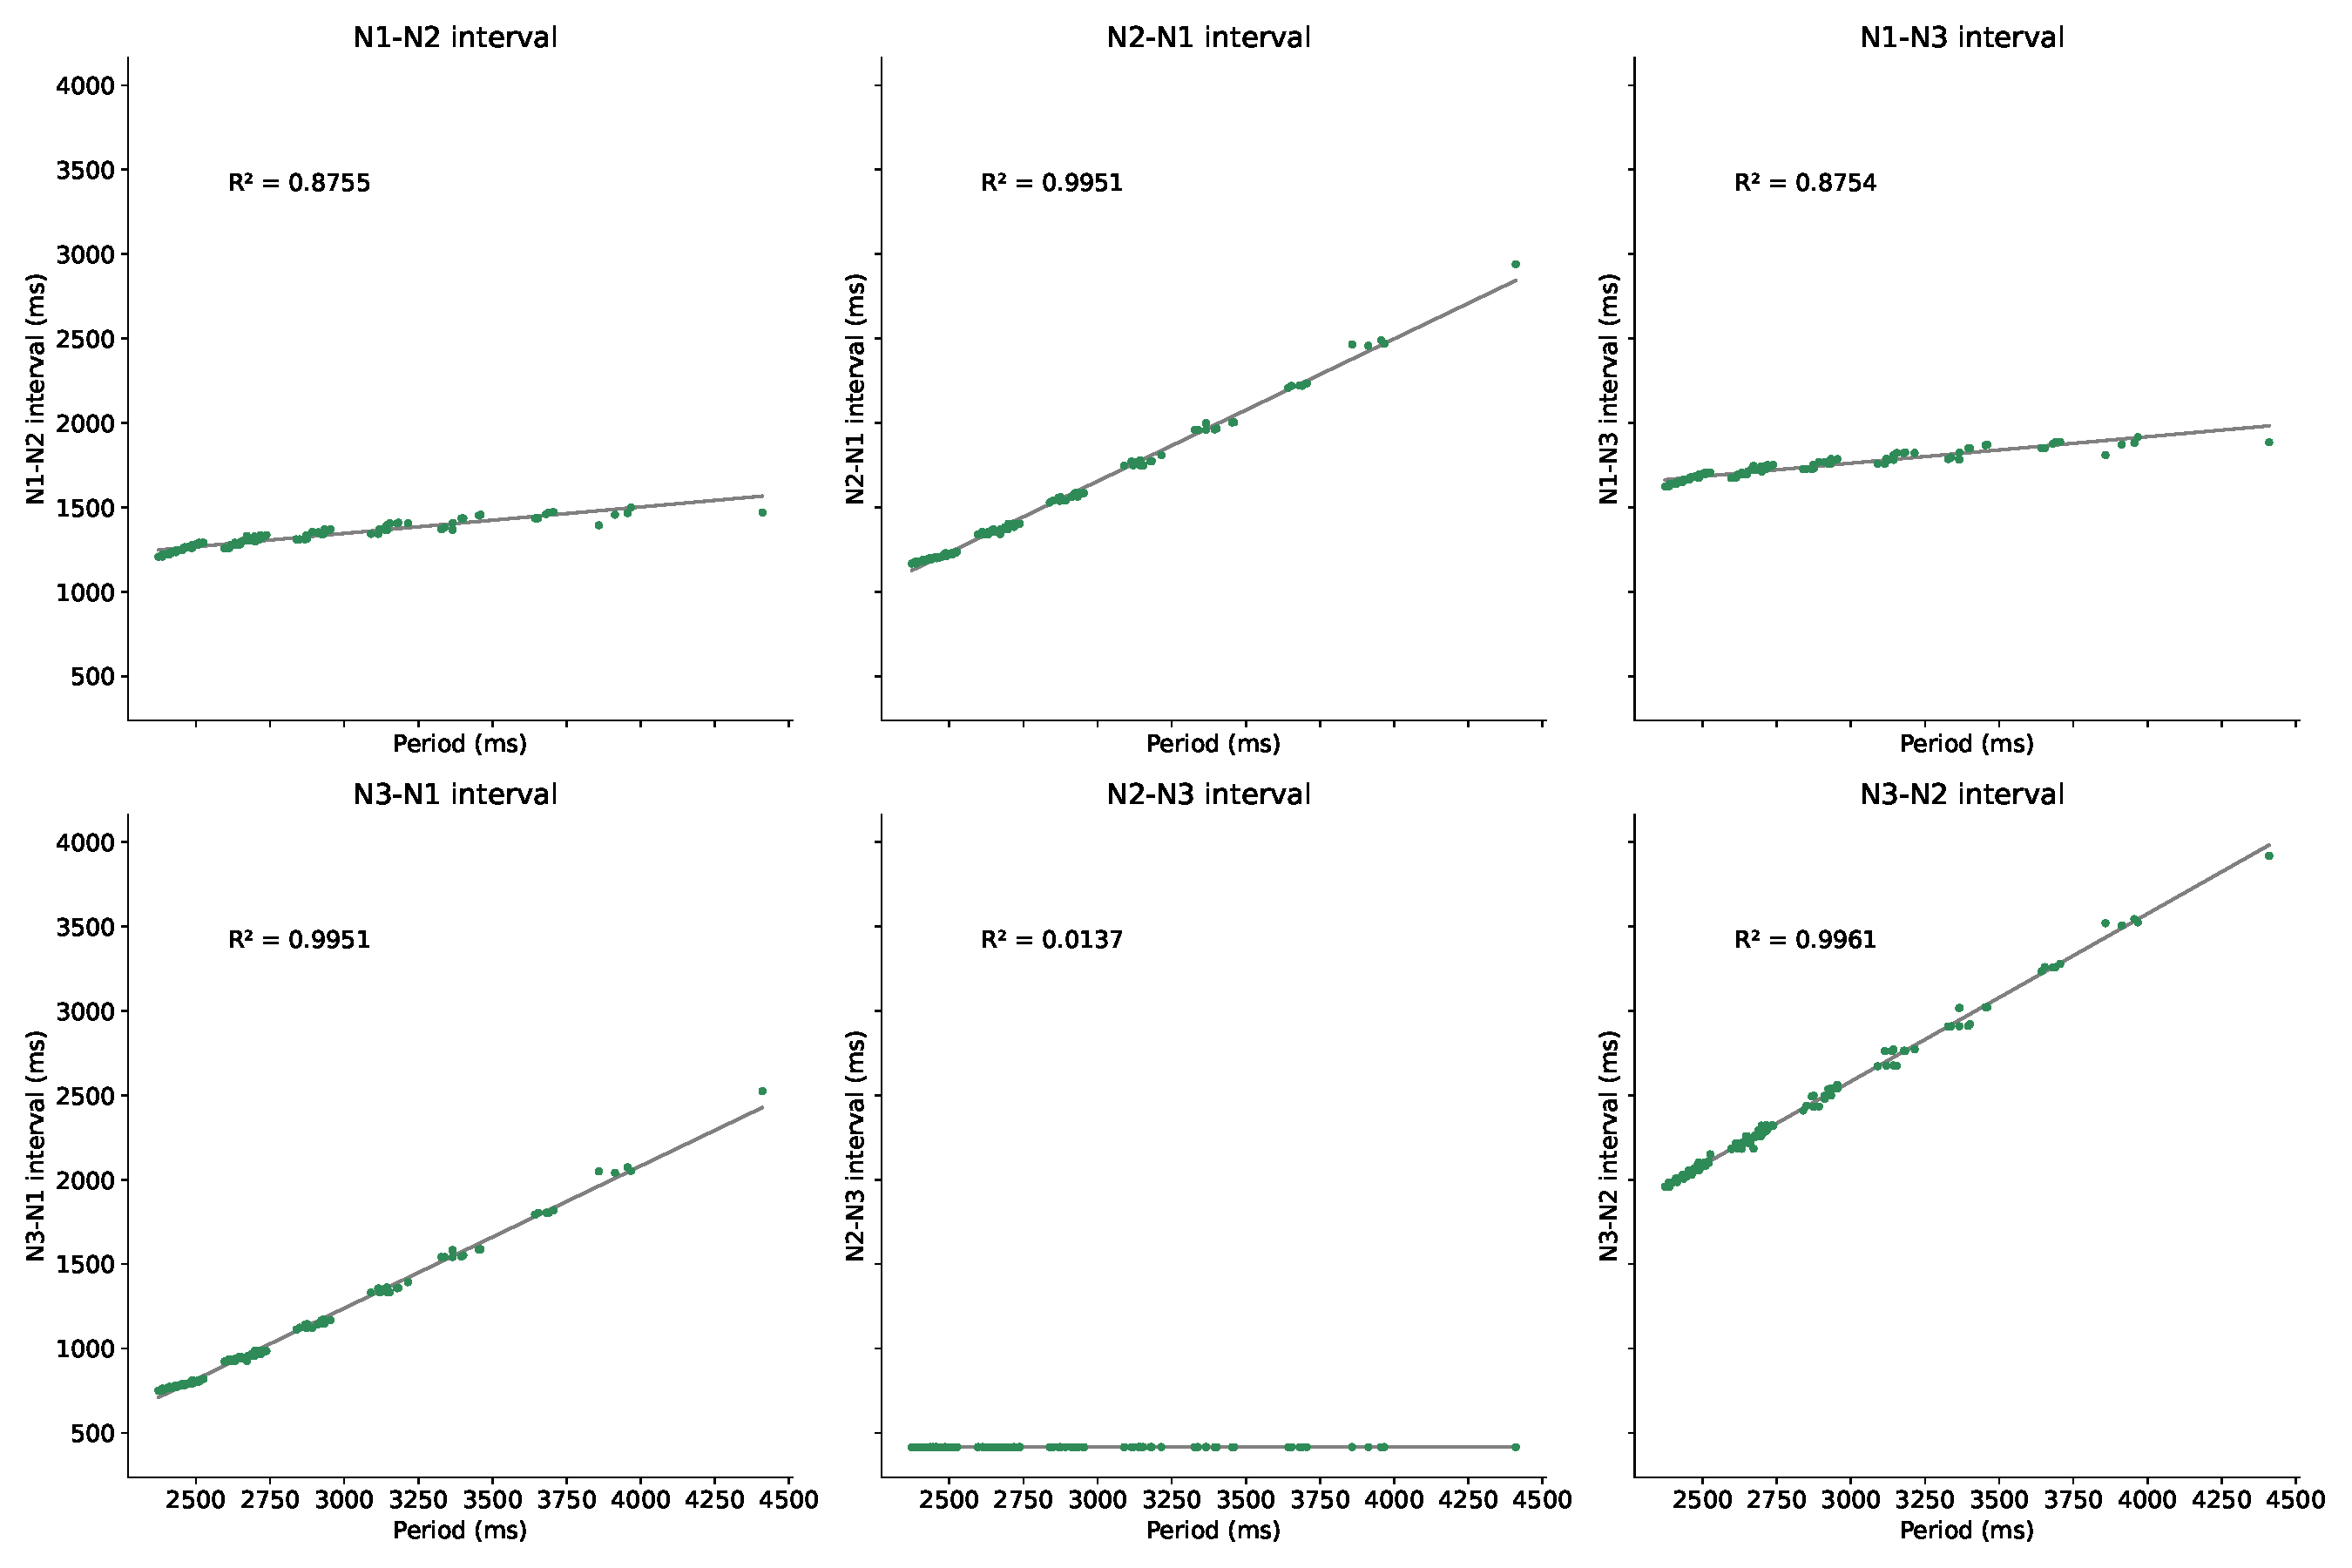
\includegraphics[width=\textwidth]{invariants/data/MODEL/n1m_driven/images/3phases/_intervals.pdf}
		\end{minipage}\
		\begin{minipage}[b]{\textwidth}
			\centering
			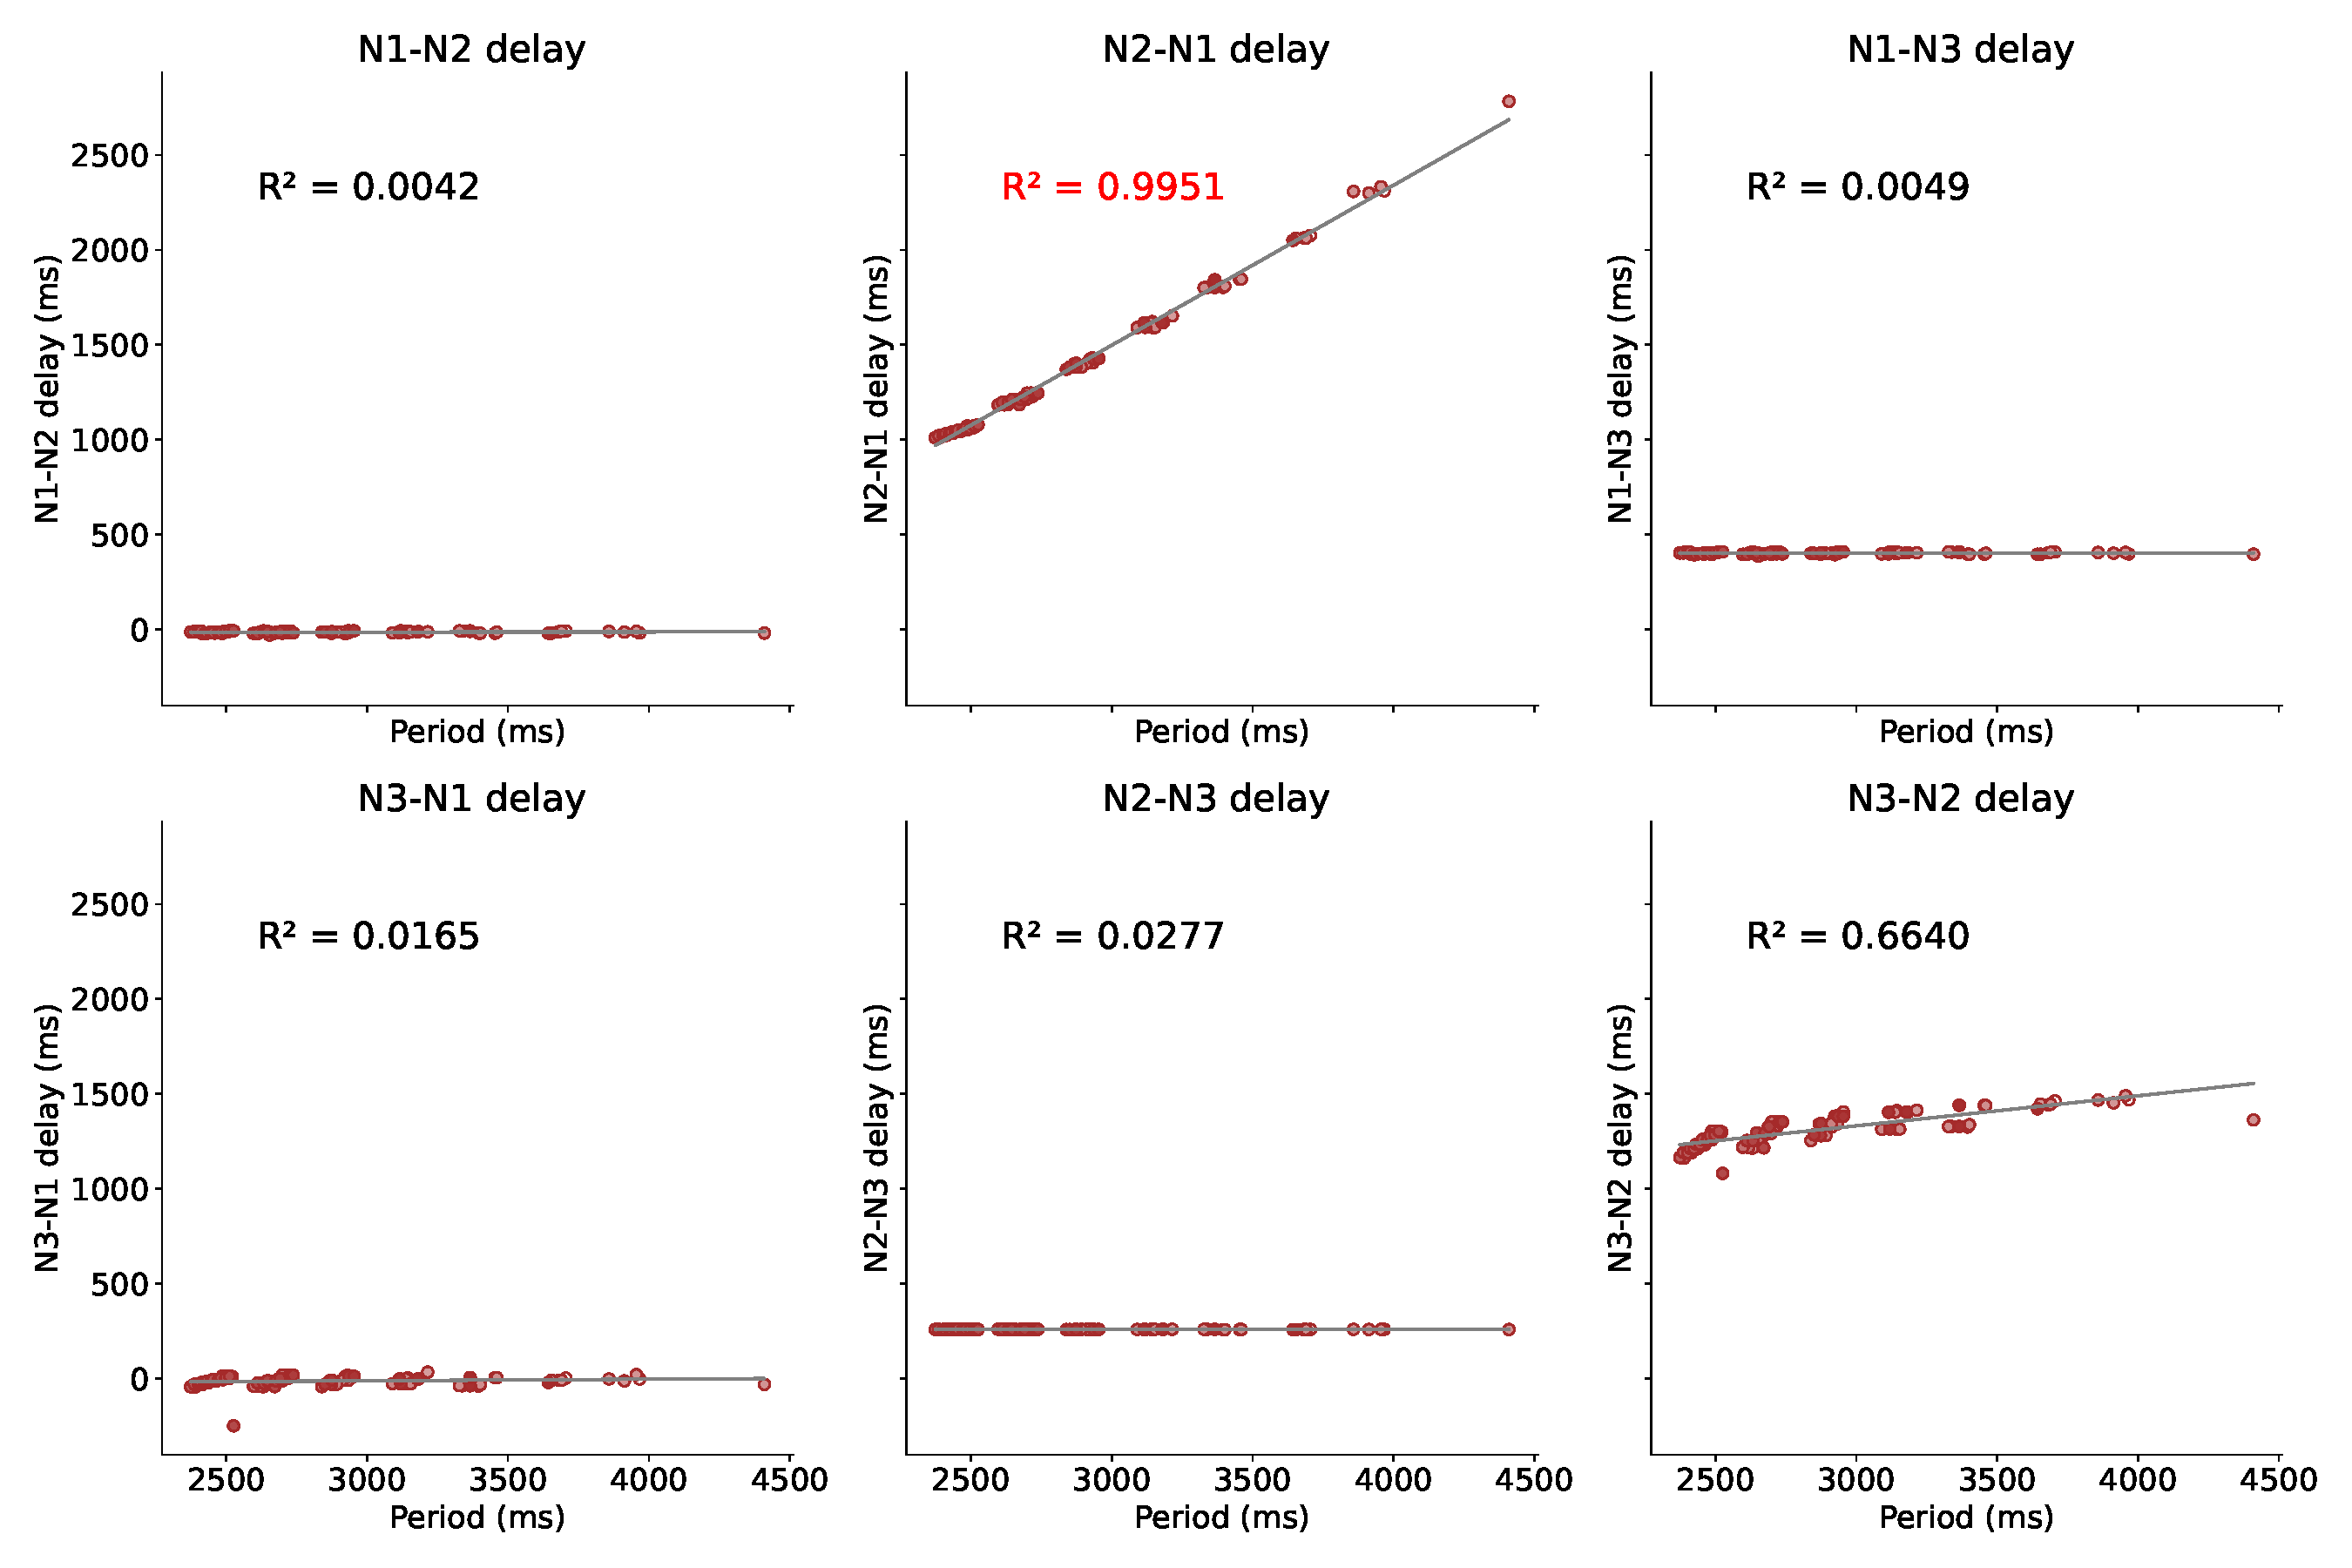
\includegraphics[width=\textwidth]{invariants/data/MODEL/n1m_driven/images/3phases/_delays.pdf}
		\end{minipage}
	\end{minipage}
	\begin{minipage}[b]{0.45\textwidth}
		\centering
		\begin{minipage}[b]{\textwidth}
			\centering
			\begin{overpic}[width=\textwidth]{invariants/data/MODEL/n1m_driven/images/2phases/_durations.pdf}
				\put(0,50){\large\textbf{c)}}
		\end{overpic}
		\end{minipage}\
		\begin{minipage}[b]{\textwidth}
			\centering
			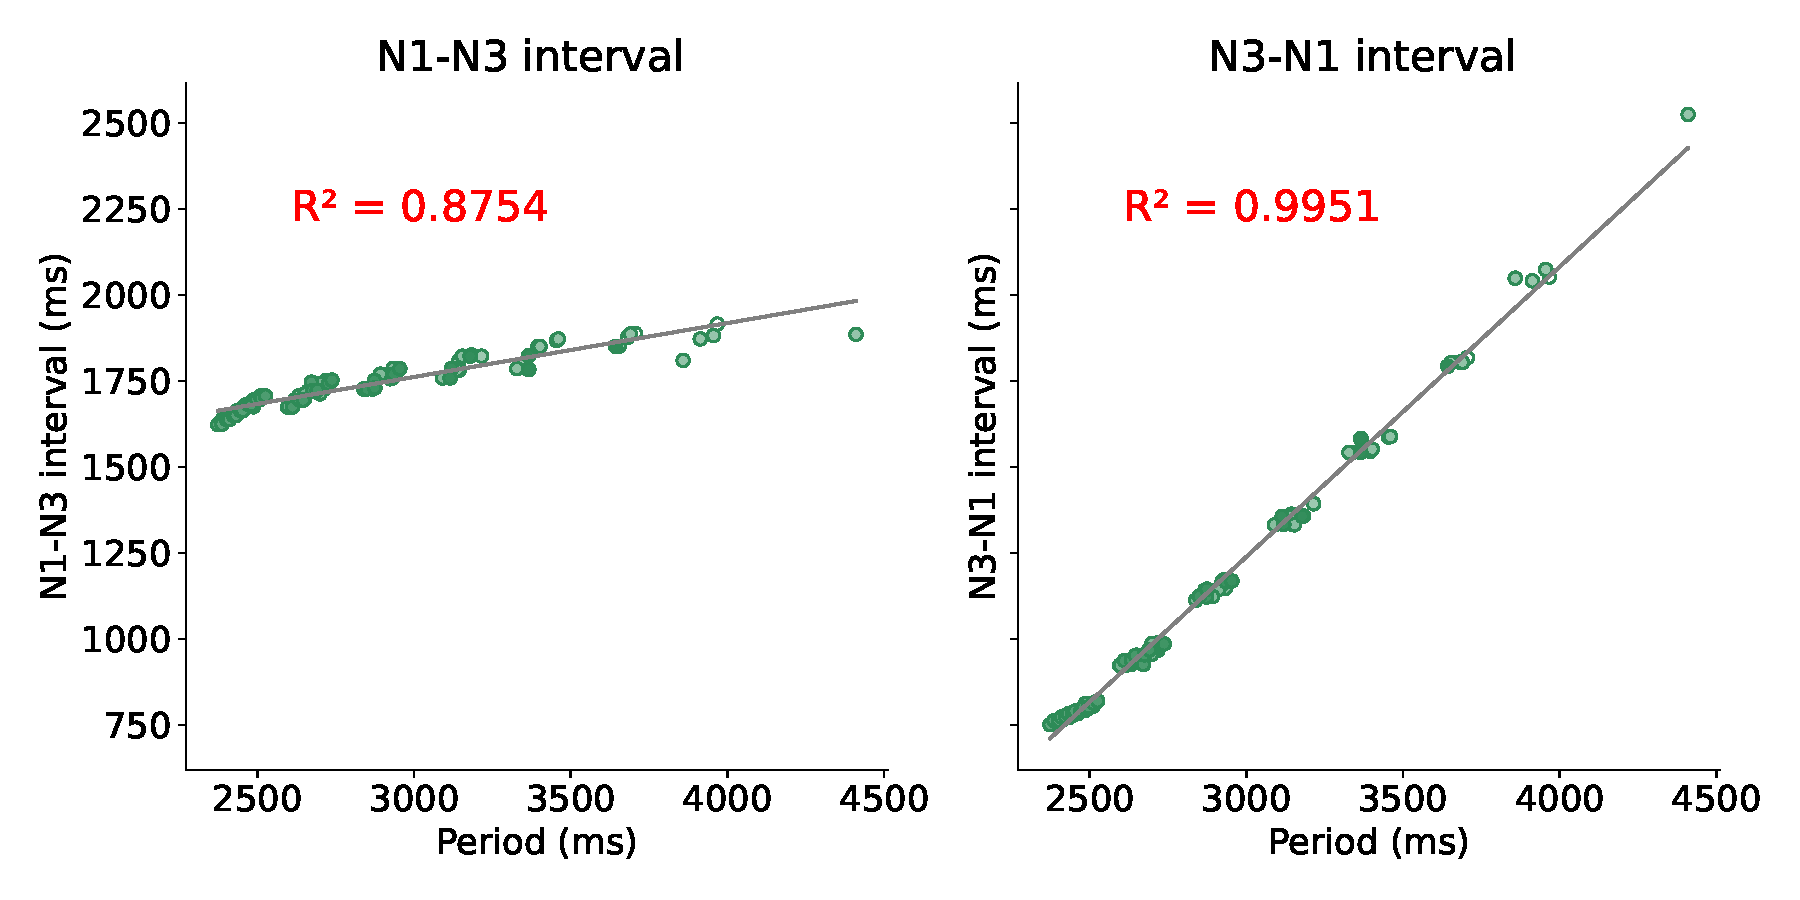
\includegraphics[width=\textwidth]{invariants/data/MODEL/n1m_driven/images/2phases/_intervals.pdf}
		\end{minipage}\
		\begin{minipage}[b]{\textwidth}
			\centering
			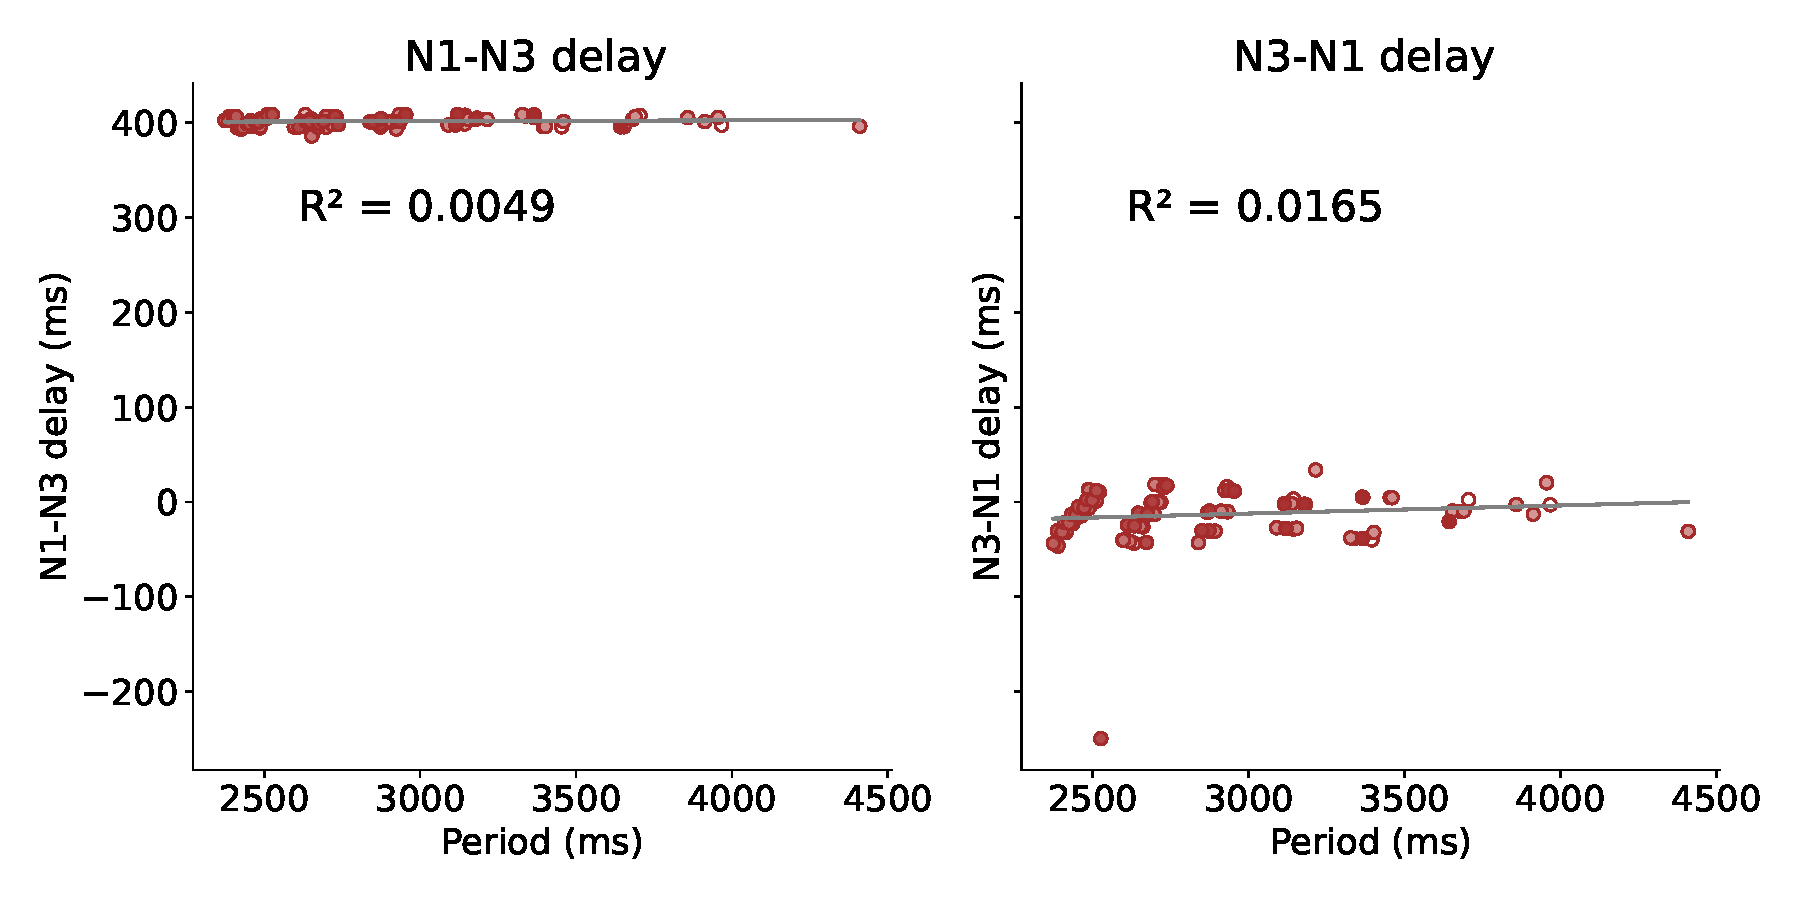
\includegraphics[width=\textwidth]{invariants/data/MODEL/n1m_driven/images/2phases/_delays.pdf}
		\end{minipage}
	
		\vspace{50pt}
	\end{minipage}
	\caption{a) Representation of the intervals for each cycle when considering three or two phases (left and right, respectively). b) Interval correlations to period for SO-driven simulation for 3 phases. First row: Burst duration. Second and third row: Two-neuron intervals. Forth and fifth row: Two-neuron delays (Data shown in Fig. \ref{fig:invariant n1m}). c) Interval correlations to period for N1M-driven simulation for 2 phases. First row: Burst duration. Second row: Two-neuron intervals. Third row: Two-neuron delays. For b) and c) the linear relationships are quantified by the $R^2$ values of the regression.}
	\label{fig:invariant n1m model 2 phases}
\end{figure}


\clearpage
\newpage

\section{Experimental results in \textit{Lymnaea Stagnalis}}
\label{sec:experimental sussex}
When studying temporal structures in neural dynamics, the definition of the time references is a key first point. In the computational analysis in the previous section, the time reference to define the intervals were first and last spike of each burst. In that case, as in the case of interneurons in \textit{C. maenas} the CPG phases are directly related with the bursting activity of these neurons and the burst can be consistently defined by the first and last spike. However, in the case of \textit{Lymnaea stagnalis}, activity is usually characterized using recordings from both interneurons and motoneurons \parencite{elliott_interactions_1985, staras_pattern-generating_1998, benjamin_distributed_2012}. This leads to the need of a combination of burst references to characterize the phases of the CPG based on the time intervals cycle by cycle. Thus, for this analysis, we will consider the three phases in the CPG, protraction, rasp and swallow, that are associated mainly to N1M, N2v and N3t neurons. Since it is not always possible to record those neurons at the same time (specially N2v that is in the ventral side), we will define them by a combination of interneurons and motoneurons following their activity at each phase. For example, in Figure \ref{fig:example lymnaea phases recording} the three phases in the  CPG are marked by a colored background over the recording, note how it can be delimited by the neurons in the circuit but some of the motoneurons cover several phases, as it is the case of B4 in panel a) or B3 in panel b). Also phases can be defined by the first and last spike, as it is the case for phase N3 and neuron B8, but in other cases as the phase N2, the reference is the hyperpolarization of some neurons, such as the strong inhibition visible in neuron B5 in panel b). Also, depolarization of some neurons carry relevant information, since for example in the case of B1 the "bumps" visible represent the N1 phase, by the connection between N1M and B1. Therefore, to characterize the time sequences in the feeding CPG, we need compound reference from several neural recordings that can be summarized as in Table \ref{table:cpg ref intervals}. Note that, although different time references must be taken into account when reaching conclusions about the time-interval restrictions and analysis, all possible intervals conforming each cycle between the neurons are taking into account in this analysis (see \ref{subsec:intervals}), so the restrictions and analysis are still relevant.

\begin{table}[htb!]
	\centering
	\begin{tabular}{cl|l|l}
		\multicolumn{1}{l}{}                                 & \multicolumn{1}{c|}{\textbf{N1-Protraction}} & \multicolumn{1}{c|}{\textbf{N2-Rasp}} & \multicolumn{1}{c}{\textbf{N3-Swallow}} \\ \hline
		\multicolumn{1}{c|}{\multirow{3}{*}{\textbf{Start}}} & Last spike of N3t/B3                         & Inhibition of B5                      & First spike of B8                       \\
		\multicolumn{1}{c|}{}                                & Depolarization or first spike in B1          &                                       &                                         \\
		\multicolumn{1}{c|}{}                                & First spike in B6                            &                                       &                                         \\ \hline
		\multicolumn{1}{c|}{\multirow{2}{*}{\textbf{End}}}   & Last spike of B5                             & First spike of B8                     & Last spike of N3t/B3                    \\
		\multicolumn{1}{c|}{}                                & Hyperpolarization in B1 or B6                &                                       &                                        
	\end{tabular}
	\caption{Time reference boundaries for the three phases in the feeding CPG}
	\label{table:cpg ref intervals}
\end{table}



\begin{figure}[bth!]
	\centering
	\begin{minipage}[b]{\textwidth}
		\makebox[0pt][l]{\hspace*{-130pt}\text{a)}}\\
		\centering
		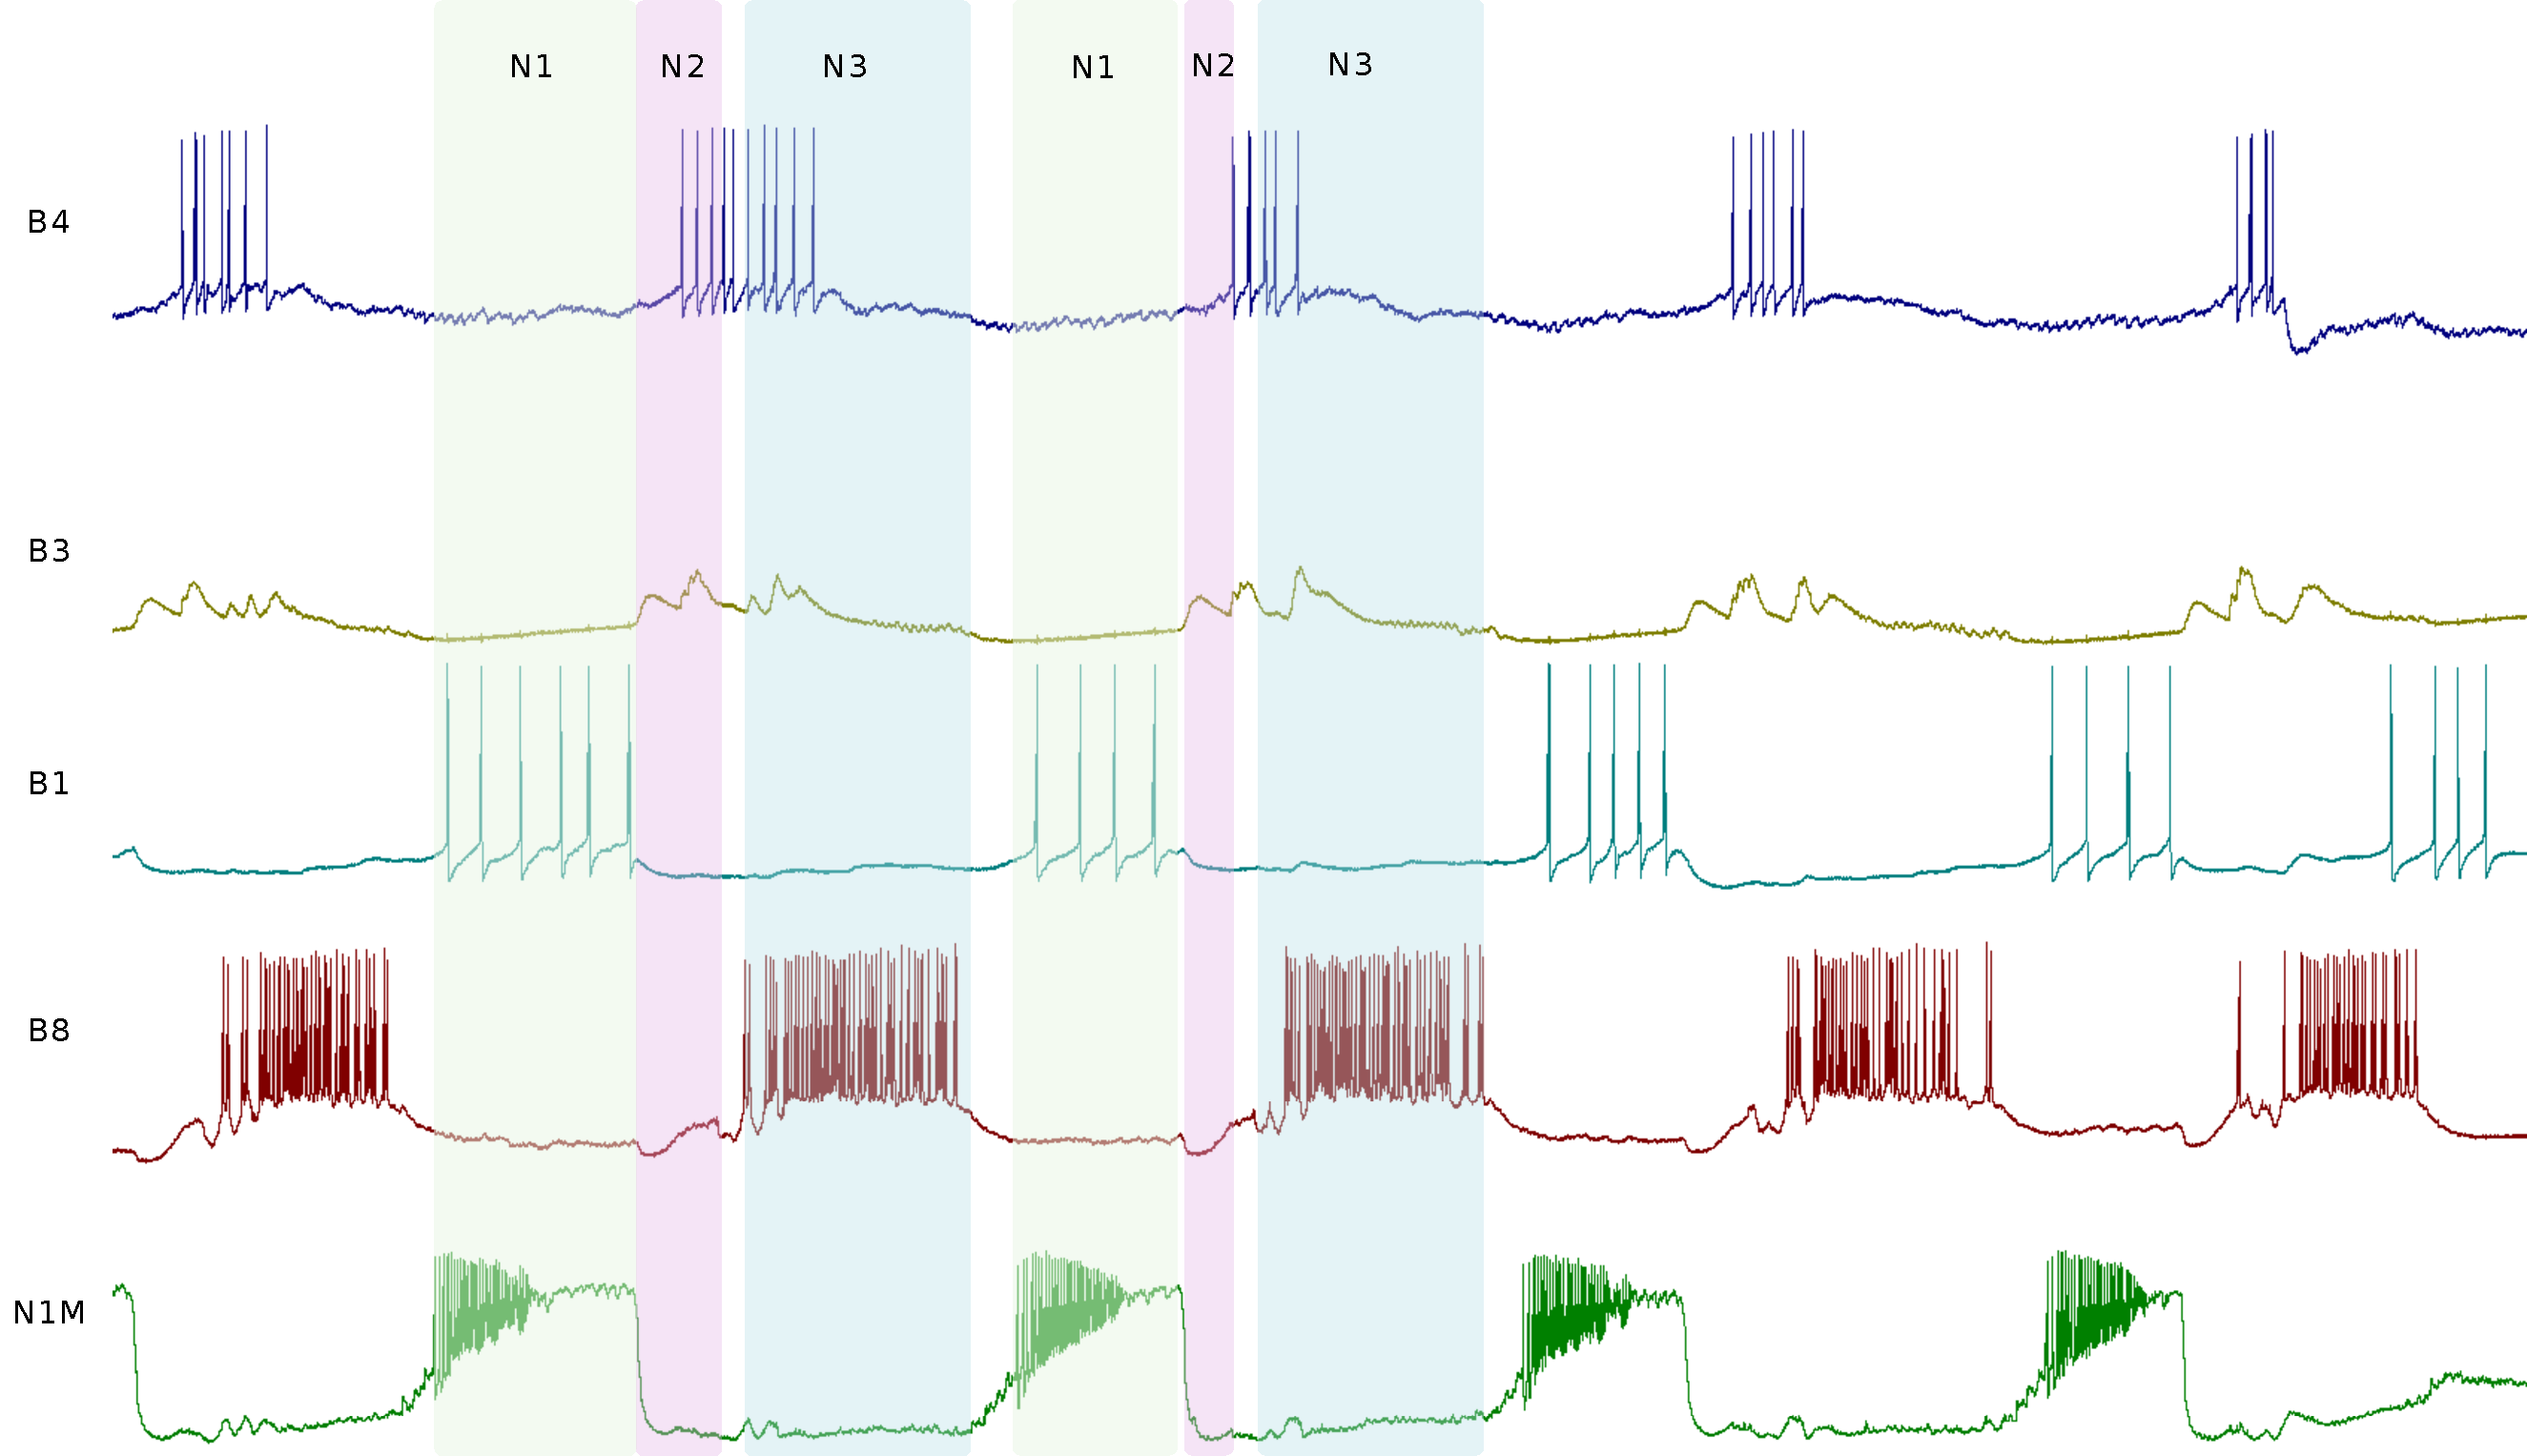
\includegraphics[width=0.9\textwidth]{img/invariants/example_phases_1.pdf}
	\end{minipage}
	\vspace{20pt}
	\begin{minipage}[b]{\textwidth}
		\makebox[0pt][l]{\hspace*{-130pt}\text{b)}}\\
		\centering
		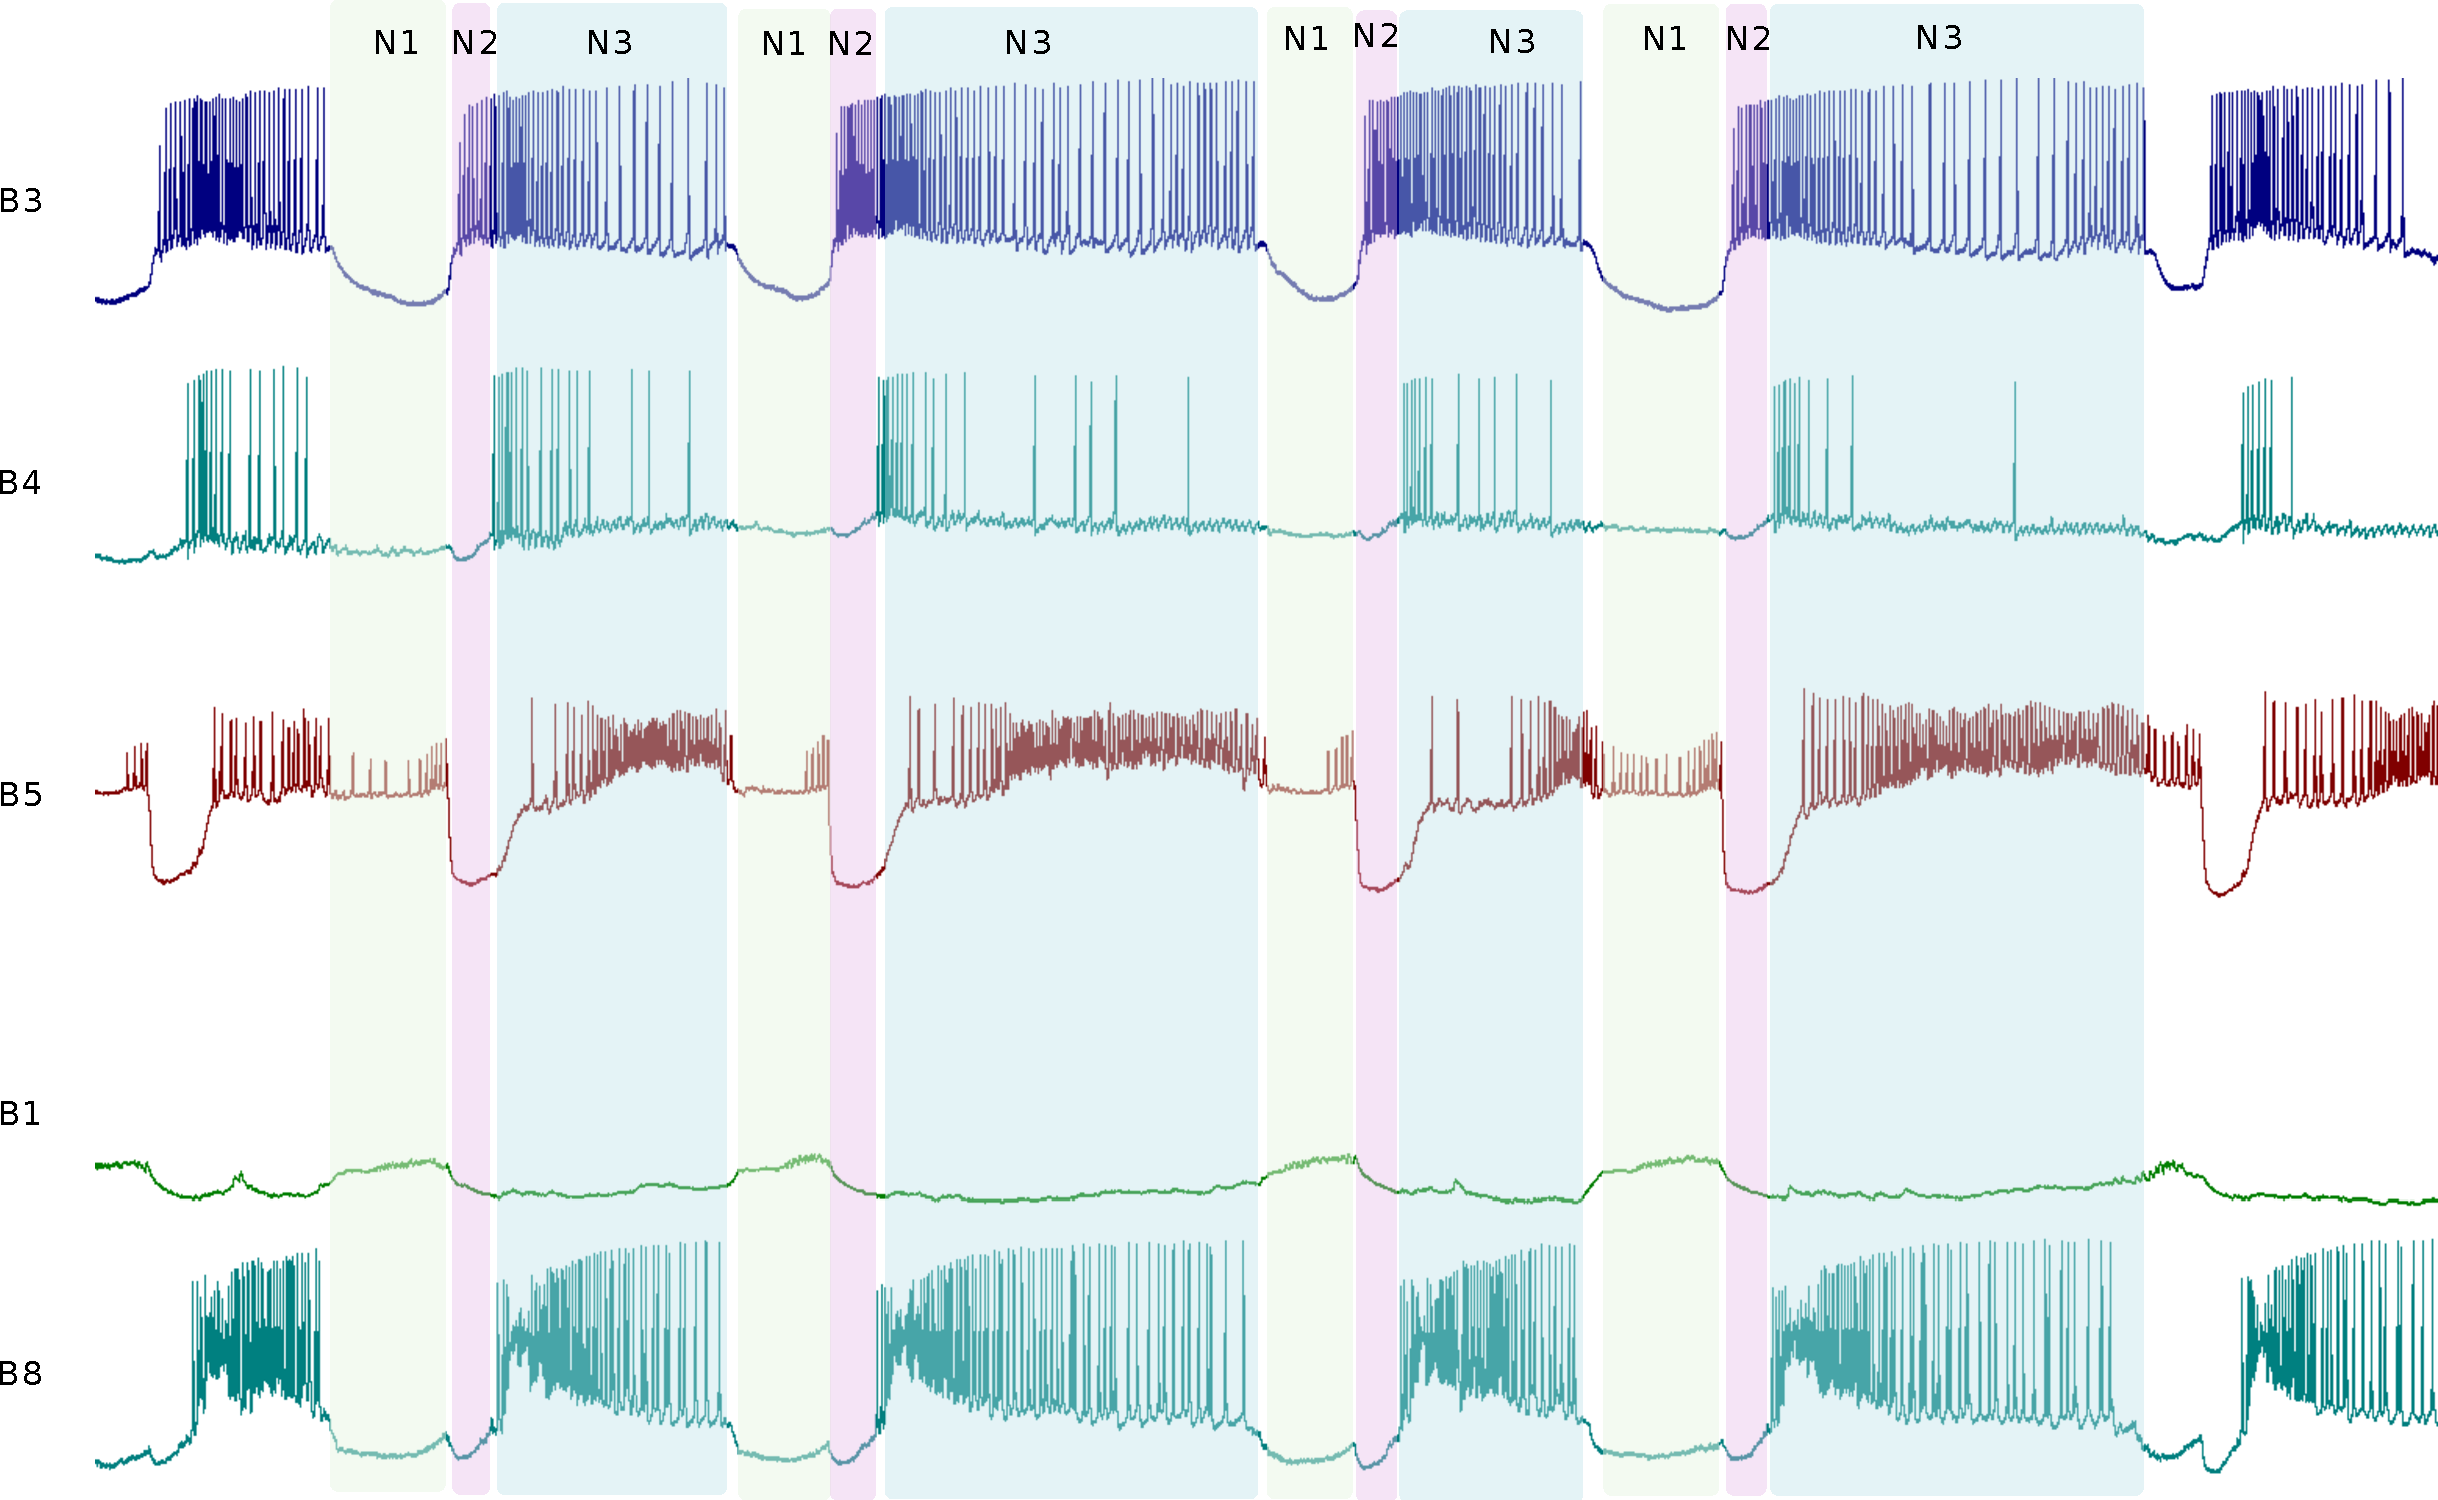
\includegraphics[width=0.9\textwidth]{img/invariants/example_phases_2.pdf}
	\end{minipage}
	\caption{Delimitation of phases in the feeding CPG of \textit{Lymnaea stagnalis} based on different recordings. Panel a) intracellular recordings for motoneurons B4,B3,B1 and B8 and the interneuron N1M. Phases are delimited by N1M and B1, that have the same activation time for phase N1, the inhibition of N1M and the start of the depolarization in B8 for phase N2 and the first and last spike of burst B8 for phase N3. Panel b) intracellular recordings for motoneurons B3,B4,B5, B1 and B8. Phases are delimited by B1 depolarization for phase N1, the strong inhibition of B5 for phase N2 and the fisrt and last spike of burst B8 for phase N3.}
	\label{fig:example lymnaea phases recording}
\end{figure}

Another key point in the study of the feeding CPG of \textit{L. stagnalis} is that the generation of the rhythm is a combined action of different cells \cite{benjamin_distributed_2012}, not only interneurons but also motoneurons have a role in the activation \parencite{staras_pattern-generating_1998} and modulatory neurons in the buccal and cerebral ganglia are involved in the rhythm. All these factors affect the rhythm and thus the neuronal sequential activation and how variability is distributed among the different intervals cycle by cycle. Also, not all the neurons are involved every time the rhythm is active, and that gives also information about the different contexts in which the rhythm is taking part. For example, the rhythm can be activated by the presence of food or sucrose stimulation, in which case the animal needs to initiate the activity and ingest food, the rhythm is started by the stimulation of the lip nerve that also stimulates N1M. Also, even at the absence of food but when the animal is hungry, the CPG can be activated, in this case with a strong role of N3t as modulator. The modulation of the rhythm is also a key aspect and modulatory neurons as SO or CV1a control the rhythm after its initiation, showed to have distinct alternative roles in the activity \parencite{kemenes_multiple_2001}. 

\begin{figure}[bth!]
	\centering
	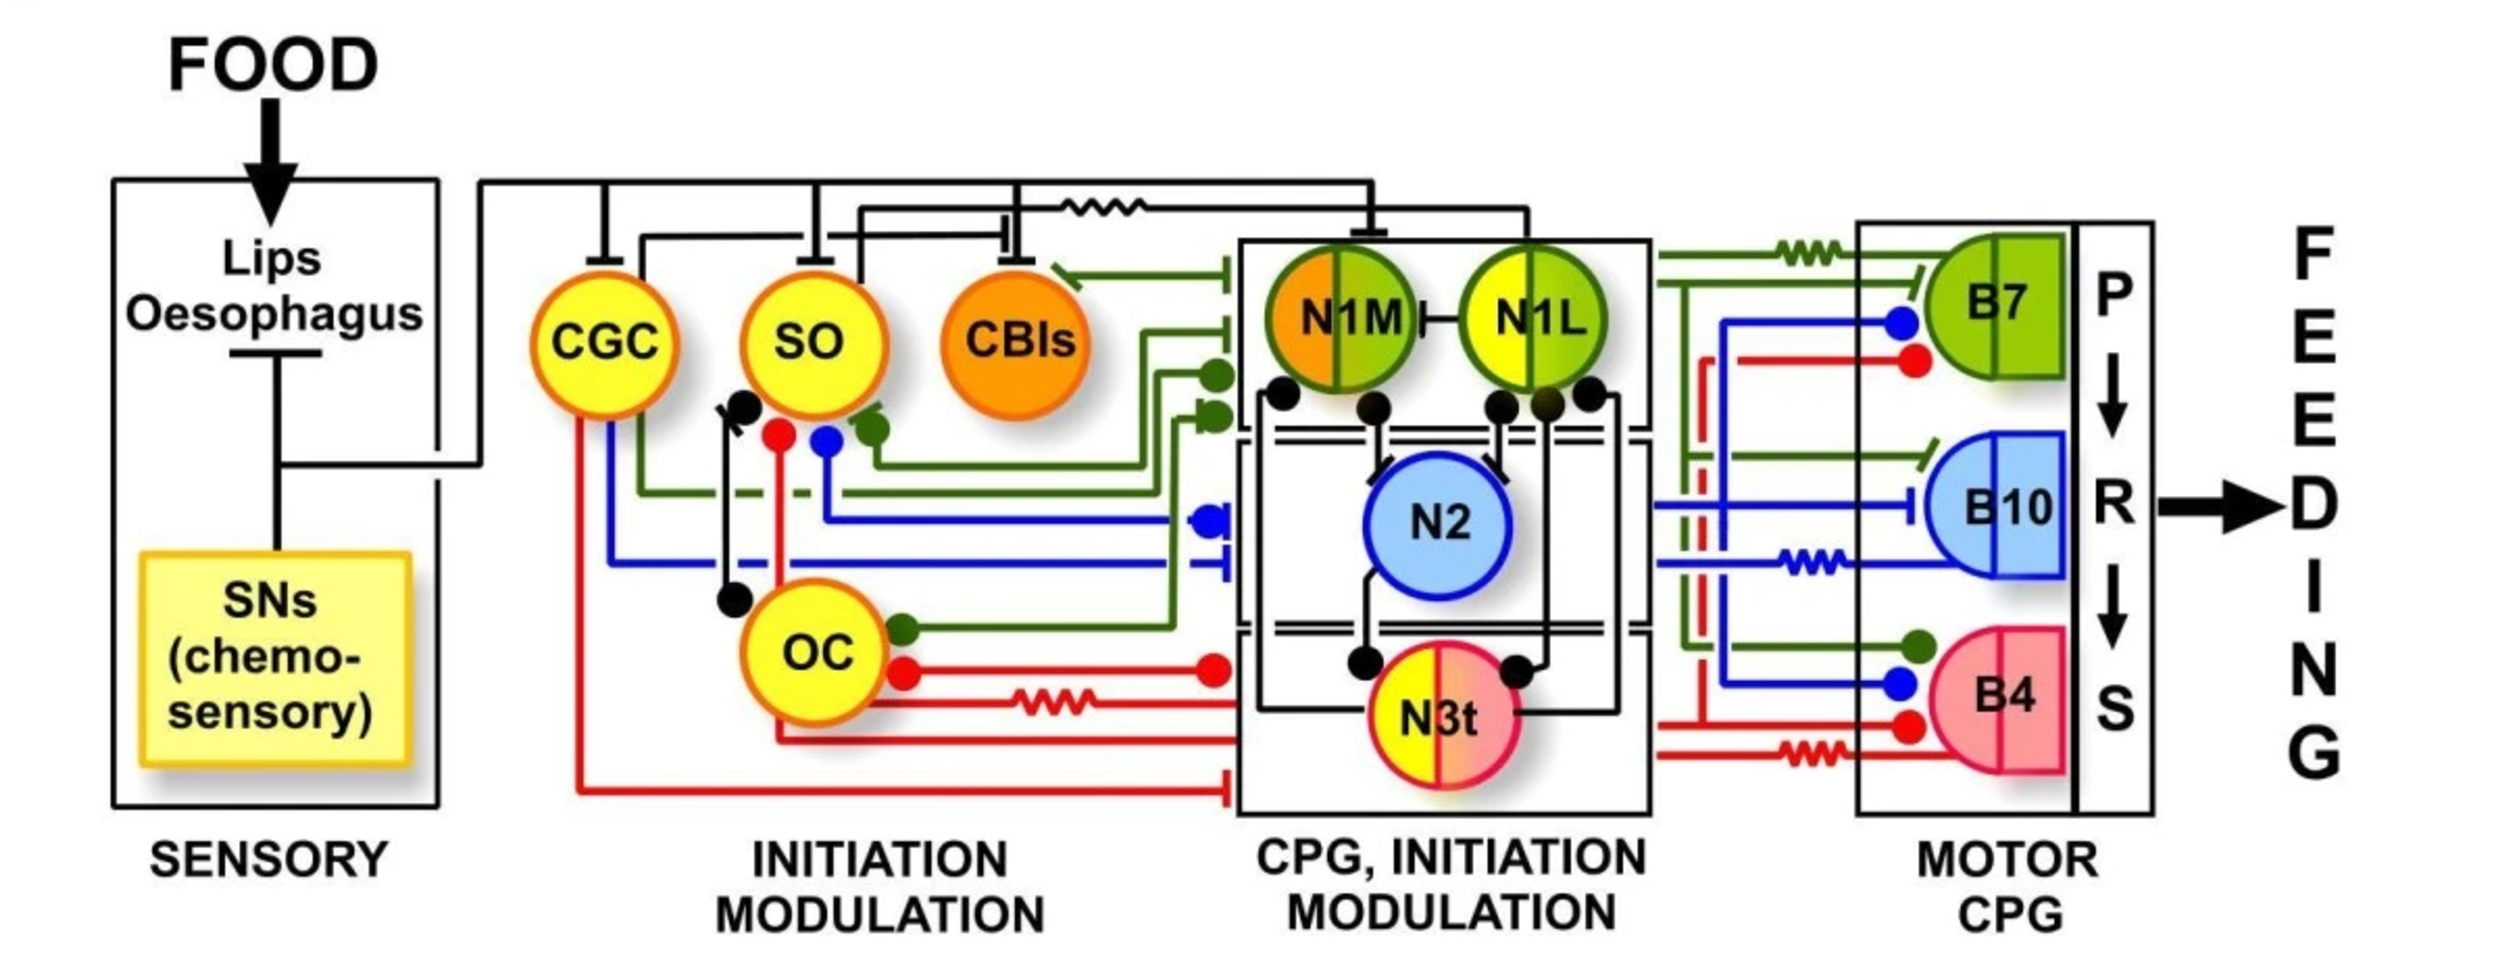
\includegraphics[width=\textwidth]{img/invariants/distributed_benjamin_2012.pdf}
	\caption{Representation of the distributed system of the feeding CPG. Dots indicate inhibitory chemical synapses, bars excitatory chemical synapses and resistor symbols electrotonic (electrical) synapses. Colors indicate the function of the neuron classified in modulatory or initiator (orange and yellow, respectively) and the three phases protraction, rasp and swallow (green, blue and red, respectively). From left to right food detection represented by Lips that stimulate CGC, SO CBIs and N1M neurons and initiate the rhythm. The ongoing activity is then modulated by those neurons but also by OC neurons and N1 and N3t neuron. Some examples of motor neurons are represented on the right side of the panel, associated to each feeding phase. This figure was adapted from Panel C from Figure 1 in \cite{benjamin_distributed_2012} (work under license \href{http://creativecommons.org/licenses/by/2.0}{Creative Commons Attribution})}
	%	Synaptic connectivity and functions of neurons in the feeding circuit. Modulatory function is indicated by yellow and initiating function by orange. CPG interneurons and motoneurons active during the three phases of the feeding rhythm are indicated by green (P = protraction), blue (R = rasp) and red (S = swallow). Neurons labeled with two colors have two functions. Dots indicate inhibitory chemical synapses, bars excitatory chemical synapses and resistor symbols electrotonic (electrical) synapses. This figure emphasizes the point that many of the neurons have more than function in the feeding network. See Abbreviations for all definitions of neuron types.
	\label{fig:feeding distribution}%
\end{figure}

%Benjamin2012    One of the central controllers of
%spontaneous feeding is the N3t CPG interneuron and
%this cell is involved in mediating the effects of hunger
%and satiety. As was described earlier, the N3ts fire toni-
%cally to inhibit the N1M cells and the rate of this tonic
%activity determines the level of activity in the whole feed-
%ing CPG. By comparing the rates of firing in isolated
%ganglia it was found that the N3t firing frequency was
%higher in satiated compared with starved snails and that
%this was inversely correlated to the frequency of sponta-
%neously fictive feeding cycles [4]. 

%kemenes 2001
%CV1a by modulating motoneuron burst duration and SO by setting the frequency of the ongoing rhythm

In this section we will analyze and describe different examples of experiments for the isolated ganglia with intracellular recordings under: spontaneous activity, SO-driven activity spontaneous and induced, medium lip nerve stimulation induced activity and CV1a-driven induced activity.



\subsection{Invariants in spontaneous activity}
The spontaneous activity here refers to intracellular recordings of the buccal ganglia after the isolation of the CNS with no chemical or electrical induced stimulation. In that case, since the CPG is able to maintain the activity in an autonomous manner, it keeps the motor activity as if the CNS was not isolated. In this case, although the characterization of the sequential dynamical invariants can be done, their possible functionality association is more complicated, since the context of the movement origin is lost. The study of these sequential restriction in artificial stimulation context can help classify this spontaneous activity, even when the rest of the system is not available. 

Here we analyze three examples of the spontaneous activity, 

\paragraph{Spontaneous Activity Example 1}
N1 phase was analyzed from B1 activity (bursting and depolarization); N2 phase was analyzed from B5 hyperpolarization, which has a strong inhibition from N2v; N3 phase was analyzed from the bursting activity of B8, that replicates the N3t duration. 

\begin{figure}[htbp]
	\centering
	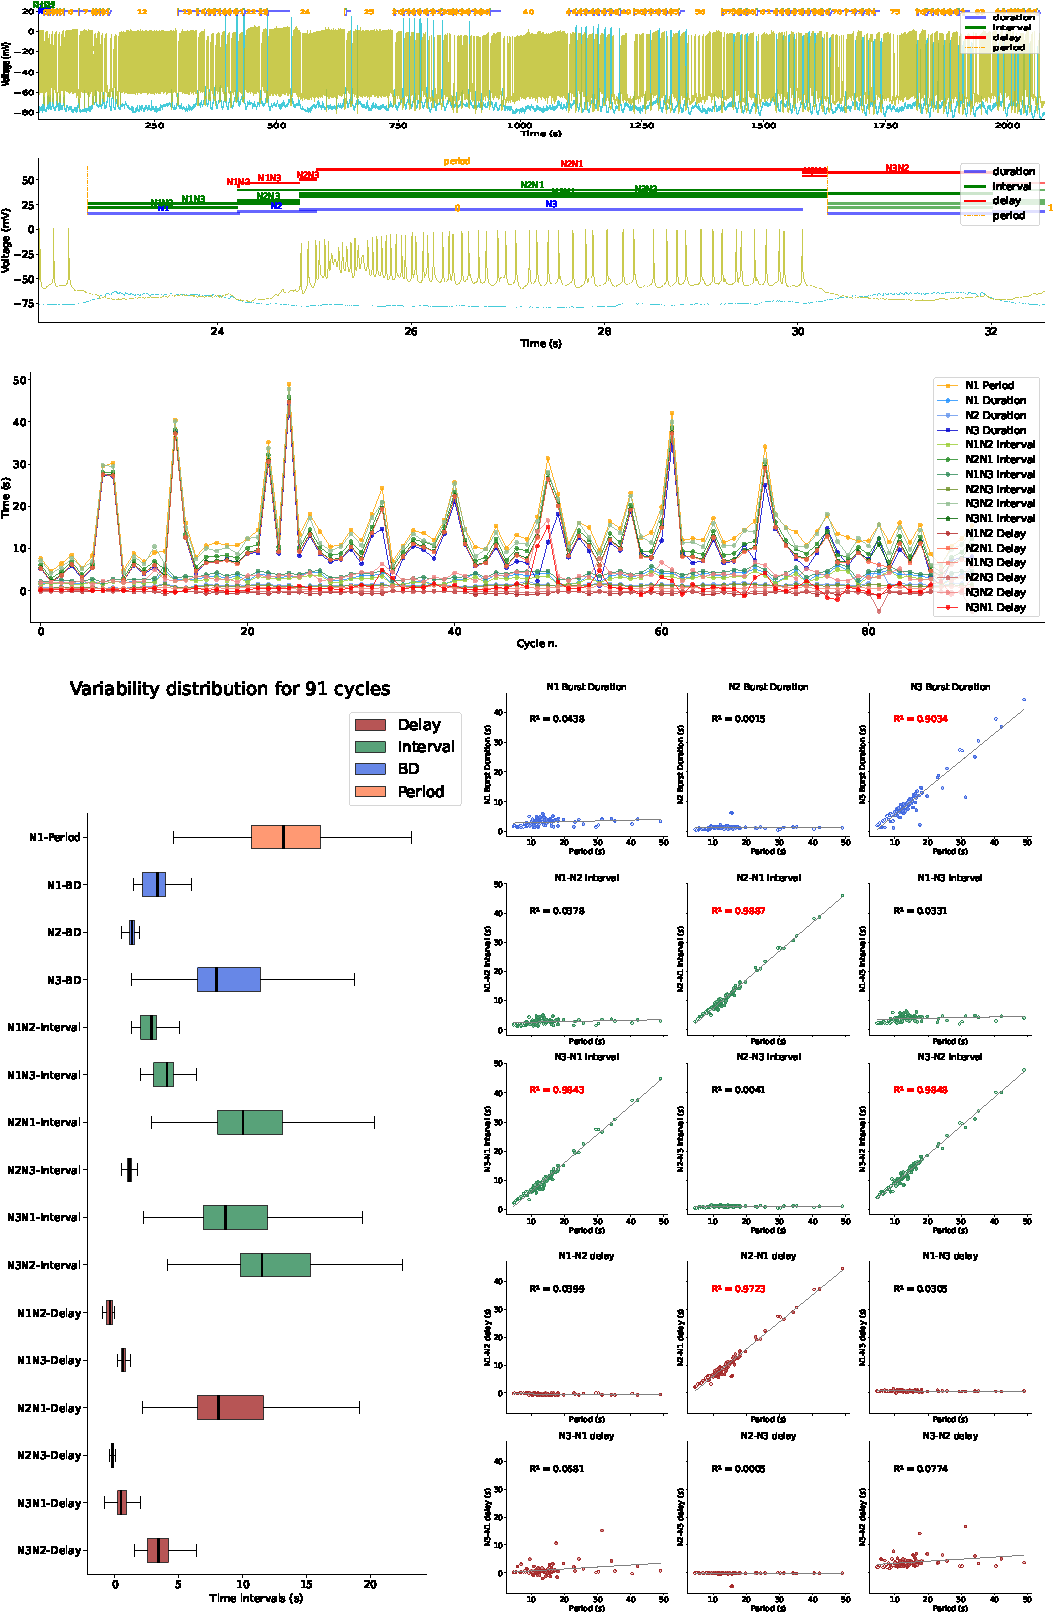
\includegraphics[width=0.9\textwidth]{./invariants/data/SUSSEX/prep2/images/3phases/panel_with_intervals.pdf}
	\caption{\textbf{Spontaneous case 1}: Panel of intervals distribution and dynamical invariants for the three phases in the CPG for spontaneous activity.}
	\label{fig:prep2 invariants}
\end{figure}

\begin{figure}[htbp]
	\centering
	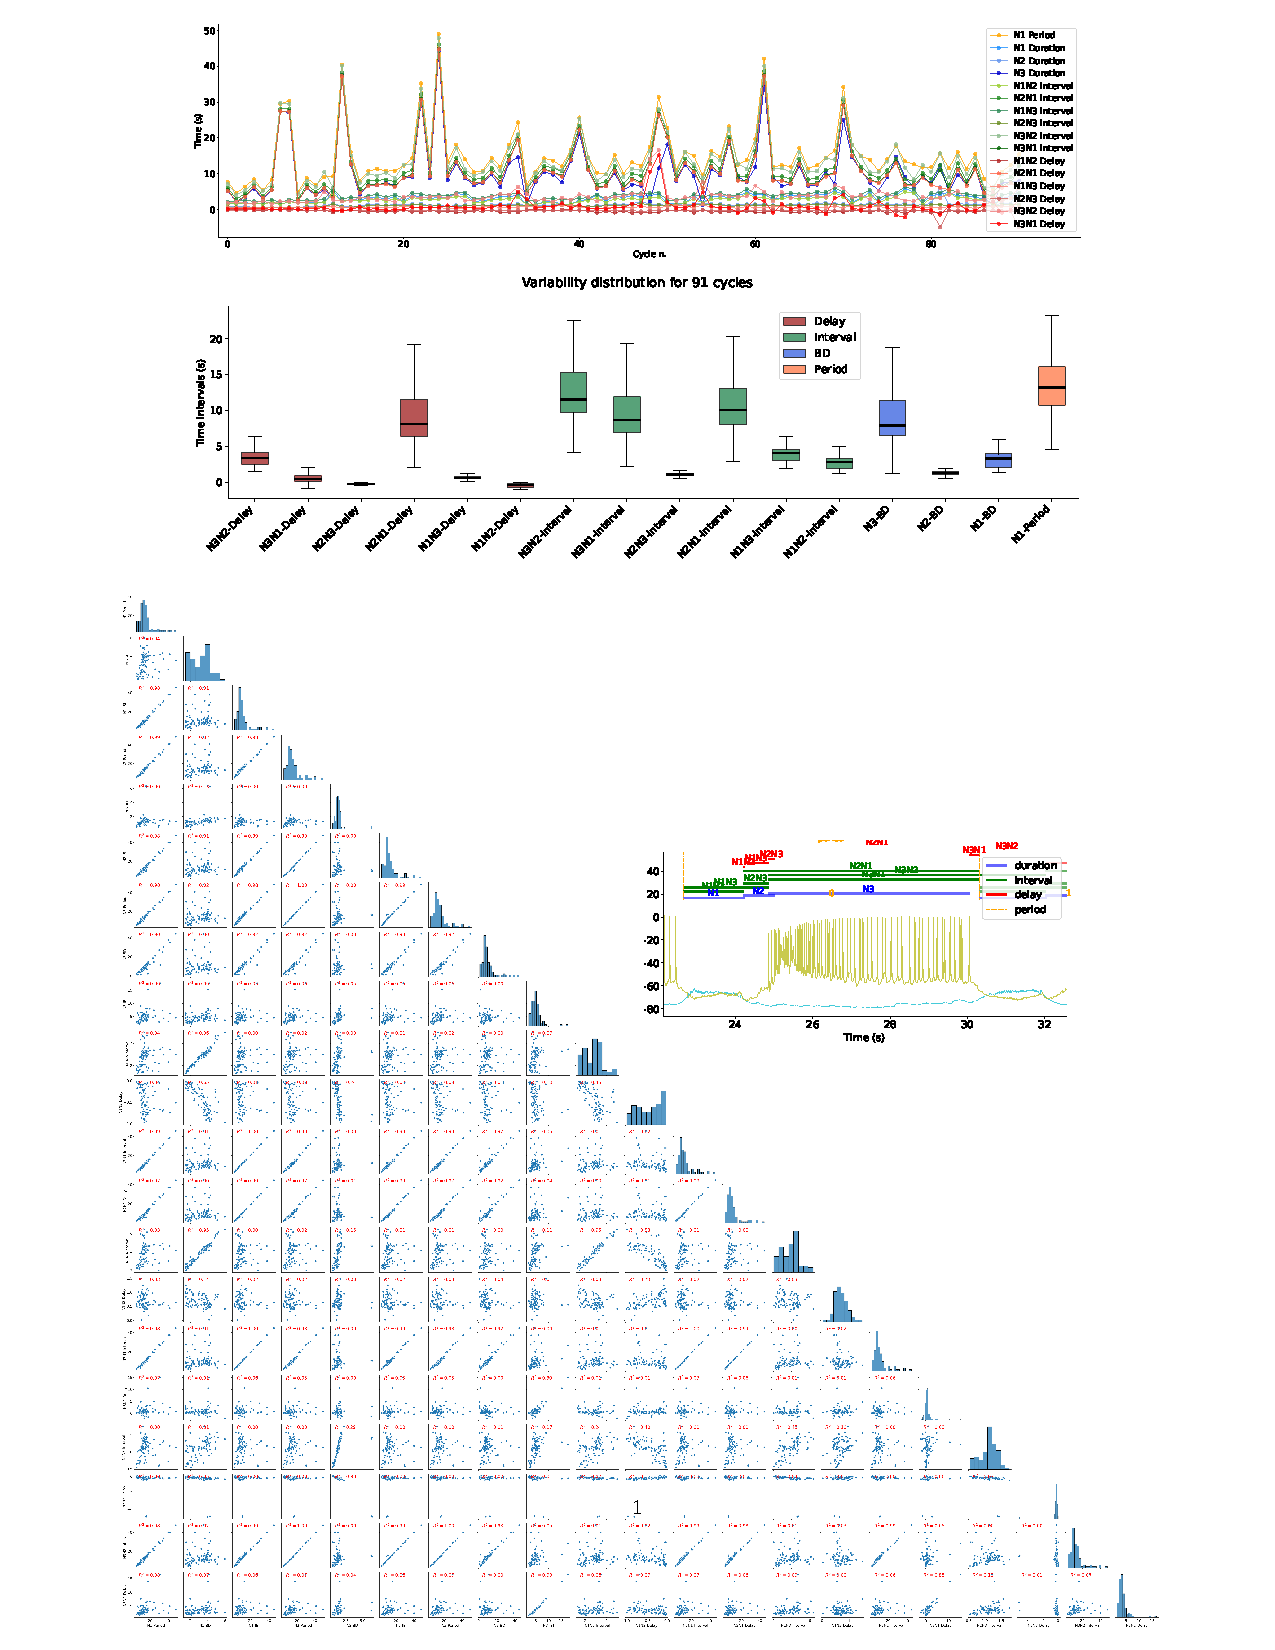
\includegraphics[width=\textwidth]{./invariants/data/SUSSEX/prep2/images/3phases/panel_with_pairplot.pdf}
	\caption{\textbf{Spontaneous case 1}: Panel of intervals distribution and dynamical invariants for the three phases in the CPG for spontaneous activity.}
	\label{fig:prep2 pairplot invariants}
\end{figure}


%\begin{figure}[htbp]
%	\centering
%	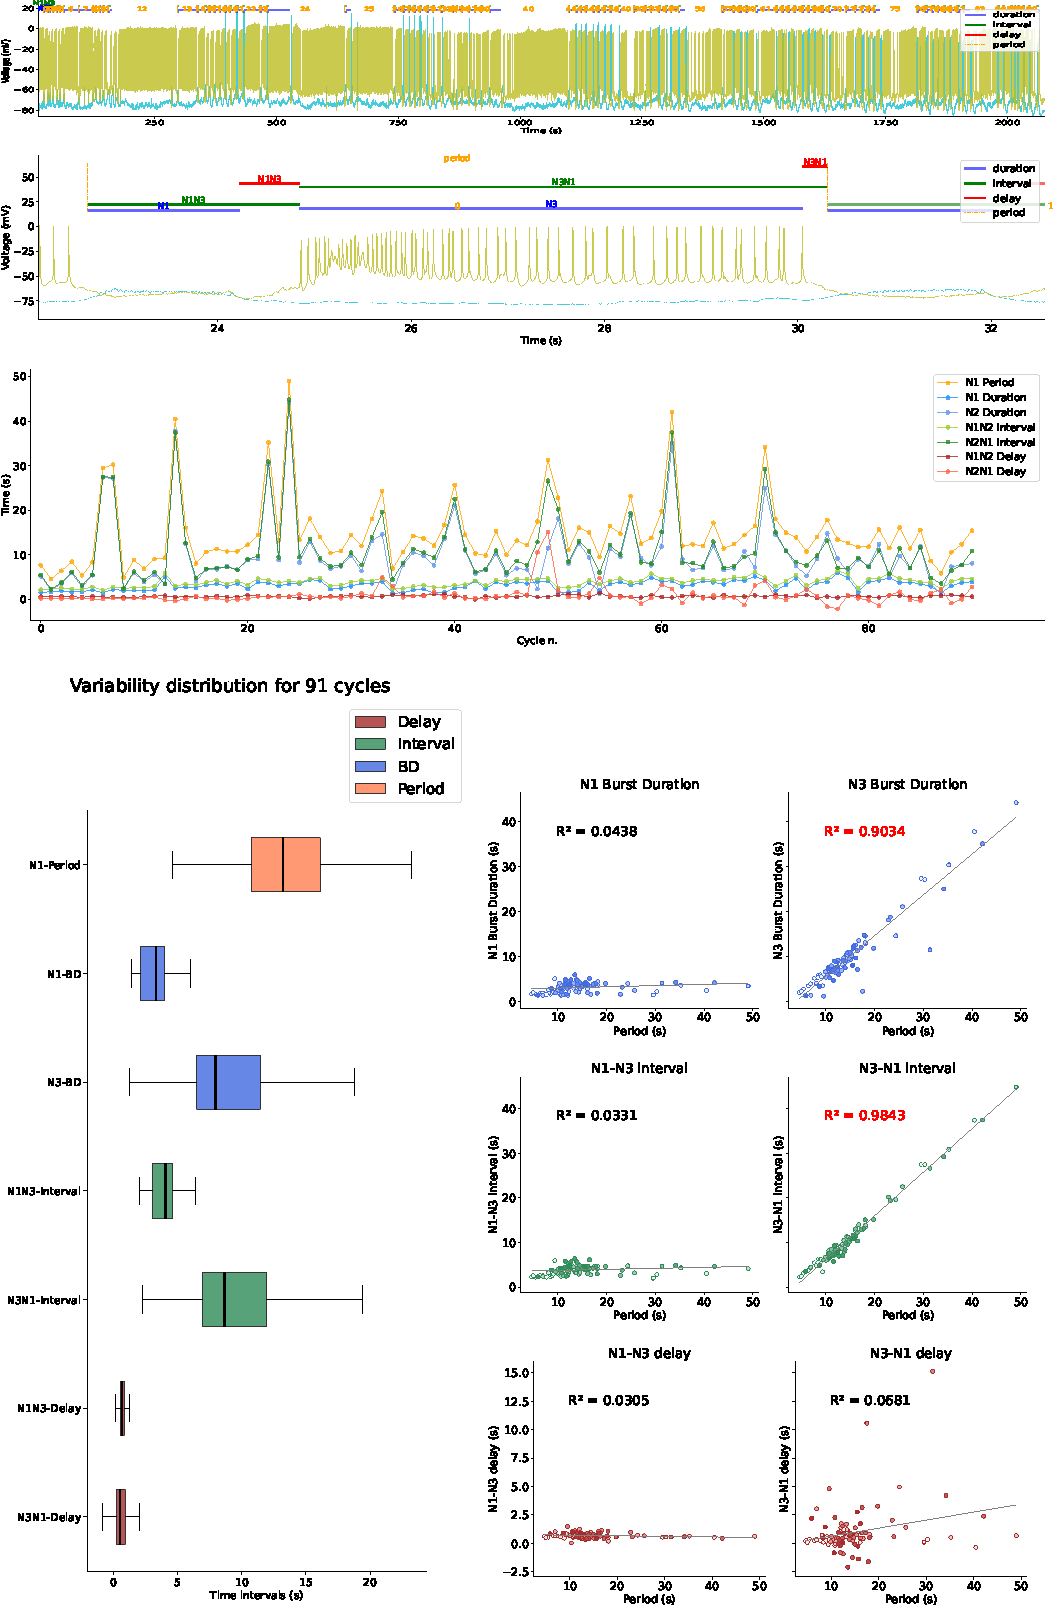
\includegraphics[width=0.9\textwidth]{./invariants/data/SUSSEX/prep2/images/2phases/panel_with_intervals.pdf}
%	\caption{\textbf{Spontaneous case2}: Panel of intervals distribution and dynamical invariants for two phases in the CPG for spontaneous activity.}
%	\label{fig:prep2 2phase invariants}
%\end{figure}
%
%\begin{figure}[htbp]
%\centering
%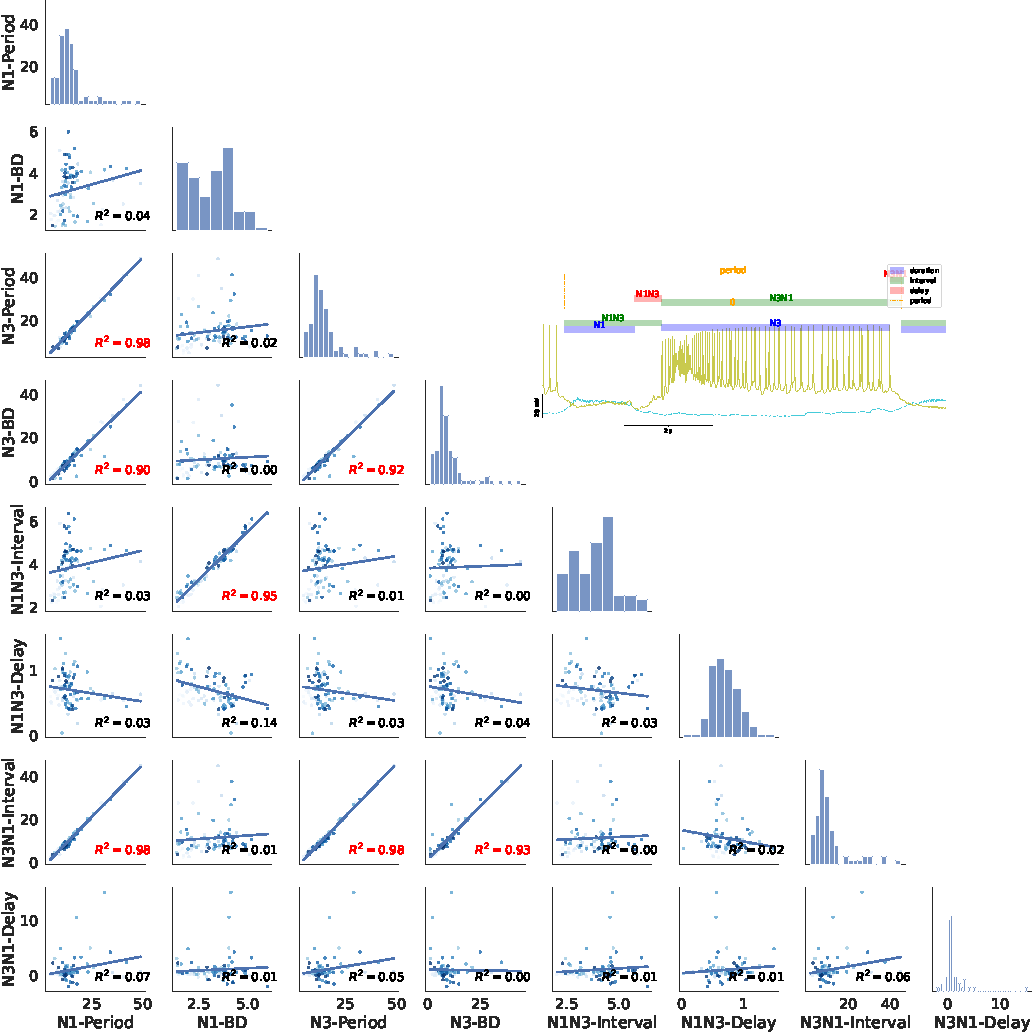
\includegraphics[width=0.9\textwidth]{./invariants/data/SUSSEX/prep2/images/2phases/panel_with_pairplot.pdf}
%\caption{\textbf{Spontaneous case2}: Panel of intervals distribution and dynamical invariants for two phases in the CPG for spontaneous activity.}
%\label{fig:prep2 2phase invariants pairplot}
%\end{figure}

\paragraph{Spontaneous Activity Example 2}
N1 phase was analyzed from B1 activity (bursting and depolarization); N2 phase was analyzed from B1 hyperpolarization, which has a strong inhibition from N2v; N3 phase was analyzed from the bursting activity of B8, that replicates the N3t duration. 
Since the reference for N2 here coincides with N1 reference, we display here only the intervals corresponding to N1 and N3 phases, since the intervals that correspond to 3 phases, such as N1-N2 delay or N2-N3 delay, either are already represented in the defined intervals or have a duration close to 0 ms.

\begin{figure}[htbp]
	\centering
	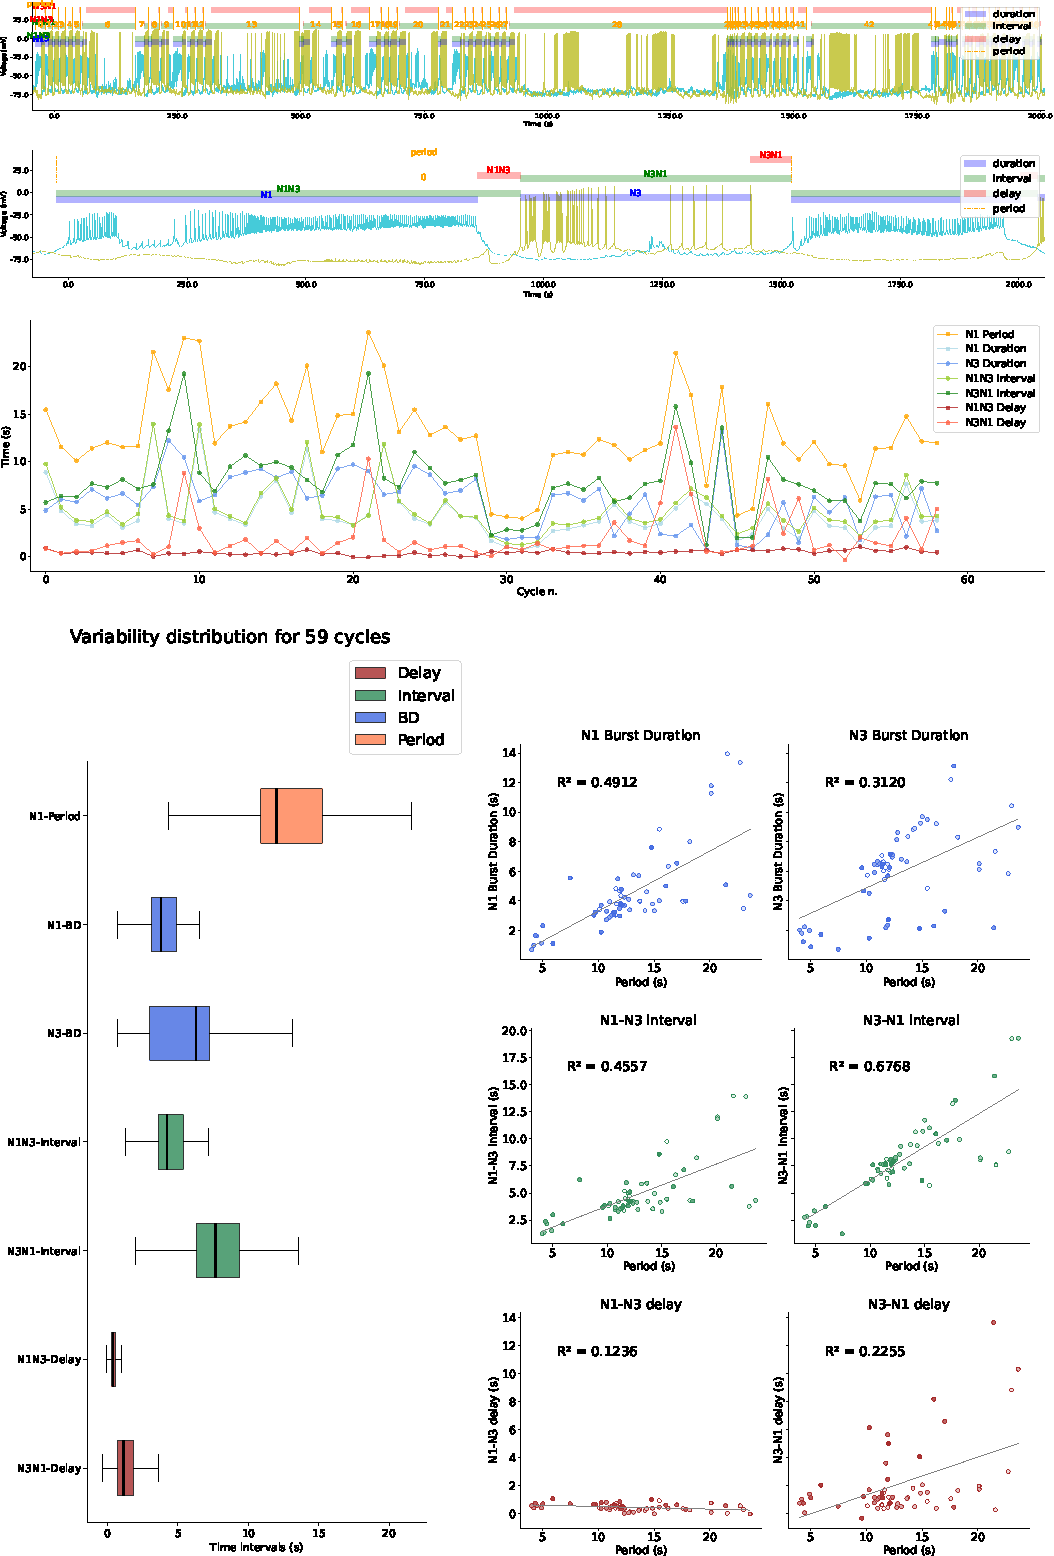
\includegraphics[width=0.9\textwidth]{./invariants/data/SUSSEX/prep3/images/2phases/panel_with_intervals.pdf}
	\caption{\textbf{Spontaneous case 2}: Panel of intervals distribution and dynamical invariants for two phases in the CPG for spontaneous activity.}
	\label{fig:prep3 2phases invariants}
\end{figure}

\begin{figure}[htbp]
	\centering
	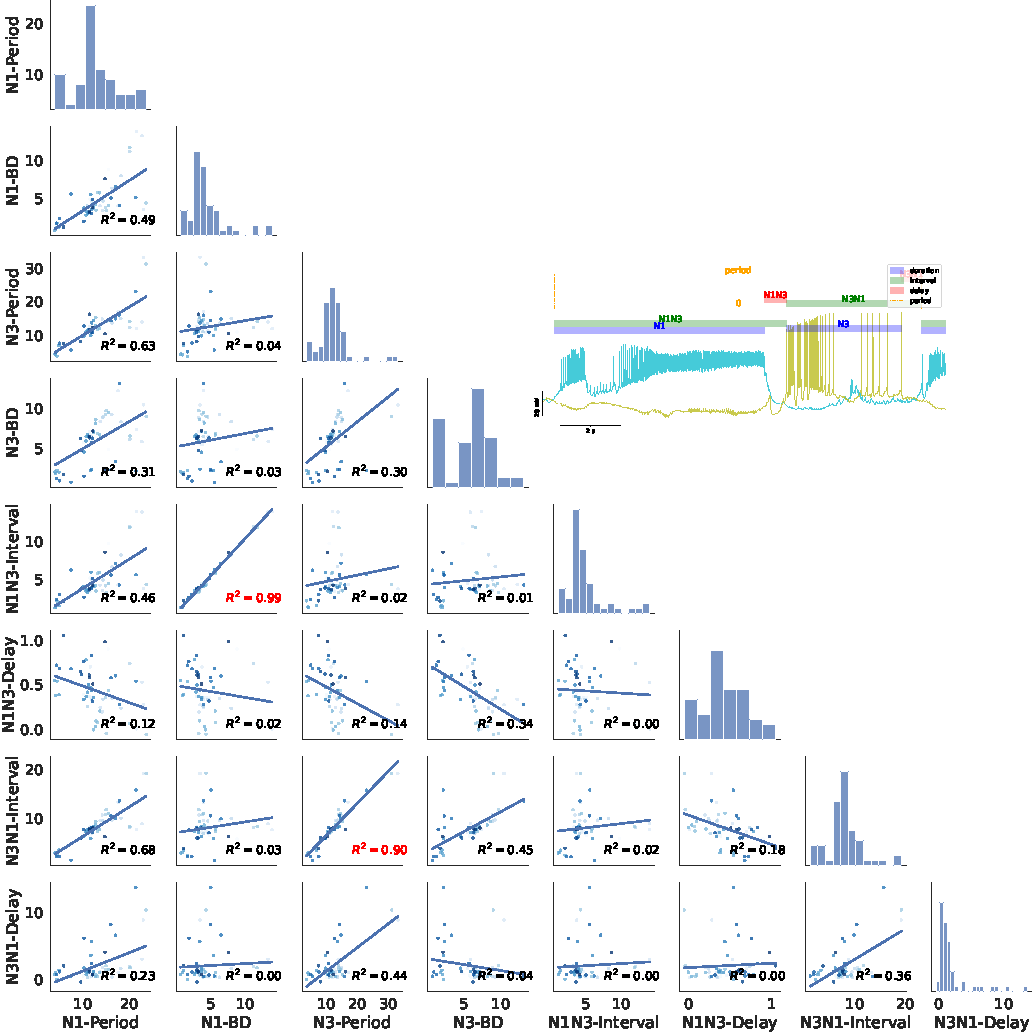
\includegraphics[width=0.9\textwidth]{./invariants/data/SUSSEX/prep3/images/2phases/panel_with_pairplot.pdf}
	\caption{\textbf{Spontaneous case 2}: Panel of intervals distribution and dynamical invariants for two phases in the CPG for spontaneous activity.}
	\label{fig:prep3 2phases invariants pairplot}
\end{figure}

%\begin{figure}[htbp]
%	\centering
%	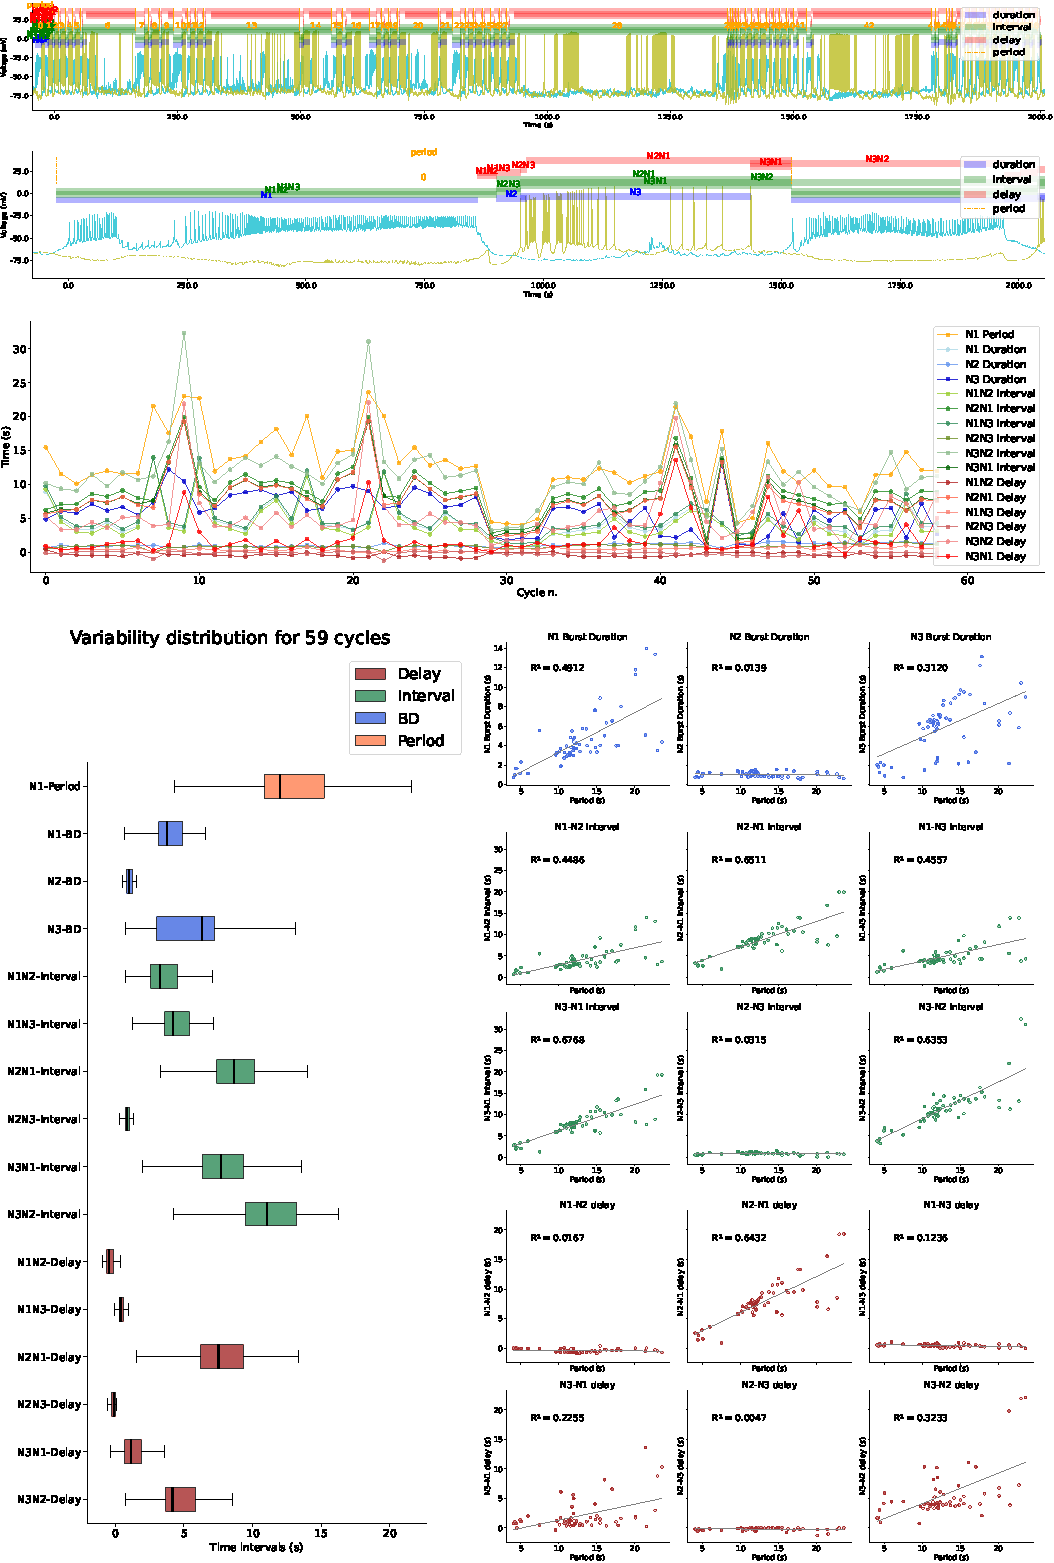
\includegraphics[width=0.9\textwidth]{./invariants/data/SUSSEX/prep3/images/3phases/panel_with_intervals.pdf}
%	\caption{\textbf{Spontaneous case3}: Panel of intervals distribution and dynamical invariants for the three phases in the CPG for spontaneous activity.}
%	\label{fig:prep3 invariants}
%\end{figure}
%
%\begin{figure}[htbp]
%	\centering
%	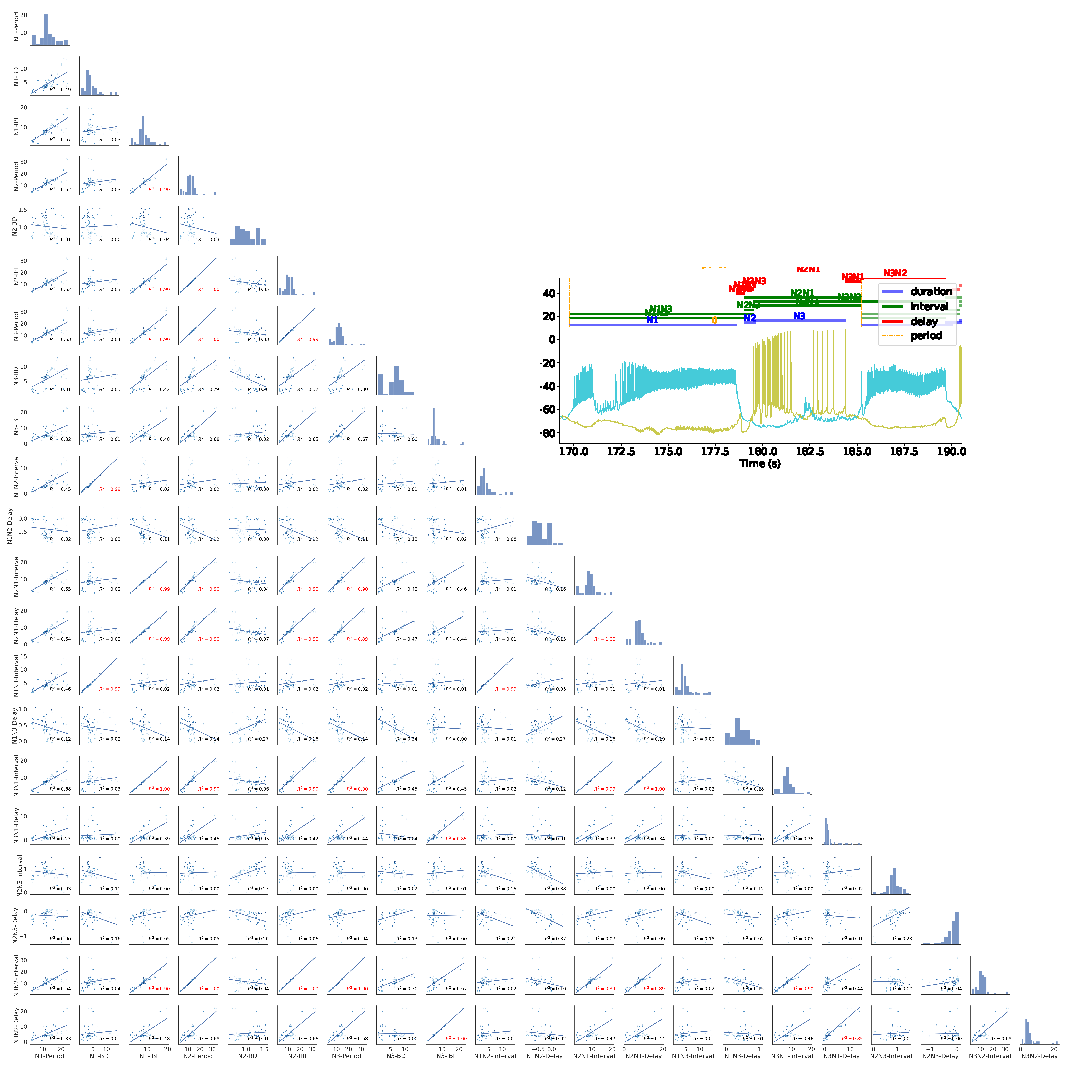
\includegraphics[width=0.9\textwidth]{./invariants/data/SUSSEX/prep3/images/3phases/panel_with_pairplot.pdf}
%	\caption{\textbf{Spontaneous case3}: Panel of intervals distribution and dynamical invariants for the three phases in the CPG for spontaneous activity.}
%	\label{fig:prep3 invariants pairplot}
%\end{figure}


\paragraph{Spontaneous Activity Example 3}
N1 phase was analyzed from B1 activity (bursting and depolarization); N2 phase was analyzed from B5 hyperpolarization, which has a strong inhibition from N2v; N3 phase was analyzed from the bursting activity of B8, that replicates the N3t duration. 

\begin{figure}[htbp]
	\centering
	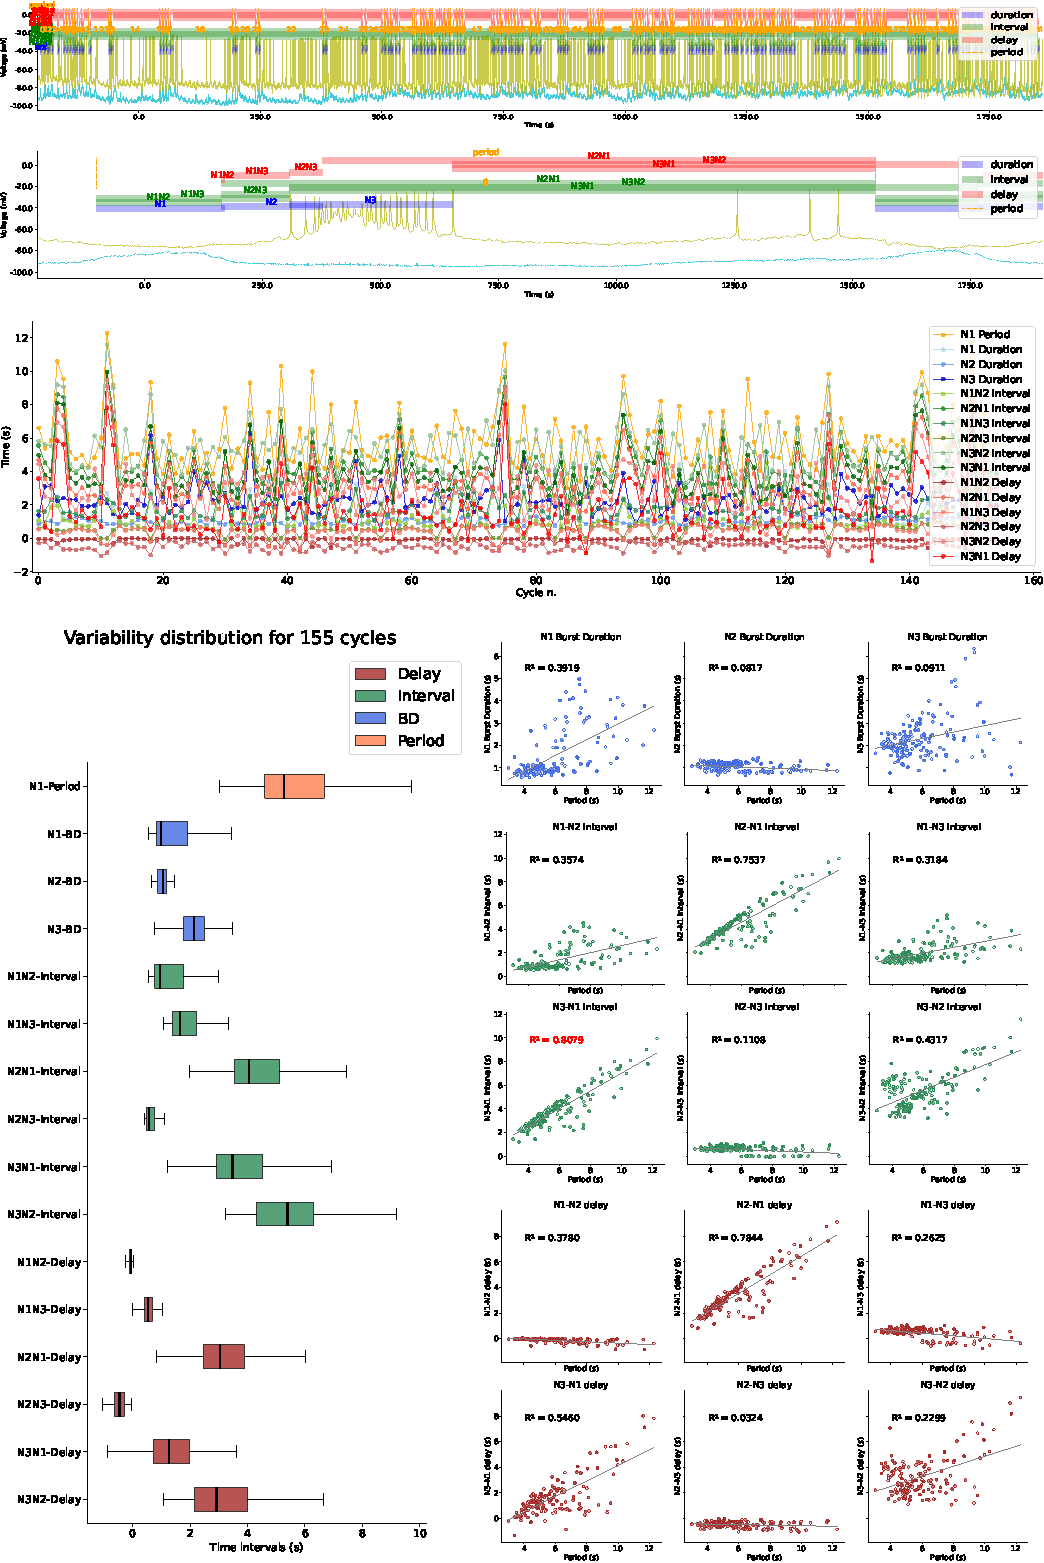
\includegraphics[width=0.9\textwidth]{./invariants/data/SUSSEX/prep1/images/3phases/panel_with_intervals.pdf}
	\caption{\textbf{Spontaneous case 3}: Panel of intervals distribution and dynamical invariants for the three phases in the CPG for spontaneous activity.}
	\label{fig:prep1 invariants}
\end{figure}


\begin{figure}[htbp]
	\centering
	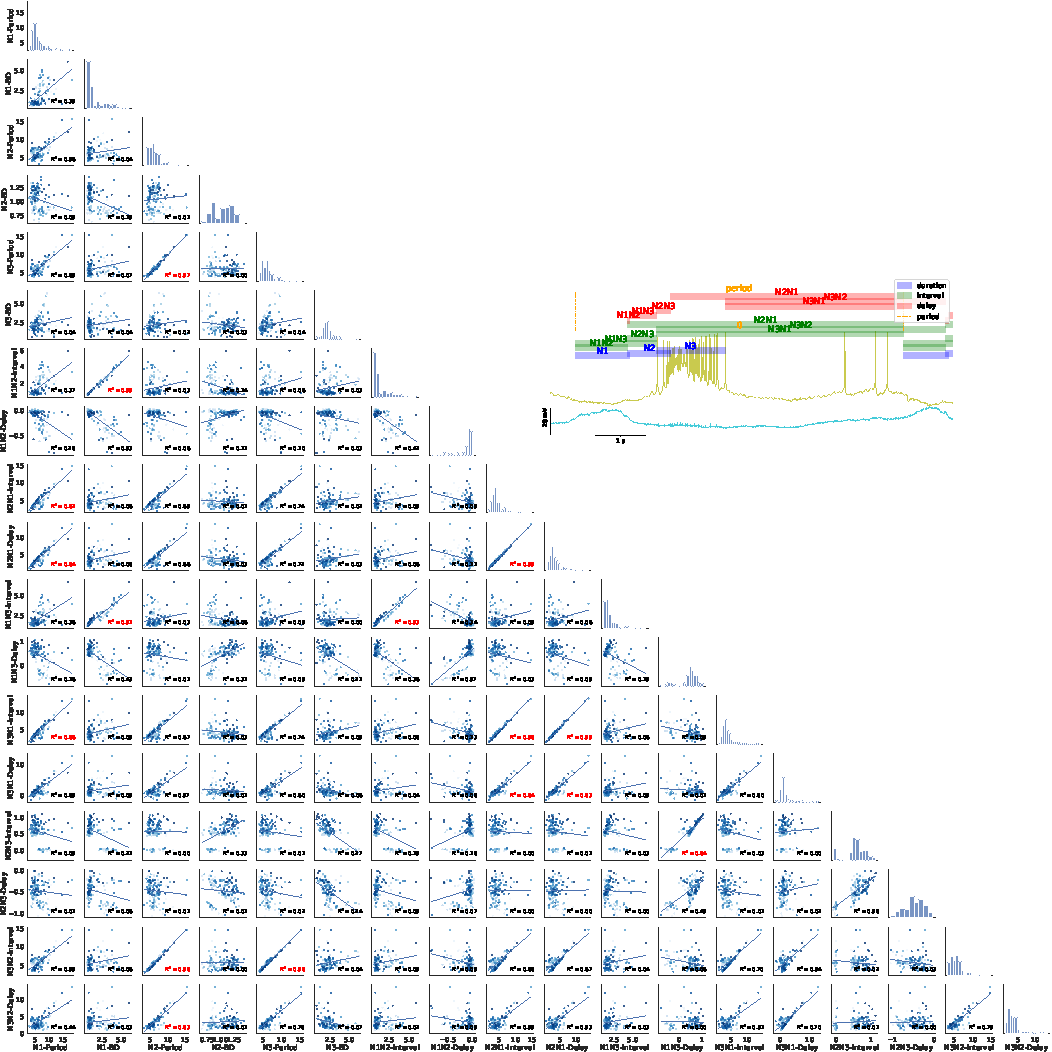
\includegraphics[width=\textwidth]{./invariants/data/SUSSEX/prep1/images/3phases/panel_with_pairplot.pdf}
	\caption{\textbf{Spontaneous case 3}: Panel of intervals distribution and dynamical invariants for the three phases in the CPG for spontaneous activity.}
	\label{fig:prep1 invariants pairplot}
\end{figure}

%
%\begin{figure}[htbp]
%	\centering
%	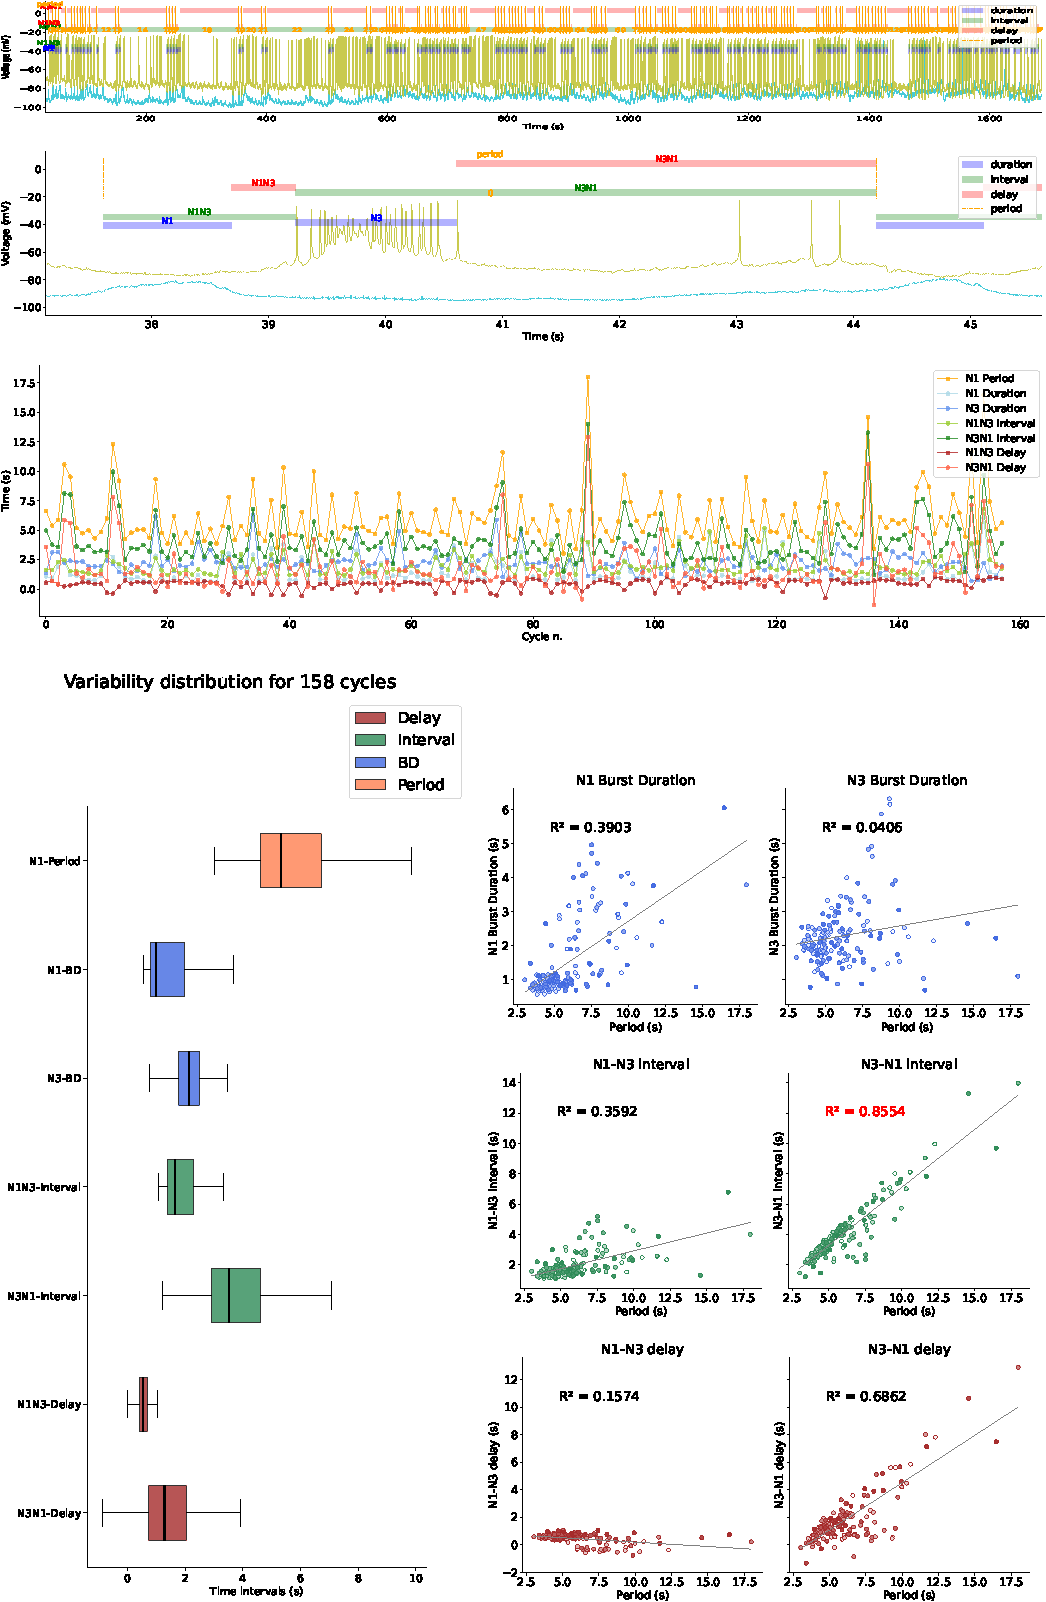
\includegraphics[width=0.9\textwidth]{./invariants/data/SUSSEX/prep1/images/2phases/panel_with_intervals.pdf}
%	\caption{\textbf{Spontaneous case1}: Panel of intervals distribution and dynamical invariants for two phases in the CPG for spontaneous activity.}
%	\label{fig:prep1 2 phases invariants}
%\end{figure}
%%
%\begin{figure}[htbp]
%	\centering
%	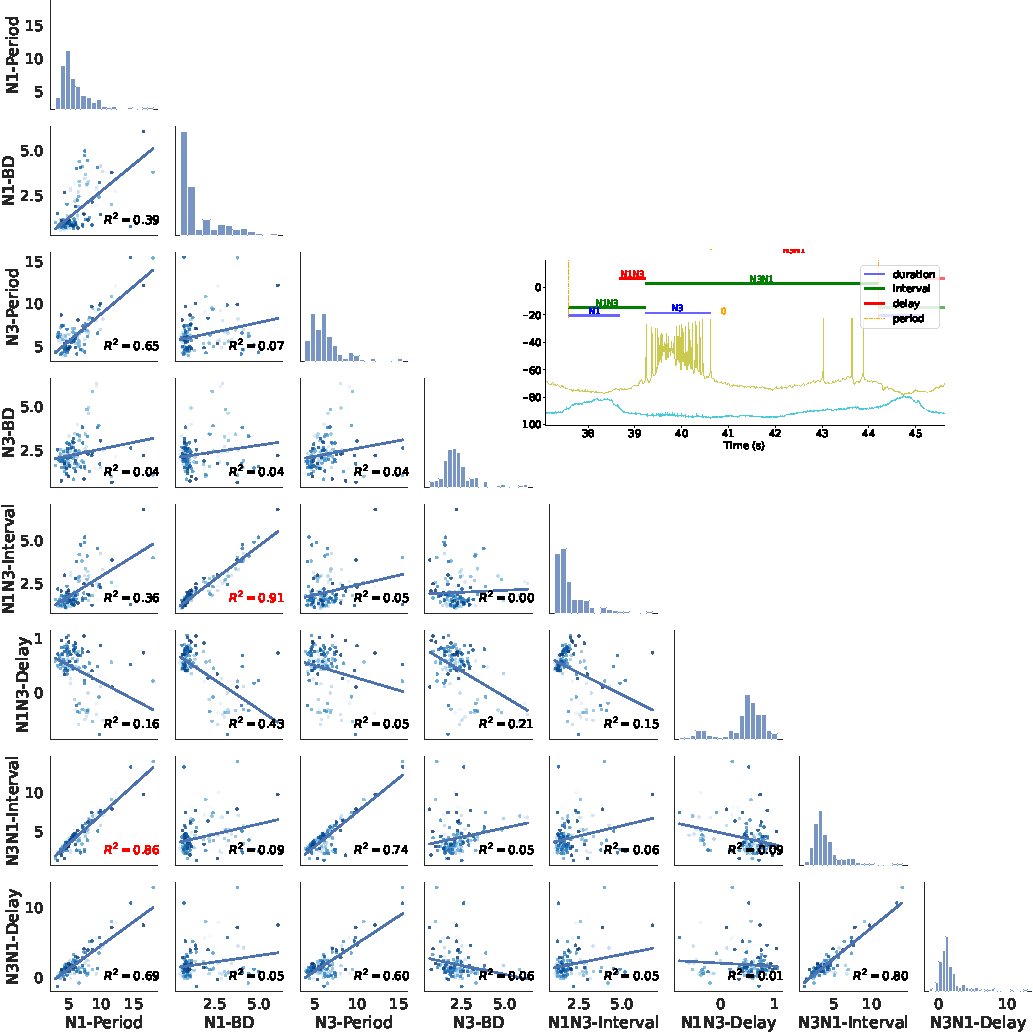
\includegraphics[width=0.9\textwidth]{./invariants/data/SUSSEX/prep1/images/2phases/panel_with_pairplot.pdf}
%	\caption{\textbf{Spontaneous case1}: Panel of intervals distribution and dynamical invariants for the two phases in the CPG for spontaneous activity.}
%	\label{fig:prep1 2 phases invariants pairplot}
%\end{figure}




\subsection{Invariants in SO driven activity}
\paragraph{1. Spontaneous SO modulation recording}
% Nota: datos de preparación 4 en la detección está solo n1m y b8, las fases son N1 y N3. 
 
\begin{figure}[htbp]
	\centering
	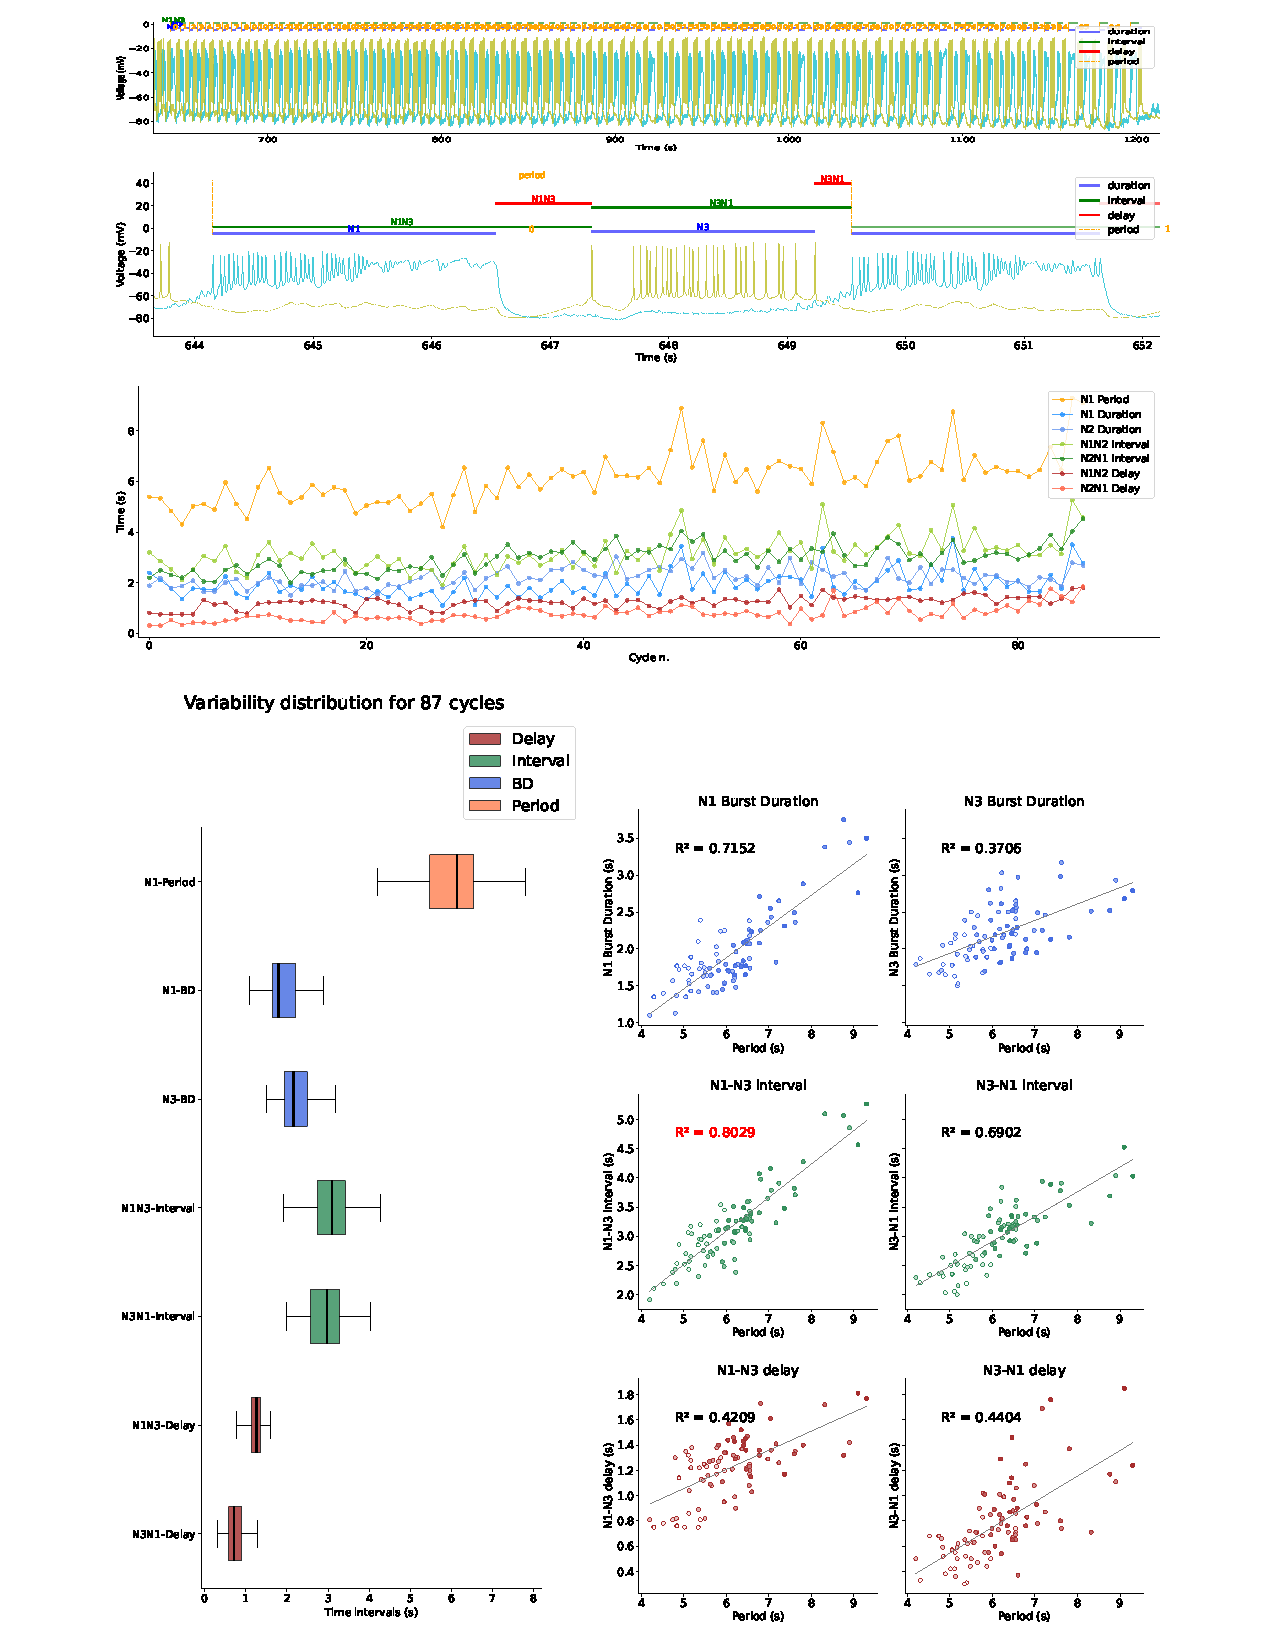
\includegraphics[width=0.9\textwidth]{./invariants/data/SUSSEX/prep4_so_driven_2/images/panel_with_intervals.pdf}
	\caption{\textbf{Spontaneous SO neuron driven}: Panel of intervals distribution and dynamical invariants for the two phases in the CPG for spontaneous activity driven by SO neuron.}
	\label{fig:so spontaneous invariants}
\end{figure}

\begin{figure}[htbp]
	\centering
	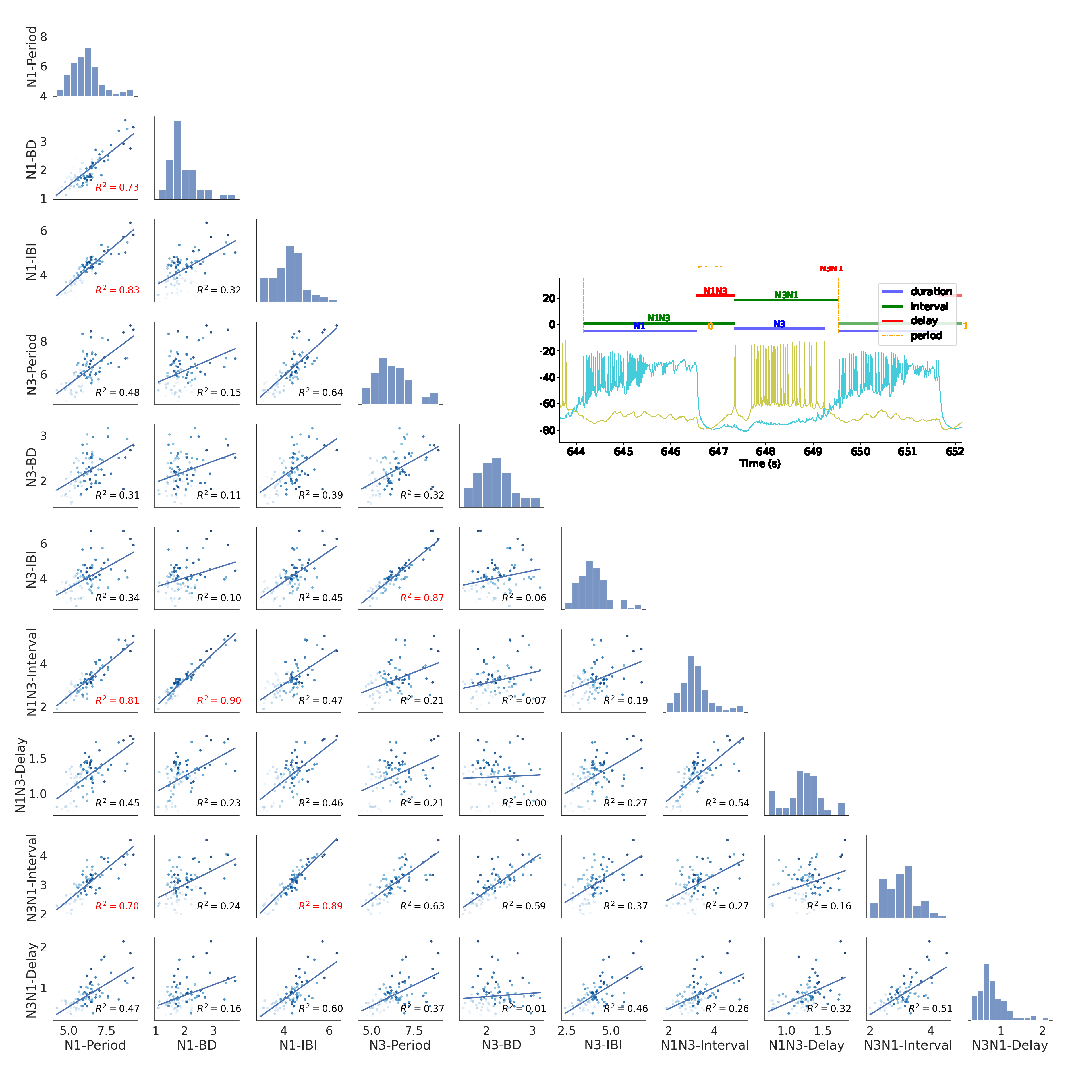
\includegraphics[width=0.9\textwidth]{./invariants/data/SUSSEX/prep4_so_driven_2/images/panel_with_pairplot.pdf}
	\caption{\textbf{Spontaneous SO neuron driven}: Panel of intervals distribution and dynamical invariants for the two phases in the CPG for spontaneous activity driven by SO neuron.}
	\label{fig:so spontaneous invariants pairplot}
\end{figure}
 	


\begin{figure}[htbp]
	\centering
	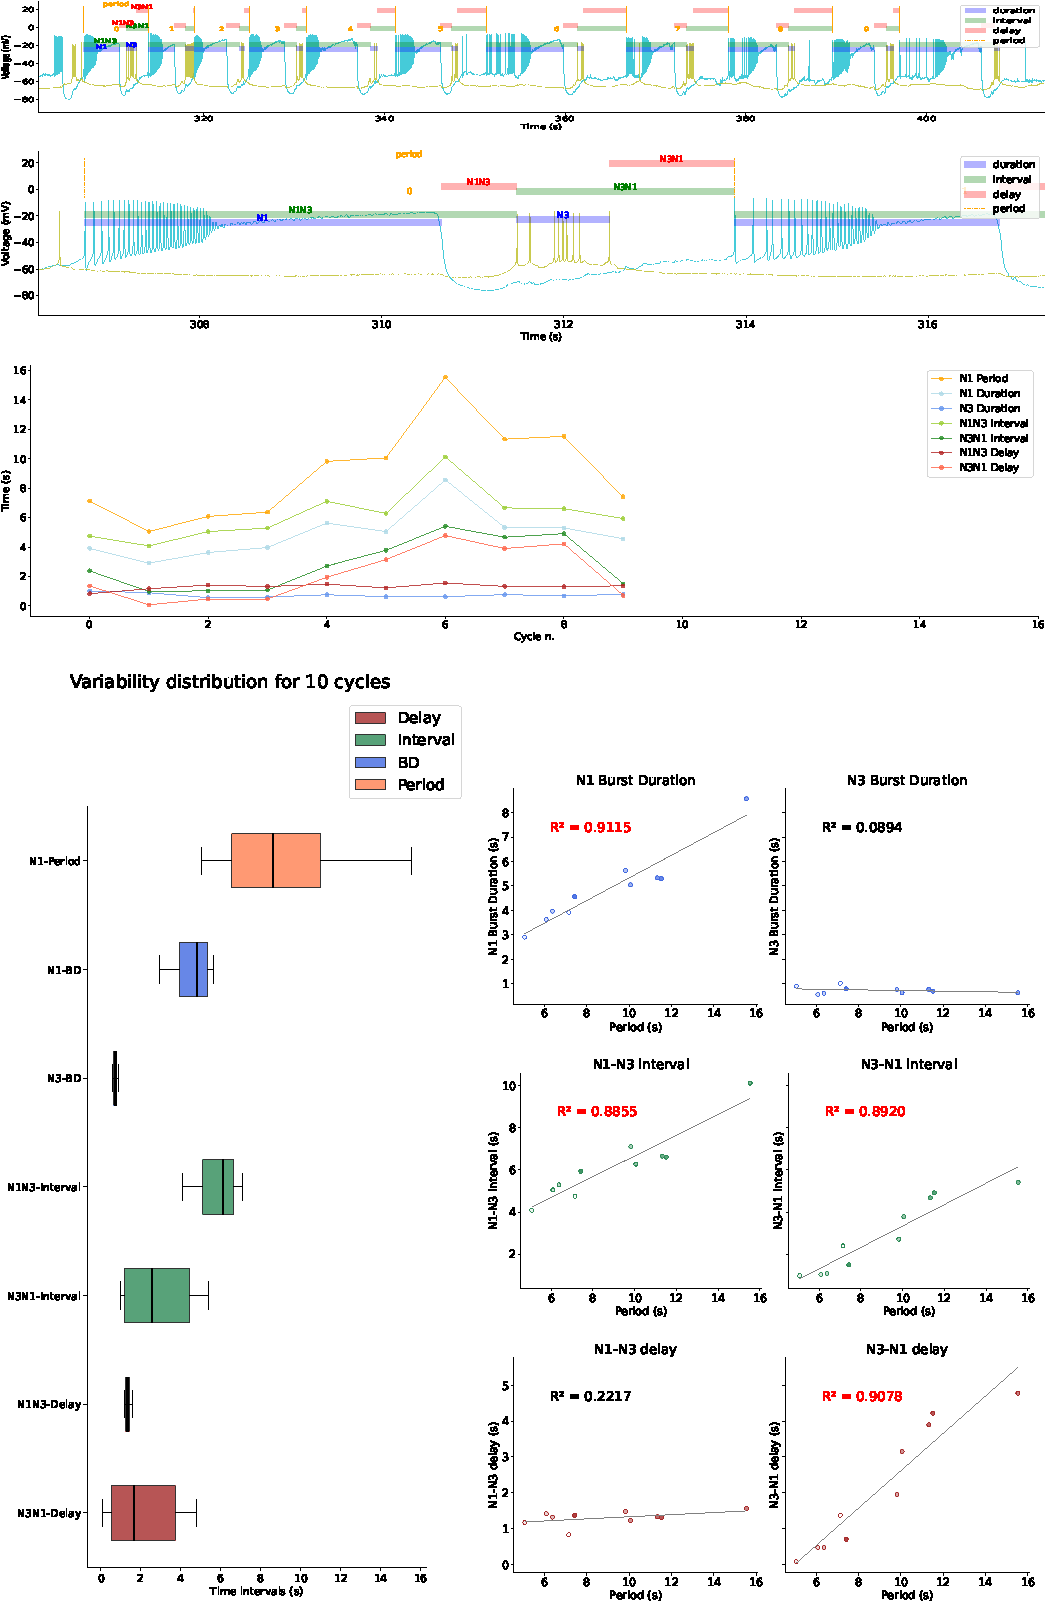
\includegraphics[width=0.9\textwidth]{./invariants/data/SUSSEX/prep4_so_no_driven/images/panel_with_intervals.pdf}
	\caption{\textbf{Spontaneous activity when SO-driven is over}: Panel of intervals distribution and dynamical invariants for the three phases in the CPG for spontaneous activity.}
	\label{fig:no so spontaneous invariants}
\end{figure}
 	 
 
\begin{figure}[htbp]
	\centering
	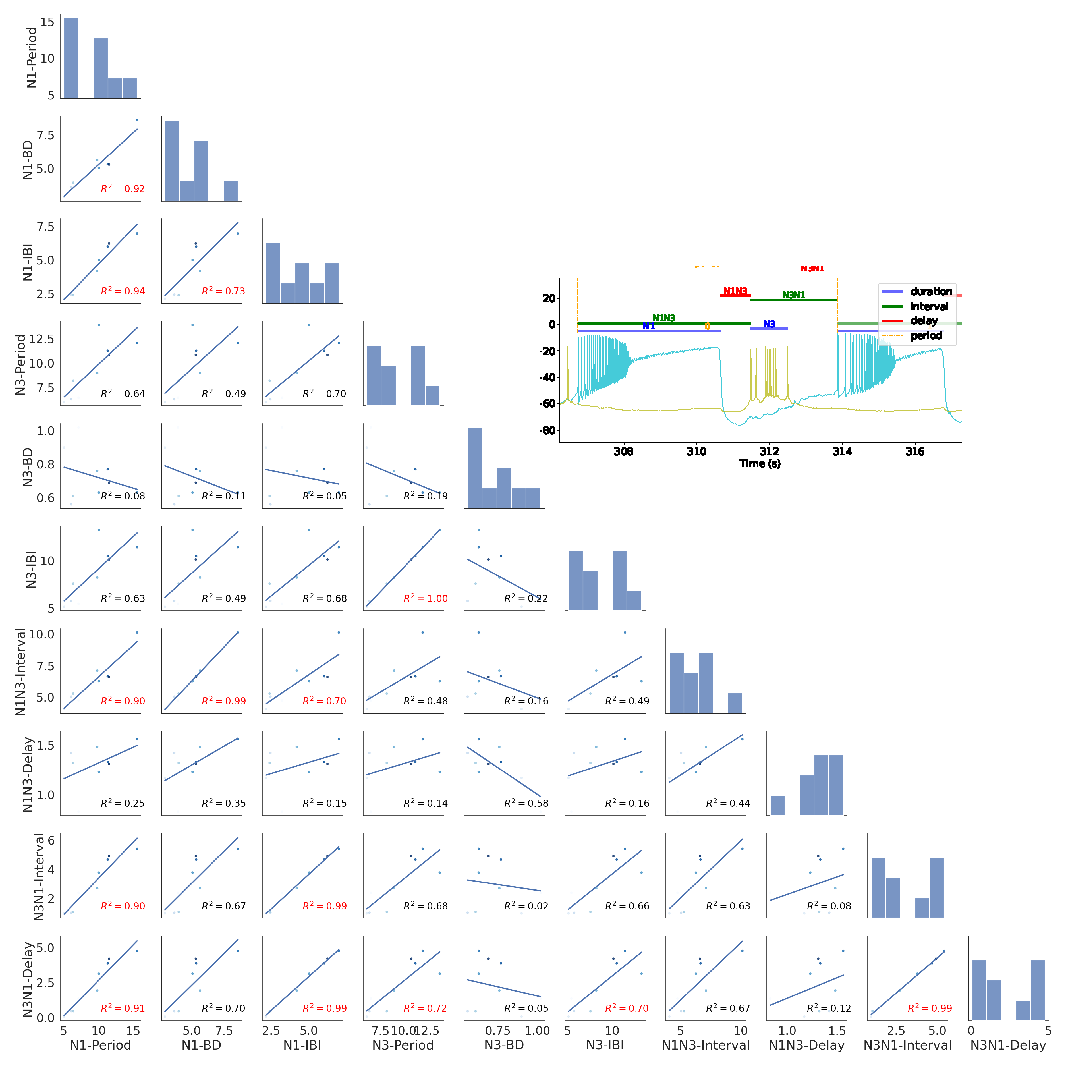
\includegraphics[width=0.9\textwidth]{./invariants/data/SUSSEX/prep4_so_no_driven/images/panel_with_pairplot.pdf}
	\caption{\textbf{Spontaneous activity when SO-driven is over}: Panel of intervals distribution and dynamical invariants for the three phases in the CPG for spontaneous activity.}
	\label{fig:no so spontaneous invariants pairplot}
\end{figure}
 
\paragraph{2. Stimulated SO recording}


\begin{figure}[htbp]
	\centering
	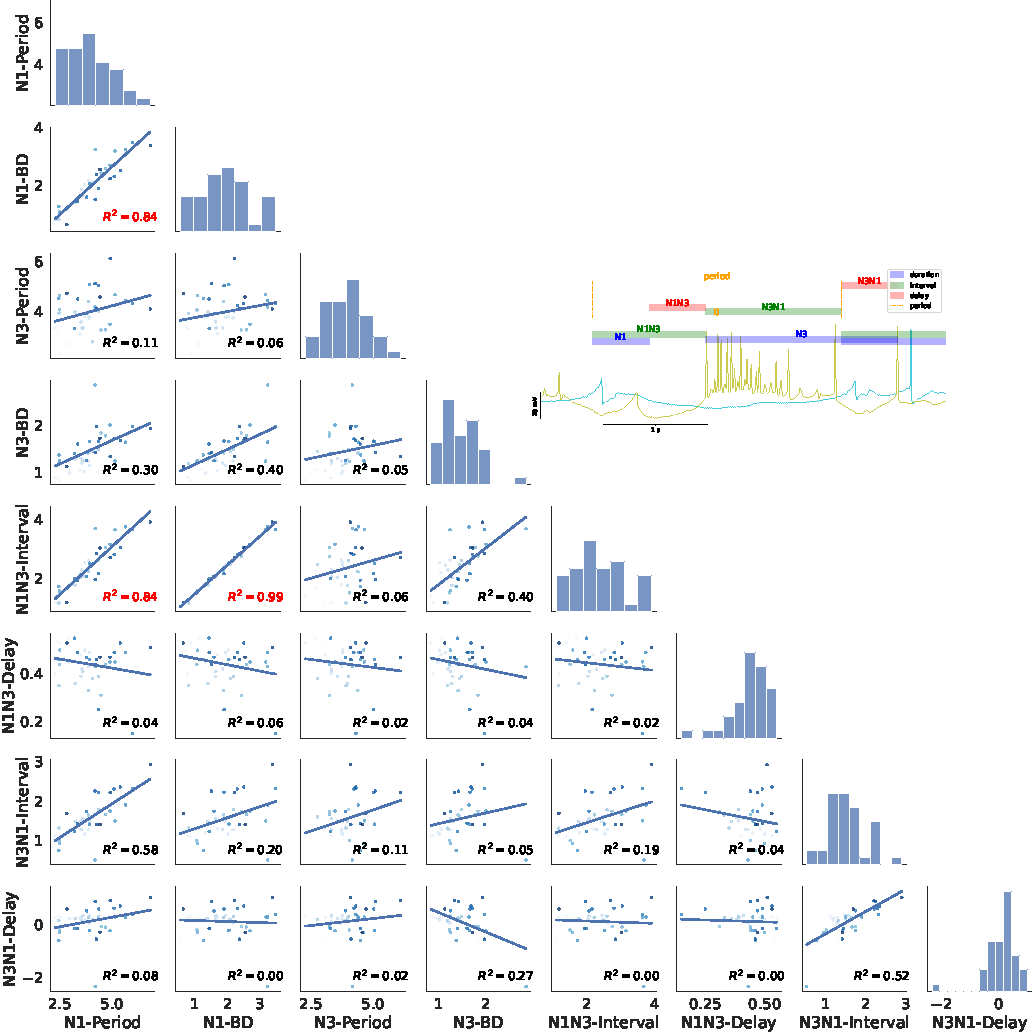
\includegraphics[width=0.9\textwidth]{./invariants/data/SUSSEX/SO_driven/images/panel_with_pairplot.pdf}
	\caption{\textbf{SO driven stimulation}: Panel of intervals distribution and dynamical invariants for the three phases in the CPG under SO modulatory neuron stimulation.}
	\label{fig:so stimulation pairplot}
\end{figure}



\subsection{Invariants in MLN stimulation driven activity}
The snail's lips are connected to the cerebral ganglia by the MLN (median lip nerves). It is possible to stimulate CPG activity by its stimulation, simulating the initiation of the rhythm in food presence \parencite{staras_electrophysiological_2019}. The data in this recording was stimulated by (4volt 1Hz stim).


\begin{figure}[htbp]
	\centering
	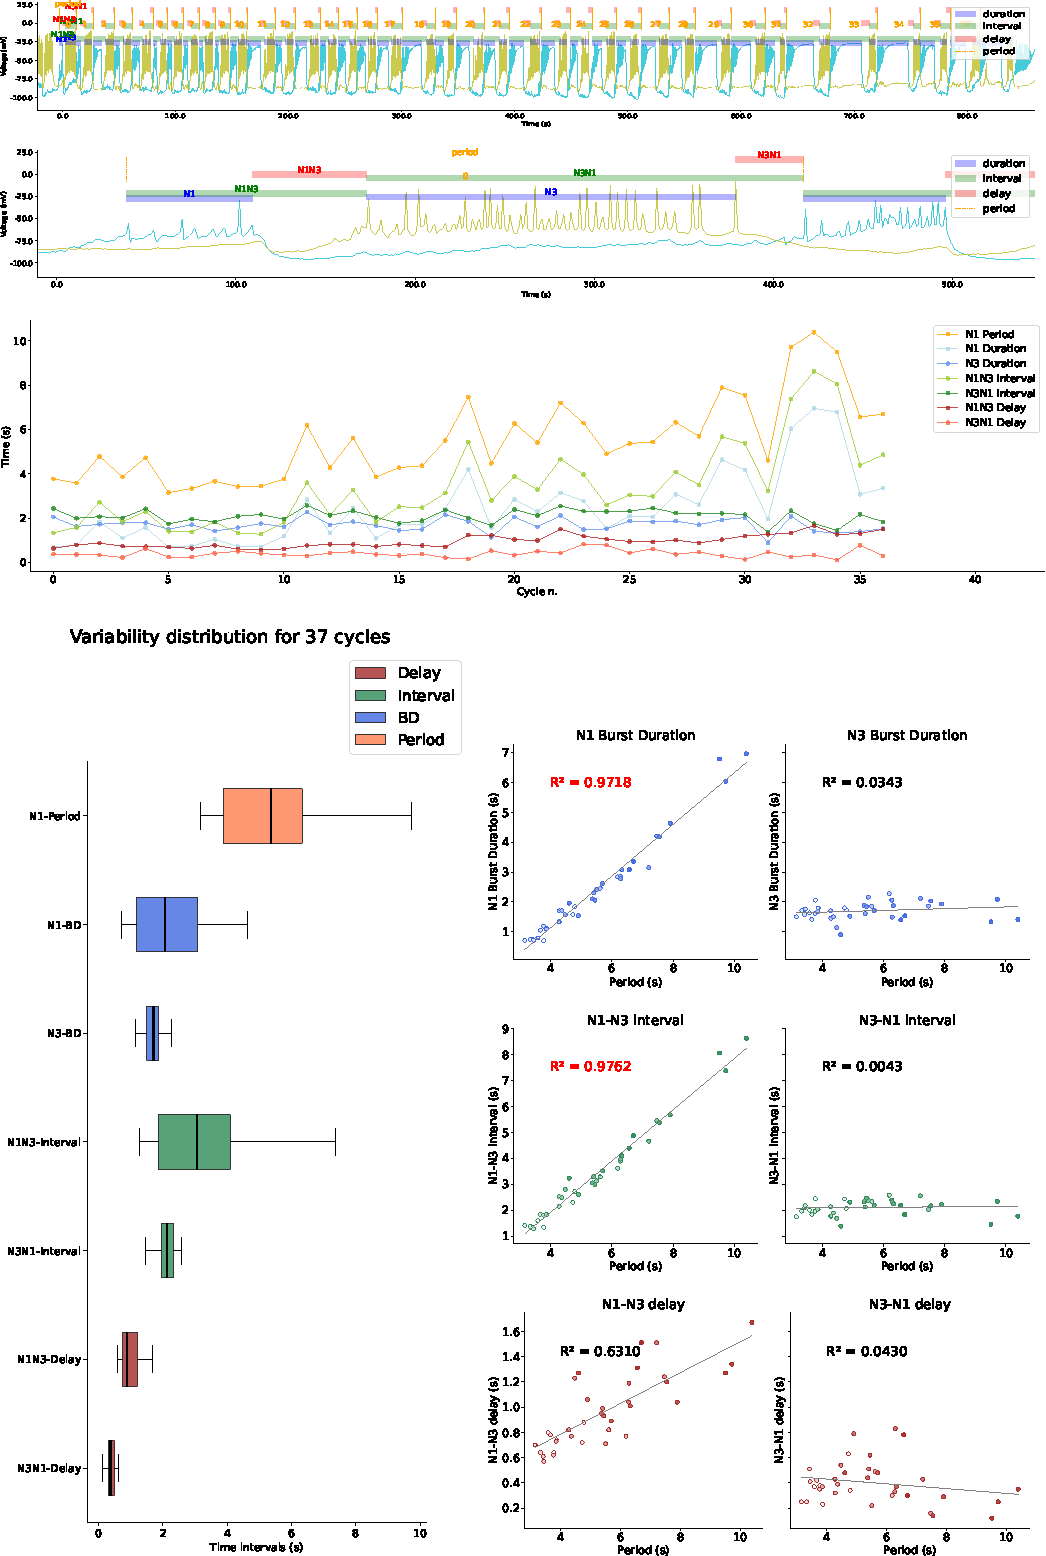
\includegraphics[width=0.9\textwidth]{./invariants/data/SUSSEX/MLN_driven/images/panel_with_intervals.pdf}
	\caption{\textbf{MLN stimulation}: Panel of intervals distribution and dynamical invariants for the three phases in the CPG under MLN Medium Lip Nerve (MLN) stimulation.}
	\label{fig:mln stimulation}
\end{figure}


\begin{figure}[htbp]
	\centering
	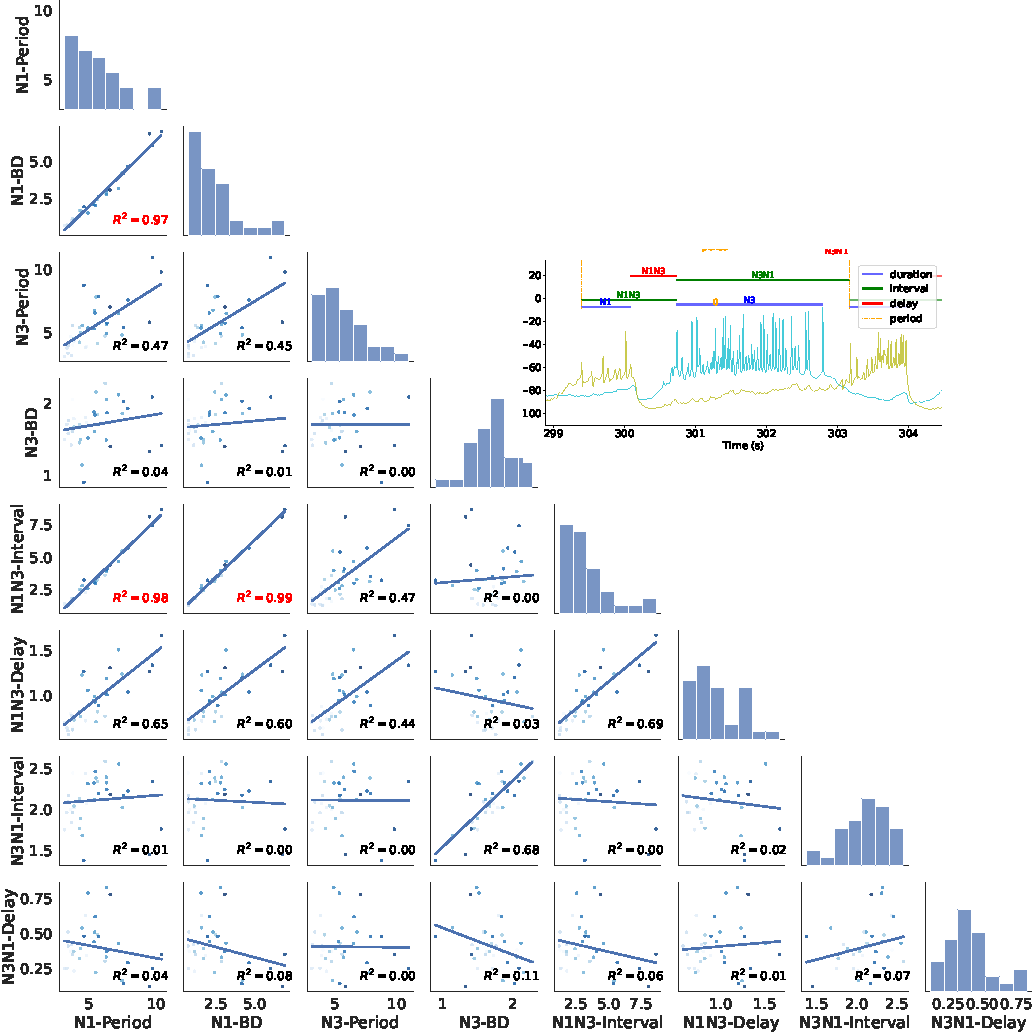
\includegraphics[width=0.9\textwidth]{./invariants/data/SUSSEX/MLN_driven/images/panel_with_pairplot.pdf}
	\caption{\textbf{MLN stimulation}:Pairplot of the invariants reset within cycles.}
	\label{fig:mln stimulation pairplot}
\end{figure}


\begin{figure}[htbp]
	\centering
	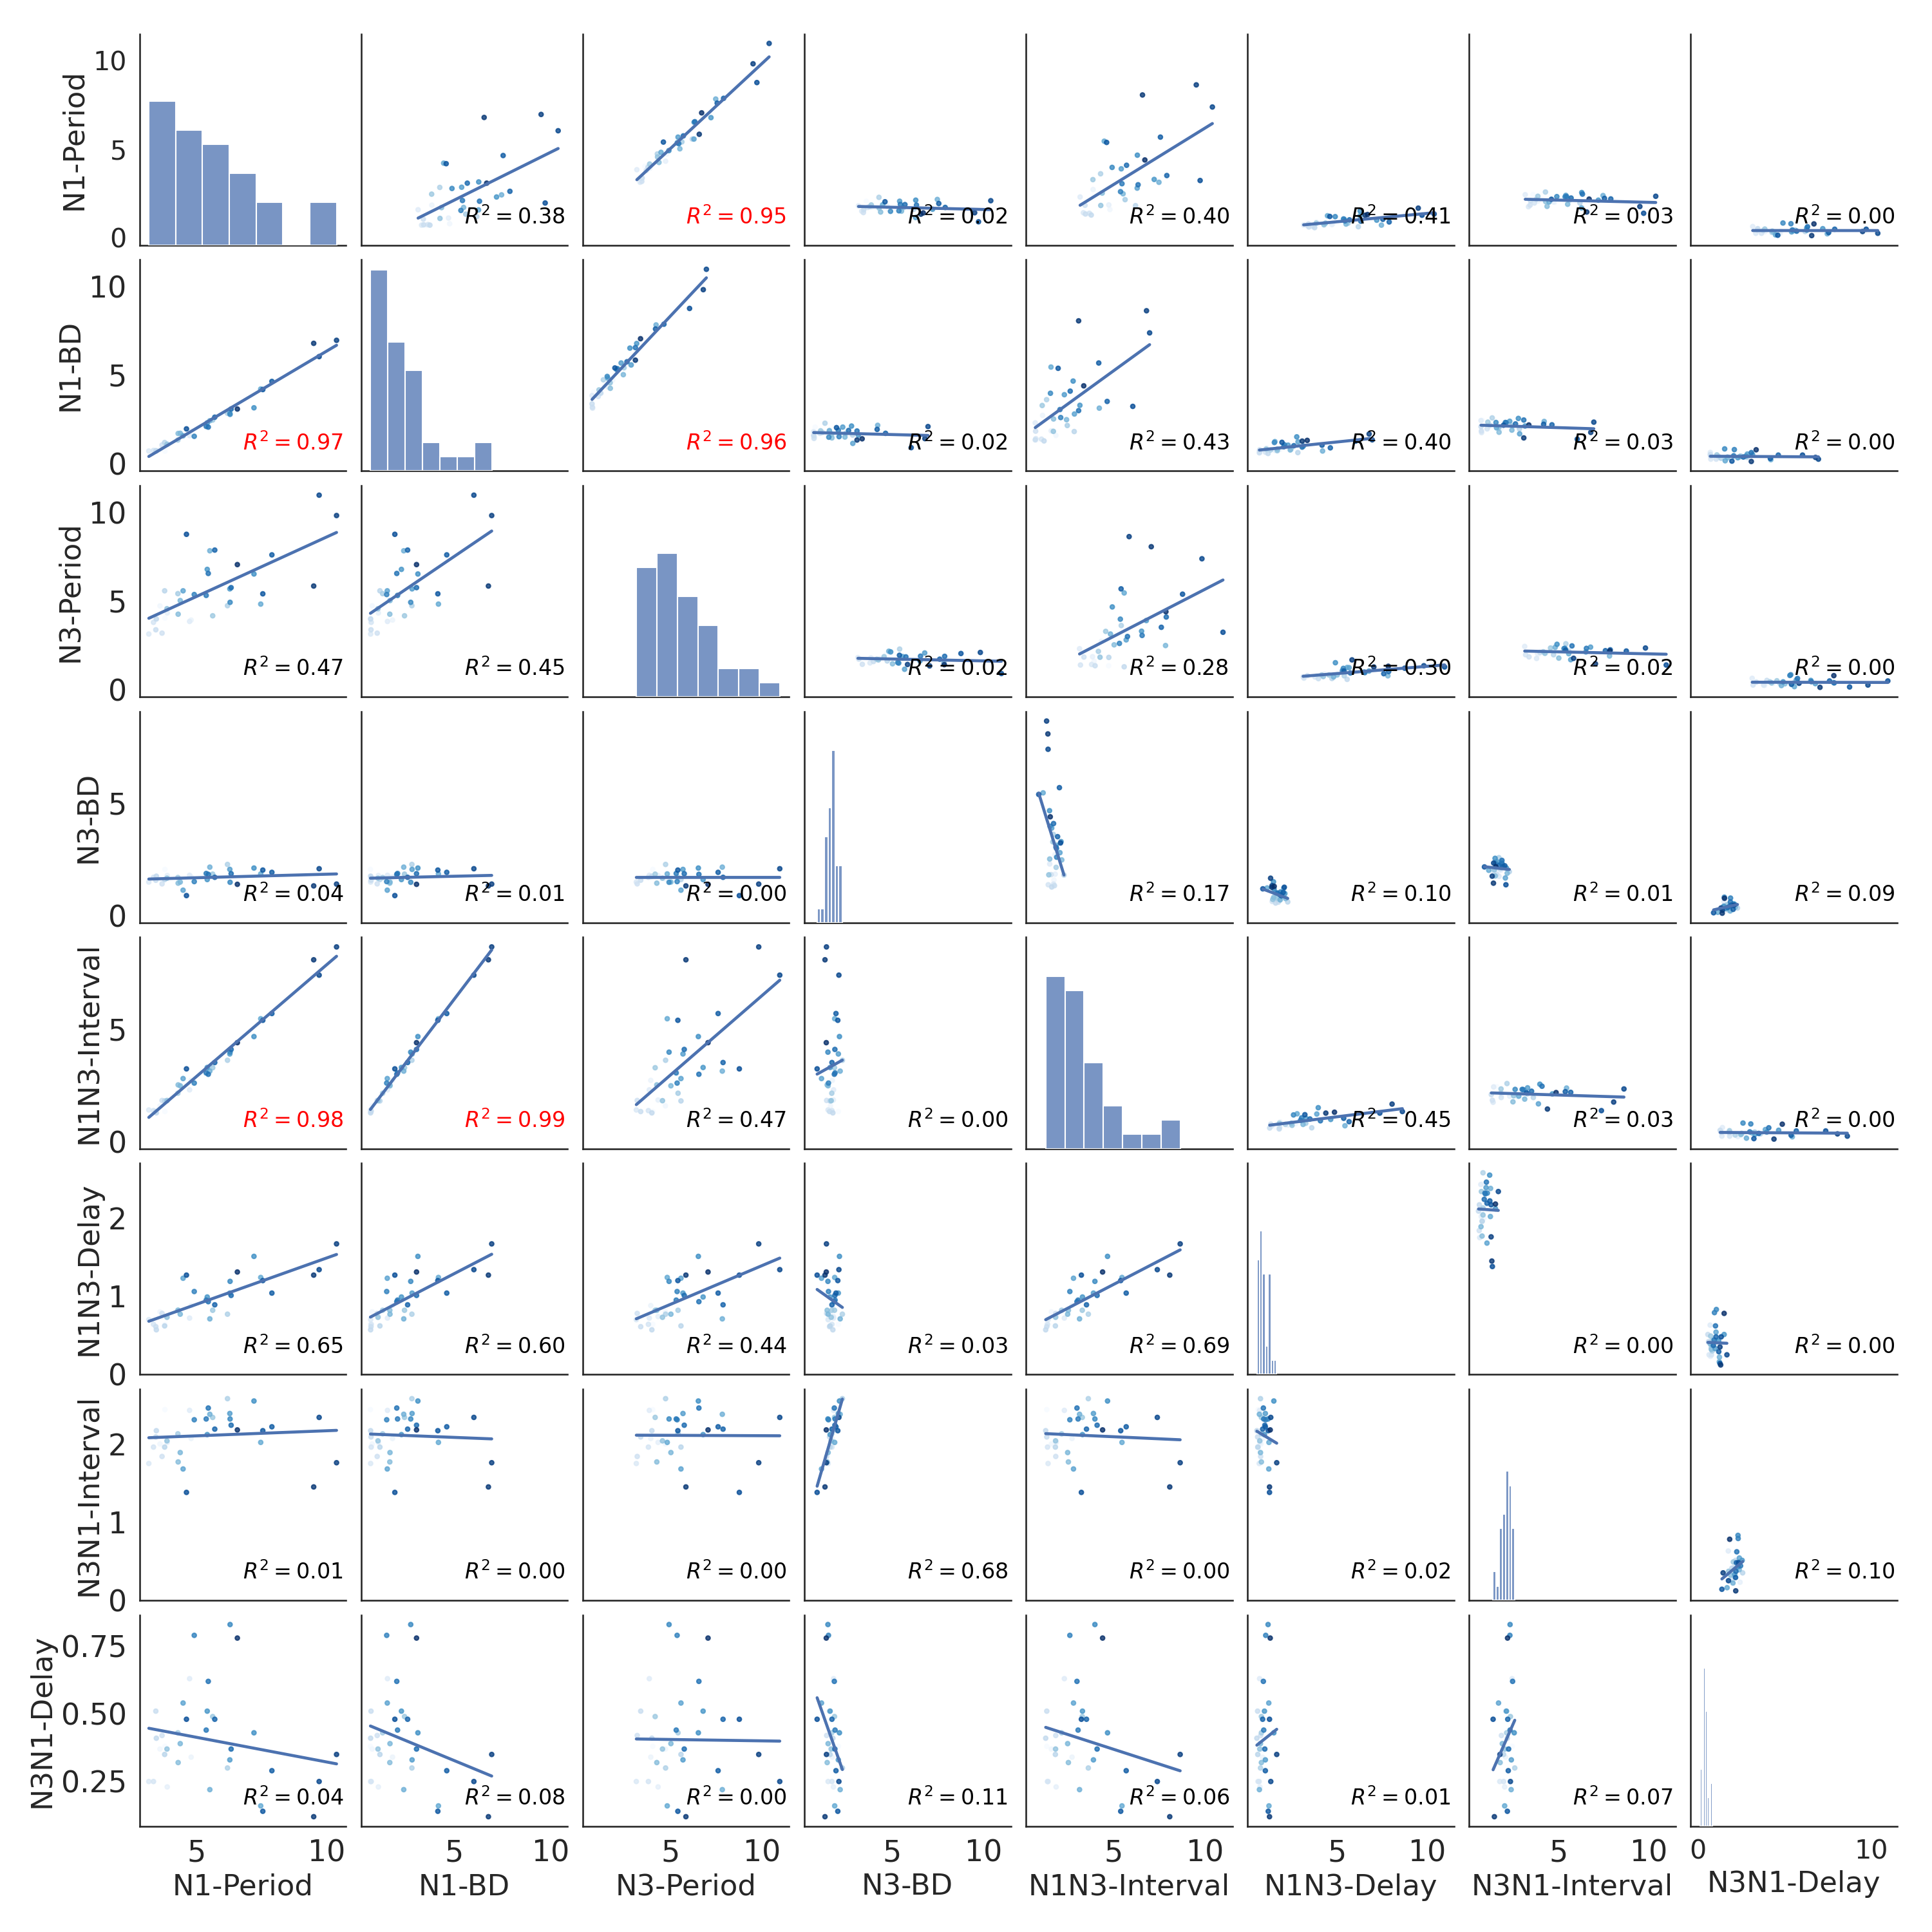
\includegraphics[width=0.9\textwidth]{./invariants/data/SUSSEX/MLN_driven/images/_output_pairplot_reset.png}
	\caption{\textbf{MLN stimulation}: Panel of intervals distribution and dynamical invariants for the three phases in the CPG under MLN Medium Lip Nerve (MLN) stimulation.}
	\label{fig:mln stimulation reset pairplot}
\end{figure}


\subsection{Invariants in cva1 stimulation driven activity}
CV1a is part of a larger population of CBIs 
%and the complete map of their locations is shown in Figure 3A. https://static-content.springer.com/esm/art%3A10.1186%2F2042-1001-2-4/MediaObjects/13232_2011_20_MOESM3_ESM.jpeg
Sucrose drives rhythmic activity in CBIs activating the feeding circuit by the conection
\paragraph{Example 1}

%\begin{figure}[htbp]
%	\centering
%	\includegraphics[width=0.9\textwidth]{./invariants/data/SUSSEX/CV1a_driven1/images/3phases/panel_with_intervals.pdf}
%	\caption{\textbf{CV1a driven case1}: Panel of intervals distribution and dynamical invariants for the three phases in the CPG under CV1a stimulation.}
%	\label{fig:cv1a 1 3phases}
%\end{figure}
%
%\begin{figure}[htbp]
%	\centering
%	\includegraphics[width=0.9\textwidth]{./invariants/data/SUSSEX/CV1a_driven1/images/3phases/panel_with_pairplot.pdf}
%	\caption{\textbf{CV1a driven case1}: Panel of intervals distribution and dynamical invariants for the three phases in the CPG under CV1a stimulation.}
%	\label{fig:cv1a 1 3phases pairplot}
%\end{figure}

\begin{figure}[htbp]
	\centering
	\includegraphics[width=0.9\textwidth]{./invariants/data/SUSSEX/CV1a_driven1/images/2phases/panel_with_intervals.pdf}
	\caption{\textbf{CV1a driven case1}:Panel of intervals distribution and dynamical invariants for the two phases in the CPG under CV1a stimulation.}
	\label{fig:cv1a 1 2phases}
\end{figure}


\begin{figure}[htbp]
	\centering
	\includegraphics[width=0.9\textwidth]{./invariants/data/SUSSEX/CV1a_driven1/images/2phases/panel_with_pairplot.pdf}
	\caption{\textbf{CV1a driven case1}:Panel of intervals distribution and dynamical invariants for the two phases in the CPG under CV1a stimulation.}
	\label{fig:cv1a 1 2phases pairplot}
\end{figure}



\paragraph{Example 2}


\begin{figure}[htbp]
	\centering
	\includegraphics[width=0.9\textwidth]{./invariants/data/SUSSEX/CV1a_driven2/images/panel_with_intervals.pdf}
	
	\caption{\textbf{CV1a driven case2}: Panel of intervals distribution and dynamical invariants for the two phases in the CPG under CV1a stimulation.}
	\label{fig:cv1a 2 2phases}
\end{figure}


\begin{figure}[htbp]
	\centering
	\includegraphics[width=0.9\textwidth]{./invariants/data/SUSSEX/CV1a_driven2/images/panel_with_pairplot.pdf}
	
	\caption{\textbf{CV1a driven case2}: Panel of intervals distribution and dynamical invariants for the two phases in the CPG under CV1a stimulation.}
	\label{fig:cv1a 2 2phases pairplot}
\end{figure}




\paragraph{Example 3}


\begin{figure}[htbp]
	\centering
	\includegraphics[width=0.9\textwidth]{./invariants/data/SUSSEX/CV1a_driven3/images/panel_with_intervals.pdf}
	\caption{\textbf{CV1a driven case3}: Panel of intervals distribution and dynamical invariants for the two phases in the CPG under CV1a stimulation.}
	\label{fig:cv1a 3 2phases}
\end{figure}



\paragraph{Example 4}

%\begin{figure}[htbp]
%	\centering
%	\includegraphics[width=0.9\textwidth]{./invariants/data/SUSSEX/CV1a_driven4/images/3phases/panel_with_intervals.pdf}
%	\caption{\textbf{CV1a driven case 4}: Panel of intervals distribution and dynamical invariants for the three phases in the CPG under CV1a stimulation.}
%	\label{fig:cv1a 4 3phases}
%\end{figure}
%
%\begin{figure}[htbp]
%	\centering
%	\includegraphics[width=0.9\textwidth]{./invariants/data/SUSSEX/CV1a_driven4/images/3phases/panel_with_pairplot.pdf}
%	\caption{\textbf{CV1a driven case 4}: Panel of intervals distribution and dynamical invariants for the three phases in the CPG under CV1a stimulation.}
%	\label{fig:cv1a 4 3phases pairplot}
%\end{figure}

\begin{figure}[htbp]
	\centering
	\includegraphics[width=0.9\textwidth]{./invariants/data/SUSSEX/CV1a_driven4/images/2phases/panel_with_intervals.pdf}
	\caption{\textbf{CV1a driven case4}: Panel of intervals distribution and dynamical invariants for the two phases in the CPG under CV1a stimulation.}
	\label{fig:cv1a 4 2phases}
\end{figure}

\begin{figure}[htbp]
	\centering
	\includegraphics[width=0.9\textwidth]{./invariants/data/SUSSEX/CV1a_driven4/images/2phases/panel_with_pairplot.pdf}
	\caption{\textbf{CV1a driven case4}: Panel of intervals distribution and dynamical invariants for the two phases in the CPG under CV1a stimulation.}
	\label{fig:cv1a 4 2phases pairplot}
\end{figure}

\subsection{Summary}
\begin{figure}
	\includegraphics[width=\textwidth]{./invariants/styled_table_invariants_r-squared.pdf}
	\caption{Table of $R^2$ values for the linear regression between the period and each interval for all experimental recordings showed in this section.}
	\label{fig:R2 table}
\end{figure}

\begin{figure}
	\includegraphics[width=\textwidth]{./invariants/styled_table_invariants_r-value.pdf}
	\caption{Table of $R$ values for the linear regression between the period and each interval for all experimental recordings showed in this section.}
	\label{fig:R table}
\end{figure}




\section{Characterization of variability in bursting models and its functionality}
\label{sec:model variability}
Bursting dynamics has been extensively studied in a wide variety of neural systems, as it is instrumental for many brain functions, including motor coordination and cognitive performance, and can be related to both healthy and pathological states. Neuronal models in computational neuroscience often reproduce key functional features of their biological counterparts. However, they also present limitations such as their poor ability to mimic the observed intrinsic variability of living neurons, particularly in membrane potential waveforms and in collective adaptive dynamics. Biophysical models typically produce stereotyped fixed membrane potential depolarization and repolarization waveforms, and restricted dynamical flexibility as compared to those observed in experimental recordings. Variability in the activity of living neurons has been proven to play an important role in relevant information processing tasks. We have seen in this chapter, the importance of variability in the presence of sequential dynamical invariants in the bursting activity and the limitations of studying them in a model when the variability is induced by a current ramp stimulation. The variability in models has usually been induced by gaussian noise, but this ignores the importance of the functional variability in the neurons, the observed variability is not only a cause of stochastic alterations but a functional outcome. 

In this section, we will describe this variability characteristics in experimental recordings, not only regarding the sequence time-intervals but also their waveforms. We will compare this variability with that of classical models and models able to produce chaotic activity. 
Figure \ref{fig:lp-pd burst variability} shows examples of the bursting and waveform variability in the intracellular recordings of LP and PD neurons in the pyloric CPG of \textit{Carcinus maenas}. In both neurons, we can appreciate a wide variability in the burst shape and duration, including the variability in the hyperpolarization.

\begin{figure}[hbt]
	\centering
	\begin{minipage}{0.48\textwidth}
		\includegraphics[width=\textwidth]{img/invariants/variability/lp_burst_variability.png}
	\end{minipage}
	\begin{minipage}{0.48\textwidth}
		\includegraphics[width=\textwidth]{img/invariants/variability/pd_burst_variability.png}
	\end{minipage}
	\caption{Example of variability in waveforms from intracellular recordings of the LP and PD neurons in the pyloric CPG}
	\label{fig:lp-pd burst variability}
\end{figure}

Although models can faithfully reproduce the activity and shape of neural models, they usually fail on reproducing the intrinsic and collective variability that we observe in electrophysiological recordings, this is the case for example of \textcite{hodgkin_quantitative_1952} or \textcite{vavoulis_dynamic_2007}, represented in Fig. \ref{fig:model burst no variability}. In that reproduction, although the waveform shape is accurate, the functional variability is hindered, reproducing a tonic and steady bursting activity. 

\begin{figure}[hbt]
	\centering
	\begin{minipage}{0.48\textwidth}
		\includegraphics[width=\textwidth]{img/invariants/variability/GHmodel.png}
	\end{minipage}
	\begin{minipage}{0.48\textwidth}
		\includegraphics[width=\textwidth]{img/invariants/variability/N1Mnovar.png}
	\end{minipage}
	\caption{Example of bursts with no variability in waveforms from model simulation of neuron from \textcite{ghigliazza_minimal_2004b} model in chaotic mode and N1M neuron from \textcite{vavoulis_dynamic_2007} with no ramp stimulation in the CPG circuit. The equations for both models can be found in Secs. \ref{sec:model variability equations} and \ref{sec:CPG model equations}, respectively.}
	\label{fig:model burst no variability}
\end{figure}



In section \ref{sec:CPG model equations}, we saw that variability can be induced by including a current ramp, although it can reproduce the variability, when studying the activity cycle-by-cycle it hinders the functional variability of the spontaneous activity. 


\begin{figure}[hbt]
	\centering
	\begin{minipage}{0.48\textwidth}
		\includegraphics[width=\textwidth]{img/invariants/variability/TN-burst_variability.png}
	\end{minipage}
	\begin{minipage}{0.48\textwidth}
		\includegraphics[width=\textwidth]{img/invariants/variability/n1m_vav_burst_variability.png}
	\end{minipage}
	\caption{Example of variability in waveforms from model simulation of neuron from \textcite{nowotny_probing_2008} model in chaotic mode and N1M neuron from \textcite{vavoulis_dynamic_2007} under current stimulation in the CPG circuit. The equations for both models can be found in Secs. \ref{sec:model variability equations} and \ref{sec:CPG model equations}, respectively.}
	\label{fig:model burst variability}
\end{figure}


Modern experimental techniques involving activity-dependent electrical, optical and chemical stimulation can further unveil and explain functional variability of bursting sequences in a wide variety of nervous systems, it is important to rely on models able to reproduce the intrinsic variability. It will also be relevant for designing associated applications in the context of neurotechnology, artificial intelligence and robotics \parencite{garrido-pena_exploring_2024}. 

%
%In this work, we illustrate that current biophysical neuron models fail to reproduce the intrinsic and collective variability observed in electrophysiological recordings in the nervous system of different animals, and how this hinders the theoretical study of the relevance of sequential neural dynamics. We also assess the solution to this problem in well-known bursting neuron models by identifying possible biophysical and synaptic candidates that can explain the observed variability while sustaining the robustness of the model oscillatory activity. Finally, we discuss the importance of model intrinsic variability in the context of biohybrid circuits built with interacting living and model neurons to evaluate the role of robust sequential neuronal and circuit dynamics in motor function coordination.

%Bursting dynamics has been extensively studied in a wide variety of neural systems, as it is instrumental for many brain functions, including motor coordination and cognitive performance, and can be related to both healthy and pathological states. Much less attention has been paid to the emerging sequential dynamics that underlies many rhythms built with bursting dynamics. Neural bursting activity provides robust temporal references to define time intervals that build sequences that repeat themselves, frequently at different time scales. The study of the variability of sequence time intervals is relevant to understand the balance between robustness of the order of the neural sequence and the flexibility in timing and duration required for the coordination of specific neural functions. The characterization of time intervals underlying bursting sequences has recently yielded the discovery of sequential dynamical invariants in the form of robust cycle-by-cycle relationships among specific intervals that coexist with other intervals whose variability remains unrelated. Sequential dynamical invariants have been proposed to underlie the dynamical coordination in motor circuits that produce rhythmic movements.  

%In this work we expose, reproduce and explain the variability observed in sequential neural bursting dynamics using a combination of experiments, sequence interval data characterization tools and computational models. Our experimental analysis shows that sequential dynamical invariants only exist if sufficient variability is present, and they can be linked to asymmetrical circuit topologies and multiple synaptic timescales. Traditional bursting neural models lack the observed experimental variability but can nevertheless display sequential dynamical invariants from external perturbations or an adequate combination of intrinsic neuron and synaptic dynamics. Modern experimental techniques involving activity-dependent electrical, optical and chemical stimulation can further unveil and explain functional variability of bursting sequences in a wide variety of nervous systems, and to design associated applications in the context of neurotechnology, artificial intelligence and robotics.  
%
%Additional information 
%
%We characterized the activity of bursting neural sequences in two distinct Central Pattern Generator (CPG) circuits (Lymnaea Stagnalis and Carcinus maenas) using long intracellular and extracellular electrophysiological recordings and in their corresponding conductance-based models. We addressed both intrinsic and extrinsic variability with control recordings and perturbations induced by electrical, chemical, optical and biohybrid circuits composed of living and model neurons. We found that robust sequences coexisted with a wide variability in cycle-by-cycle periods and intervals constituting the sequence (see panel A in Fig. 1). We characterized the variability in waveform (panels B-D) and time intervals defined from the beginning and the end of the bursting activity (panels E-F). Specific cycle-by-cycle sequence intervals displayed strong linear (marked with purple asterisks in panels E-F) or nonlinear relations indicating dynamical constraints to the sequential coordination while others had unrelated variability allowing flexibility in timing and duration. Our model analysis showed that invariants emerged when the synaptic mechanisms allow the propagation of the variability through nonsymmetrical mechanisms and rich transient neuronal dynamics. We have developed protocols and analysis tools that have a general use to expose and characterize dynamical invariants in a wide variety of nervous systems, which will serve to validate the universality of this phenomenon and to link it to functionality and healthy and pathological states, including novel neurotechnology design. 




\section{Transformation of sequential intervals into effective robot movement}
\label{sec:robot}
To validate the importance of the balance between robustness and flexibility in  CPG circuits, as provided by the cycle-by-cycle dynamical invariants present in the dynamics discussed in this chapter, we include in this section a validation experiment for the translation of dynamical invariants into an effective motor locomotion in a Functional-Living-Circuit-Hybrot (FLC-Hybrot) \parencite{amaducci_hybrid_2020,amaducci_controlling_2021,soetard_dynamical_2023}. The combination of models, novel tools and experimental approaches has proven its effectiveness in revealing and exploring features of neural dynamics \parencite{szucs_interacting_2000,chamorro_generalization_2012,reyes-sanchez_automatized_2023}. In this first step into the applications in robotics of the variability time constrains found in CPGs, we built an hexapod robot whose legs performed oscillatory activity to move forward. The period and amplitude of these oscillations were determined by the sequential cycle-by-cycle activity of the CPG neurons recorded from the living preparation and sent online to the robot. At the same time, the hybrot included a light sensor and sent feedback information regarding the light conditions around it back to the neural circuit in the form of an electrical current. These stimuli modified the behavior of the cells, resulting in a change of the hybrot locomotion, preserving always the required motor coordination, and therefore forming a real-time closed-loop interaction among living and electronic components (Figure \ref{fig:robot_results_summary} shows a summary of these interactions). The goal of the FLC-Hybrot is to demonstrate that a dynamical principle of the functional living circuit can be used to autonomously coordinate the locomotion with sensory feedback from the robot. In our case, we used the presence of dynamical invariants in the form of robust relationships between the time intervals that build the cycle-by-cycle activity of the neurons of the pyloric CPG in \textit{Carcinus maenas}, which are sustained under any circumstance, even when there are external inputs to the circuit, to modulate the behavior of the robot. Section \ref{sec:robot setup} provided a detailed description of the experimental setup for the hybrot. 

\begin{figure}[hbt!]
	\begin{center}
		% \includegraphics[width=\linewidth]{images/robot/robot_results_summary}
		\includegraphics[width=\textwidth]{img/invariants/robot/Figure1_experiment_design_v1.png}
	\end{center}
	\caption{Representation of the FLC-Hybrot paradigm design. Neural dynamics from a functional living CPG circuit are recorded online and used to coordinate the robot movement in real-time. Activity from the PD neuron is recorded intracellularly (green trace), while the LP bursts are extracted from the nerve's extracellular signal (blue trace). This robot walks through a trial track with interspersed light and shadow regions. When the robot's light sensor detects that it is located under a shadow, it sends feedback current to the living circuit. CPG dynamics change as a reaction to the injected current, thus modifying the robotic locomotion. The following video shows an example of this experiment \url{https://youtu.be/ny2dJGbG8lo}.}
	\label{fig:robot_results_summary}
\end{figure}


To validate the adequate locomotion of the FLC-Hybrot when driven by the pyloric CPG online behavior, as well as the living circuit real-time adaptation to the injected feedback, we performed a set of experiments employing a 1.5 meters long trial track. Along this surface there were interspersed segments of lights and shadows. This configuration caused the FLC-Hybrot to alter its behavior several times during the experiment due to the injection of current into the PD neuron when it walked under a shadow. The current injected in the cell in a shadow section varied from one experiment to another, according to the neurons response to the stimuli. No current was injected when the robot was located on a luminous area. The following video illustrates one of such experiments \url{https://youtu.be/Dltec7TeGso}.

\begin{figure}[hbt!]
	\begin{center}
		\includegraphics[width=0.8\linewidth]{./img/invariants/robot/robot_results_validation}
	\end{center}
	\caption{Flexible hybrot adaptation to environmental changes when noticed by the robot sensors and associated coordinated locomotion. When the robot entered a shadow section, it sent sensory feedback to the living CPG in the form of positive electrical current (red trace). Blue and green traces are recordings of the extracellular and intracellular (PD neuron) activity of the circuit and display the change caused by the feedback current injection in the PD neuron, slowing down the CPG rhythm. The oscillatory movement of the robot legs is represented in the brown trace and it can observed that a variation in the CPG rhythm leads to a change in the robotic locomotion, modifying both the period and the amplitude of the oscillation. 
		%This effect can be seen more clearly in the bottom panel, where both the LP neuron instantaneous bursting period (blue) and the robot legs oscillation period (brown) are plotted together, showing how the latter is modulated by the former.
	}
	\label{fig:robot_results_validation}
\end{figure}

Figure \ref{fig:robot_results_validation} shows the results for one of these tests. We observe a change in the neural activity when -0.6nA current is inserted into the PD neuron, causing the CPG rhythm to slow down while also modifying the PD neuron membrane's potential amplitude. This change is immediately reversed as soon as the current goes back to zero, restoring its previous behavior. Concerning the robot's locomotion, a variation in the legs' oscillation is observed just after the neurons alter their activity. Despite the successive changes in the amplitude and period of its legs' oscillation, the FLC-Hybrot maintained a coordinated and effective locomotion during the whole experiment. 

We know that in the pyloric CPG there is a sequential dynamical invariant, in the form of a linear relation between the LP neuron period and the LPPD interval. These are the intervals used to modulate the amplitude and period of the legs oscilation in the robot. This constrain was effectively transferred to the robot locomotion. Figure \ref{fig:robot_results_invariant} shows a comparison between the living CPG and the robot dynamical invariant, with the later reaching an $R^2$ correlation of 0.87 despite the lack of precision of its servomotors. It displayed the same correlation between its legs oscillation period and amplitude, which were modulated by the two previous temporal intervals. The methodological details for the legs tracking to characterize the effective transfer of the invariants can be found in \textcite{swarc_realtime_2023}.

\begin{figure}[hbt!]
	\begin{center}
		\includegraphics[width=\linewidth]{./img/invariants/robot/robot_results_invariant}
	\end{center}
	\caption{\textbf{Left:} dynamical invariant present in the living CPG activity during the validation test, represented as a cycle-by-cycle linear relation between the LP neuron bursting period and the LPPD interval. \textbf{Right:} dynamical invariant present in the FLC-Hybrot locomotion during the validation test, represented as a cycle-by-cycle linear relation between its legs' oscillation period and amplitude. The dynamical invariant property is effectively translated from the living CPG to the robot locomotion, encoded as: Robot period = LP period, Robot amplitude = LPPD interval * factor.}
	\label{fig:robot_results_invariant}
\end{figure}

This hybrot scenario can help simulate context change situations in which the CPG rhythm is modulated by external factors and there is a change of variability reflected in the relations between the cycle-by-cycle intervals. The reproduction of biological dynamics with preserved coordination time constraints can have strong implications in autonomous robot locomotion, and also in neurorehabilitation technologies. Under the scope of sequential dynamical invariants,  coordination rules are not imposed as conditional commands but autonomously emerge from the intrinsic sequential dynamics.

\section{Discussion}
In this chapter, we studied the sequentially analyzing the bursting activity of the feeding CPG in \textit{L. stagnalis}. As discussed before, this CPG is ideal for this kind of study due to their ability to maintain a robust sequential activation and still present a high flexibility to adapt to changes in the context. Also, the bursting activity provides clearer references than in other more complex circuits. 

In this system addressed the characterization of the intervals building up the rhythmic sequence in this system with model simulations and also in experimental intracellular recordings. We tested the presence of sequential dynamical invariants in the form of linear relationships between the sequence intervals and the cycle period of the rhythm following the experimental results that we reported in \textcite{elices_robust_2019} for the crustacean pyloric CPG. Most extended studies usually study the averaged variability, masking the information in the relations taking place at each cycle of sequential activations. Taking that into account, here we characterize the variability cycle-by-cycle. 

In the model, we extended the analysis of the reported relations by \textcite{Elliott1991} by characterizing each and every interval building the sequence and relating the strong linear relationships found in specific intervals to the concept of robust sequential dynamical invariants proposed in \textcite{elices_robust_2019} for the coordination of robust yet flexible CPG rhythms. In the simulations, three main cases have been addressed in the analysis: N1M-driven, SO-driven and N3t-driven stimulation. This was based on the two different possibilities of inducing variability in the model according to the results reported in \textcite{vavoulis_dynamic_2007}, as well as with a third neuron stimulation (N3t) which is easily addressable in the model circuit. When variability arises by the stimulation of N1M, the results are rather similar to the ones obtained stimulating N3t. Strong linear correlations to the period, i.e.,  dynamical invariants, are present mainly in all intervals related to N3 phase, since these are the ones with cycle-by-cycle variability related to the period variability.  

We also show the redistribution of variability that takes place when the stimulation is applied on SO. In this scenario more intervals presenting large variability than in the other stimulation protocols are found. This is due to the specific variability of N1M and N3t burst duration, since in this case the largest influence on the period seems to come not only from N3t but also from N1M. Hence, consequently to the variability analysis, different linear relationships are found involving all intervals related to N3 and N1 phases. The intervals unrelated to the period are the ones associated with N2 phase, which is also the least variable entity in the circuit. 

These results reproduce and extend the ones discussed in \textcite{vavoulis_dynamic_2007} and \textcite{Elliott1991}. It is interesting to highlight the differences in the results when the period is driven by N1M/N3t or SO. When the variability is induced in N1M/N3t, N3t is still able to inhibit the N1M neuron carrying the main variability, while SO is adapting to both. However, when SO is the neuron being stimulated, since it is connected to N1M by mutual excitation, they are both boosting each other's activity, leading to the higher variability of N1M. Here, N3t must adapt to N1M, which is harder due to the SO constant excitation. For this reason, it was necessary to inject some additional current in N3t in the simulations, which would usually be an input received from the cerebral ganglia. 

Each of the three phases of the rhythm corresponds to a specific motor action: N1 protraction, N2 rasp and N3 swallow. As it is pointed out in \textcite{Elliott1991}, the motor sequence consists of a two-stroke relaxation: protraction and rasp (N1,N2), in charge of moving the radula, and swallowing (N3). In these kind of systems, it is common to find one of them fixed and the other one variable, which in our case is the swallow phase. In this context, SO stimulation can be related to sucrose stimulation \textcite{benjamin_distributed_2012,kemenes_analysis_1994},
this could be related with the increase in N1M variability, since in presence of food, protraction phase may become crucial for an effective food reaching. Thus, there might be now two phases showing more variability in their intervals duration. The discussed invariants can participate in the coordination of these mechanisms by imposing  variability constraints in only specific intervals of the motor sequence. The results shown in this paper also indicate that distinct constraints in the form of dynamical invariants can emerge in the same network under different behavioral contexts.

The flexibility of this model to adapt the induced variability into the system is not an easy feature to achieve. Some characteristics in the description of this model such as the gradual synapse and the separation between fast and slow dynamics for each neuron, might be key achieving this. Although this realistic definition of the interrelations between the neurons in the CPG in this model, allowed the study of dynamical invariants, inducing the variability by a current ramp injection hinders the functional variability generated by the neurons and the spontaneous activity of the neurons. We saw this limitation when study the experimental intracellular recordings, where spontaneous activity and induced modulation recordings, showed the variability cycle-by-cycle, and the stochastic sequence of time-interval durations. 

In the experimental study, even under those scenarios of high stochasticity, we showed that there were strong linear relationships in the form of sequential robust dynamical invariants in some of the intervals. Also, as we observed in the model, depending on the source of the activation, the distribution of variability and the intervals presenting this strong relationships changed. In the case of spontaneous activity, we found a different situation for each, the most robust example was a strong linear correlation for N3 phase, in a recording where the N3 seemed to be inducing periods of silence. In the other two cases, the variability was shifted, having N1 a larger relation to the period cycle-by-cycle and with a distribution of variability between both. What we saw in this case, and in the rest of the experiments in that section, was the absence of relation between N2 phase and the period, which means, the variability in each cycle is not carried by the rasp phase, which has a constant and low variable activation. Apart from the spontaneous recording, we analyzed three cases of CPG activity modulation: SO neuron driven, MLN stimulation and CV1a neuron driven. Each case is associated to a different source or modulation of the activity, with functional processes related and for each one we observed a different distribution of the variability between the time-intervals. During the SO modulation, in spontaneous and induced scenarios we saw, as in the model, that variability was carried by N1 and N3 phases, having both relation to the period cycle-by-cycle, being stronger in the case of N1. When stimulating the middle lip nerve (MLP), directly connected to the N1M to activate the rhythm, there was a robust sequential dynamical invariant in N1, showing that during this activation (in the simulated presence of food) the role of protraction phase was key, carrying all variability. Finally in the CV1a neuron stimulation, the N1 phase was again the one with a larger relation to the period, showing also that a small change in that stimulation, altered the distribution of variability shifting to N3 phase and the related intervals. 

With these results, we saw the potential of dynamical invariants as functional variability indicators, since they reflect a balance between the robustness of the sequence and the flexibility to accommodate longer or shorter intervals from the network interaction. The distinct sources of feeding activation changed the classification of variability, adjusting the importance from one phase to another. Also, in the model we saw that this phenomena is highly dependent on the intrinsic dynamics, network topology and synaptic dynamics that contribute to the generation of the dynamical invariants. Their observation in the model simulations where only possible when other neurons in the circuit adapted their activity to the neuron with the induced variability. 

The study of cycle-by-cycle invariant relationships, found not only in experimental recordings but also in computational models as we report here, highlights the presence of organized variability in a motor rhythm. This points to the universality of this phenomena, and the functional associations to it show its potential as time indicator. The applications to this indicator can be key for future clinical applications, specially for novel neurotechnology tools. In this line, we showed a first approach of the extrapolation of this restrictions into an effective locomotion in the FLC-Hybrot. The hexapod robot  showed that it is possible to translate the dynamical invariants into the relation between the oscillation amplitude and period, showing the possible future applications of locomotion based on the CPG features. This study paves the way for further exploration of dynamical invariants in more complex neural systems and their practical applications.




% It is important to emphasize that in this CPG model the variability was induced by applying a current ramp to N1M, N3t or SO neurons. Sources of intrinsic variability in circuit models can include the use of chaotic neurons \textcite{elices_closed-loop_2015,elices_asymmetry_2017} or noise. We However, in our experience so far, such variability is not enough to generate dynamical invariants while sustaining robust rhythms in the circuit. On the other hand, living neurons variability can be propagated to model neurons to generate dynamical invariants in hybrid circuit configurations of interacting artificial and living neurons \textcite{amaducci_rthybrid_2019,reyes-sanchez_automatic_2020}.

% Invariants reflect a balance between the robustness of the sequence and the flexibility to accommodate longer or shorter intervals from the network interaction. The isolated and network behavior of the feeding CPG neurons was studied in~\textcite{straub_endogenous_2002}, which showed the capacity of isolated N1M neurons to generate a plateau. When neurons are connected, features such as the N2v characteristic waveform or the N3t post inhibitory rebound emerge. Our model study indicates that intrinsic dynamics, network topology and synaptic dynamics contribute to the generation of the dynamical invariants.



% Previous results that indicated the existence of these invariants in \textit{Lymnaea Stagnalis} when stimulating two specific neurons have been reproduced computationally using Vavoulis et al. CPG feeding model and providing a wider analysis of variability, not only in the burst duration intervals but in a complete set of intervals obtained from the relation between different neurons.

% The presence of dynamical invariants in another CPG beyond the already found in \textit{Carcinus maenas} \textcite{elices_robust_2019} points out to a general phenomena that can be present in other more complex sequence generating neural systems. Moreover, the results reported in this paper indicate that such invariants can be found in computational models with sufficiently rich intrinsic and circuit dynamics.







% Hybrots constitute an useful resource to study neural circuits dynamics and their relationship to behavior since they provide an artificial powerplant to implement experiments that otherwise would lack one, like those performed \textit{in vitro} or \textit{in vivo} with immobilized animals. In our particular case, we designed FLC-Hybrot to analyze how the dynamical invariants present in the \textit{Carcinus maenas} pyloric CPG could be applied for the coordination of robotic locomotion. We validated that when modulated by these temporal intervals, the oscillatory motion of the robot legs remained coordinated at all times, despite all the variations in amplitude and period that took place during the experiments. Moreover, video tracking of the hybrot movement revealed that dynamical invariants were effectively translated into the relation between the oscillation amplitude and period. This resulted in a more stable and constant movement speed for the hybrot than when coordinated by intervals that did not maintain a dynamical invariant relationship.

